% Created 2021-05-24 Mon 19:27
% Intended LaTeX compiler: pdflatex
\documentclass{tufte-book}
\usepackage[utf8]{inputenc}
\usepackage[T1]{fontenc}
\usepackage{graphicx}
\usepackage{grffile}
\usepackage{longtable}
\usepackage{wrapfig}
\usepackage{rotating}
\usepackage[normalem]{ulem}
\usepackage{amsmath}
\usepackage{textcomp}
\usepackage{amssymb}
\usepackage{capt-of}
\usepackage{hyperref}
\hypersetup{colorlinks}% uncomment this line if you prefer colored hyperlinks (e.g., for onscreen viewing)
\usepackage{amsfonts, soul, microtype}



%toc
%\usepackage{titletoc}
%

% section and subsection headings
\usepackage{titlesec}

\titleformat{\section}
  {\normalfont\fontsize{12}{15}\bfseries}{\thesection}{1em}{}

\usepackage[linesnumbered, ruled]{algorithm2e}
\usepackage{algorithmic}
\usepackage[parfill]{parskip}

%\usepackage{thmtools}
%\theoremstyle{definition}
\newtheorem{theorem}{Theorem}[chapter]
\newtheorem{lemma}[theorem]{Lemma}
\newtheorem{corollary}[theorem]{Corollary}
\newtheorem{proposition}[theorem]{Proposition}
\newtheorem{property}[theorem]{Property}
\newtheorem{fact}[theorem]{Fact}
\newtheorem{problem}[theorem]{Problem}
\newtheorem{exercise}[theorem]{Exercise}
\newtheorem{example}[theorem]{Example}
\newtheorem{definition}[theorem]{Definition}
\newtheorem{remark}[theorem]{Remark}
\newtheorem{conjecture}[theorem]{Conjecture}
\newtheorem{claim}[theorem]{Claim}

%Book metadata
%\title{A Tufte-Style Book\thanks{Thanks to Edward R.~Tufte for his inspiration.}}
%\author[The Tufte-LaTeX Developers]{The Tufte-LaTeX\ Developers}
%\publisher{Publisher of This Book}

%%
% If they're installed, use Bergamo and Chantilly from www.fontsite.com.
% They're clones of Bembo and Gill Sans, respectively.
%\IfFileExists{bergamo.sty}{\usepackage[osf]{bergamo}}{}% Bembo
%\IfFileExists{chantill.sty}{\usepackage{chantill}}{}% Gill Sans

%\usepackage{microtype}
\usepackage{hyperref}
%%
% Just some sample text

%%
% For nicely typeset tabular material
\usepackage{booktabs}

%%
% For graphics / images
\usepackage{graphicx}
\setkeys{Gin}{width=\linewidth,totalheight=\textheight,keepaspectratio}
\graphicspath{{graphics/}}

% The fancyvrb package lets us customize the formatting of verbatim
% environments.  We use a slightly smaller font.
\usepackage{fancyvrb}
\fvset{fontsize=\normalsize}

%%
% Prints argument within hanging parentheses (i.e., parentheses that take
% up no horizontal space).  Useful in tabular environments.
%\newcommand{\hangp}[1]{\makebox[0pt][r]{(}#1\makebox[0pt][l]{)}}

%%
% Prints an asterisk that takes up no horizontal space.
% Useful in tabular environments.
%\newcommand{\hangstar}{\makebox[0pt][l]{*}}

%%
% Prints a trailing space in a smart way.
\usepackage{xspace}


% Prints the month name (e.g., January) and the year (e.g., 2008)
\newcommand{\monthyear}{%
  \ifcase\month\or January\or February\or March\or April\or May\or June\or
  July\or August\or September\or October\or November\or
  December\fi\space\number\year
}


% Prints an epigraph and speaker in sans serif, all-caps type.
\newcommand{\openepigraph}[2]{%
  %\sffamily\fontsize{14}{16}\selectfont
  \begin{fullwidth}
  \sffamily\large
  \begin{doublespace}
  \noindent\allcaps{#1} \\ % epigraph
  \noindent\allcaps{#2}% author
  \end{doublespace}
  \end{fullwidth}
}
% Generates the index
\usepackage{makeidx}
\makeindex


\makeatletter
\renewcommand{\maketitlepage}{%
\begingroup%
\setlength{\parindent}{0pt}}

{\fontsize{24}{24}\selectfont\textit{\@author}\par}

\vspace{1.75in}{\fontsize{36}{54}\selectfont\@title\par}

\vspace{0.5in}{\fontsize{14}{14}\selectfont\textsf{\smallcaps{\@date}}\par}

\vfill{\fontsize{14}{14}\selectfont\textit{\@publisher}\par}

\thispagestyle{empty}
\endgroup

\makeatother

\titlecontents{part}%
    [0pt]% distance from left margin
    {\addvspace{0.25\baselineskip}}% above (global formatting of entry)
    {\allcaps{Part~\thecontentslabel}\allcaps}% before w/ label (label = ``Part I'')
    {\allcaps{Part~\thecontentslabel}\allcaps}% before w/o label
    {}% filler and page (leaders and page num)
    [\vspace*{0.5\baselineskip}]% after

\titlecontents{chapter}%
    [4em]% distance from left margin
    {}% above (global formatting of entry)
    {\contentslabel{2em}\textit}% before w/ label (label = ``Chapter 1'')
    {\hspace{0em}\textit}% before w/o label
    {\qquad\thecontentspage}% filler and page (leaders and page num)
    [\vspace*{0.5\baselineskip}]% after
%%%% End additional code by Kevin Godby
\author{nazaal}
\date{\today}
\title{}
\hypersetup{
 pdfauthor={nazaal},
 pdftitle={},
 pdfkeywords={},
 pdfsubject={},
 pdfcreator={Emacs 26.3 (Org mode 9.4.4)}, 
 pdflang={English}}
\begin{document}

\setlength\parindent{0pt}
\setcounter{secnumdepth}{2}
\newcommand{\indep}{\perp \!\!\! \perp}

\let\cleardoublepage\clearpage

\(\chapter*{Abstract}\)
Despite having a philosophical grounding from empiricism that spans some centuries, the algorithmization of causal discovery started only a few decades ago. This formalization of studying causal relationships relies on connections between graphs and probability distributions. In this setting, the task of causal discovery is to recover the graph that best describes the causal structure based on the available data. A particular class of causal discovery algorithms, called constraint-based methods rely on Directed Acyclic Graphs (DAGs) as an encoding of Conditional Independence (CI) relations that carry some level of causal information. However, a CI relation such as \(X\) and \(Y\) being independent conditioned on \(Z\) assumes the independence holds for all possible values \(Z\) can take, which can tend to be unrealistic in practice where causal relations are often context-specific.  In this thesis we aim to develop constraint-based algorithms to learn causal structure from Context-Specific Independence (CSI) relations within the discrete setting, where the independence relations are of the form \(X\) and \(Y\) being independent given \(Z\) and \(C=a\) for some \(a\). This is done by using Context-Specific trees, or CStrees for short, which can encode CSI relations. 


\let\cleardoublepage\clearpage
\(\chapter*{Kausala upptäckts algoritmer för kontext-specifika modeller \\ \\
Sammanfattning}\)
Trots en filosofisk grund från empirism som sträcker sig över några århundraden, började algoritmiseringen av kausal upptäckt bara för några decennier sedan. Denna formalisering av att studera orsakssamband beror på samband mellan grafer och sannolikhetsfördelningar. I den här inställningen är kausal upptäckt att återställa den graf som bäst beskriver kausalstrukturen baserat på de tillgängliga data. En särskild klass av kausala upptäcktsalgoritmer, kallade begränsningsbaserade metoder, är beroende av Directed Acyclic Graphs (DAG) som en kodning av förhållanden med villkorlig självständighet (CI) som bär någon nivå av kausal information. En CI-relation som \(X\) och \(Y\) är oberoende förutsatt att \(Z\) förutsätter att självständigheten gäller för alla möjliga värden \(Z\) kan ta, vilket kan vara orealistiskt i praktiken där orsakssamband ofta är sammanhangsspecifikt. I denna avhandling strävar vi efter att utveckla begränsningsbaserade algoritmer för att lära kausalstruktur från Contex-Specific Independence (CSI) -relationer inom den diskreta miljön, där självständighetsrelationerna har formen \(X\) och \(Y\) är oberoende av \(Z\) och \(C=a\) för några \(a\). Detta görs med hjälp av sammanhangsspecifika träd, eller kort CStrees, som kan koda CSI-relationer.


\let\cleardoublepage\clearpage


\(\chapter*{Acknowledgements}\)
I would really like to thank Liam for providing me the opportunity to work on a very exciting project, and for being a superb supervisor in every way imaginable. His guidance is without a doubt the secret ingredient that went into this work. A special thanks to George for being on standby for small discussions, Valentin for the peer review, and of course to Nikos and Cindy for the virtual study sessions. Also a special thanks to my family, especially my mom, for valuing a good education back when I was younger, and their patience now that I am maybe studying a bit too much. Last but not least, I thank KTH for funding my curiosity.



\setcounter{tocdepth}{1}
\tableofcontents


\chapter{Introduction}
\label{sec:org3f848ea}
\label{sec:Intro}
\section{Motivation}
\label{sec:orgb2dfa97}
At the heart of scientific discovery, and thus, of modern society, is our ability to gain knowledge about causal relations based on observations and experimentation. Philosophical discussions of this topic date back to at least the Scottish enlightenment \cite{hume-1748-enquir-concer}, however the formal mathematical study and algorithmization of causality is a relatively recent enterprise. Whilst being an active research area for its own sake, causal discovery has many applications to diverse fields ranging from economics \cite{huenermund-2019-causal-infer} and genomics \cite{hu-2018-applic-causal} to the climate sciences \cite{runge-2019-infer-causat}. In fact, any field involving any form of measurements/observations which are hypothesized to involve causal interactions can benefit from the tools which this research area has to offer, by allowing the user to get some causal model of the system from which their data is generated. Armed with such a causal model, the user can answer more complex queries than they can using just observed data. Such queries form a hierarchy, referred to as Pearl's Causal Hierarchy, which starts from those related to observations, then interventions, then counterfactuals \cite{pearl-2018-book-why}.   In fact it has been recently shown that the strict distinction between the levels in this hierarchy hold in the measure theoretic sense \cite{elias-2020-pearl-hierar}.

\section{Classical methods}
\label{sec:org47b24b7}
Historically speaking the task of causal discovery was achieved by using clever experimental design \cite{fisher-1935}. In particular, Randomized Controlled Trials (RCTs) are often called the gold standard in this regard. The common RCT setting involves allocating subjects in the experiment randomly into 2 groups, where one group called the treatment group receives an intervention and the other group called the control group receives no intervention (or treatment), often in the form of a placebo. One of the main limitations of RCTs is that not every system on which we want to infer causal relationships lends to this setting. For example, it is not a good idea to have a RCT to determine whether smoking causes lung cancer which would involve forcing the subjects to smoke. This creates a need for more sophisticated methods involving the use of causal models to learn causal relationships from both observational and interventional data. In fact one can even use such models to explain the success of RCTs in a formal manner.


\section{Context-specific causal discovery}
\label{sec:org832e81e}
Many of the causal models in wide use today make use of Directed Acyclic Graphs (DAGs), with the semantics that the directed edges represent direct causal relationships between the variables, which correspond to the nodes in the graph. As we operate under the assumption that any data we receive is generated by some underlying probability distribution, we relate these graphs to them via conditional independence relations which carry elementary causal information about the system of variables. Many algorithms have been proposed to learn such causal models from observed data in recent decades \cite{chickering-2002-optimal,spirtes-1991-algor-fast,solus-2021-consis-guaran,tsamardinos-2006-max-min-hill}, and are in wide use across various domains. They are, however, restrictive in their modelling capacity, since a conditional independence relation by definition is assumed to hold over all possible outcomes of the conditioning set. We call these outcomes \textbf{contexts}, and it is realistic to assume that causal relations depend on context-specific information. A number of approaches exist to model such context-specific information \cite{collazo-2018-chain,silander-2013,thwaites-2010-causal-analy,goergen-2017-equiv-class}, however their representations are not as intuitive as DAGs. Recently, a new representation for context-specific causal relations have been proposed, called Context-Specific trees (CStrees), which can be seen as a natural generalization of DAGs to the context-specific scenario. Namely, CStrees allow for the representation of context-specific information as a sequence of DAGs, thus striking a balance between modelling capacity and an intuitive representation. The next natural step is to learn CStrees from data. This thesis provides the first causal discovery algorithms for CStrees to learn from observational data, alongside algorithms to compute the required minimal contexts, which are required for representing CStrees as a sequence of DAGs. This approach is a constraint-based approach which generalizes the classic PC algorithm \cite{spirtes-1991-algor-fast}, alongside applications to both synthetic and real world data.


\section{Relevance to machine learning}
\label{sec:orge74be33}
Causal discovery as a subfield of causal modelling contains many ideas which can help in overcoming hard barriers in machine learning. Machine learning can be summarized as the field where practitioners formulate mathematical models of a system of interest, followed by incorporating observed data into this model using various algorithms with the aim of making better predictions about the system. This field has been enjoying significant breakthroughs recently in part due to the availability of a lot of data and faster computers. However, a lot of the work in this field is set under the assumption of independent and identically distributed (i.i.d.) data, and ignores information from interventions, domain shifts and temporal structure \cite{schoelkopf-2019-causal-machin-learn}. As such, there are various problems which still require a causal model, which without it in some cases even give rise to seemingly nuanced paradoxes \cite{pearl-2018-book-why}. One example is  Simpson's paradox \cite{simpson-1951-inter-inter}, where one might for example have a positive correlation between 2 variables over the whole data, but dividing the samples into further groups would result in a negative correlation within each group.  This is not just a theoretical issue, and has been reported in many real life data as well \cite{wagner-1982-simps-parad}.


\chapter{Causal Discovery with Directed Acyclic Graphs}
\label{sec:orgad04ebb}
\section{The Causal Discovery problem}
\label{sec:org7a5419f}
We first provide a formalization of the causal discovery problem. Suppose we have a system of \(p\) variables \(X_1,...,X_p\) which we assume has some underlying probability distribution \(\mathbb{P}\), and from which we have \(n\) samples \(\{(x_1^i,...,x_p^i)\}_{i=1}^n\). The goal of causal discovery is to recover a structure \(\mathbb{G}\) that best represents the causal mechanisms of the system. The structure \(\mathbb{G}\) is often a graph with certain properties that enables it to encode information about the system - this means we must make an assumption that such a structure \(\mathbb{G}\) exists and it is related to the distribution \(\mathbb{P}\). This information about the system is extracted from the samples we have from the distribution \(\mathbb{P}\) - this means we have to make further assumptions to relate information we get from samples in \(\mathbb{P}\) to our structure \(\mathbb{G}\).


The assumptions to be made are an inevitable artefact of the No Free Lunch theorem \cite{wolpert-2020-what-no} which states that over a uniform distribution over search/learning problems (which includes causal discovery), all algorithms for such problems have equal performance.

There are two common approaches to causal discovery \cite{glymour-2019-review-causal}. The first is constraint-based methods, which treat the problem of finding the structure as a constraint satisfaction problem. One approach to this is to start from a structure where all variables are causally connected then remove connections based on statistical independence information from the observed samples. Second is score-based methods, which select a causal representation by assigning a score to all possible models, and then choosing a model that minimizes the score. One approach in this direction is to start from a structure where all variables are not causally connected and then proceed to add connections based on how the observed samples give some score, like the Bayesian Information Criterion (BIC). In this thesis we will mainly be concerned with constraint-based methods, particularly in the discrete setting, where we assume the variables in the system can only take discrete values.  



\section{Direct Acyclic Graphs (DAGs)}
\label{sec:org0dab65c}
We now cover some important definitions and concepts related to Directed Acyclic Graphs (DAGs). They are a convenient and informative graphical means of visualizing the direct cause-effect relationships between variables in a system, and the de-facto choice to model causal structures.

 \begin{marginfigure} 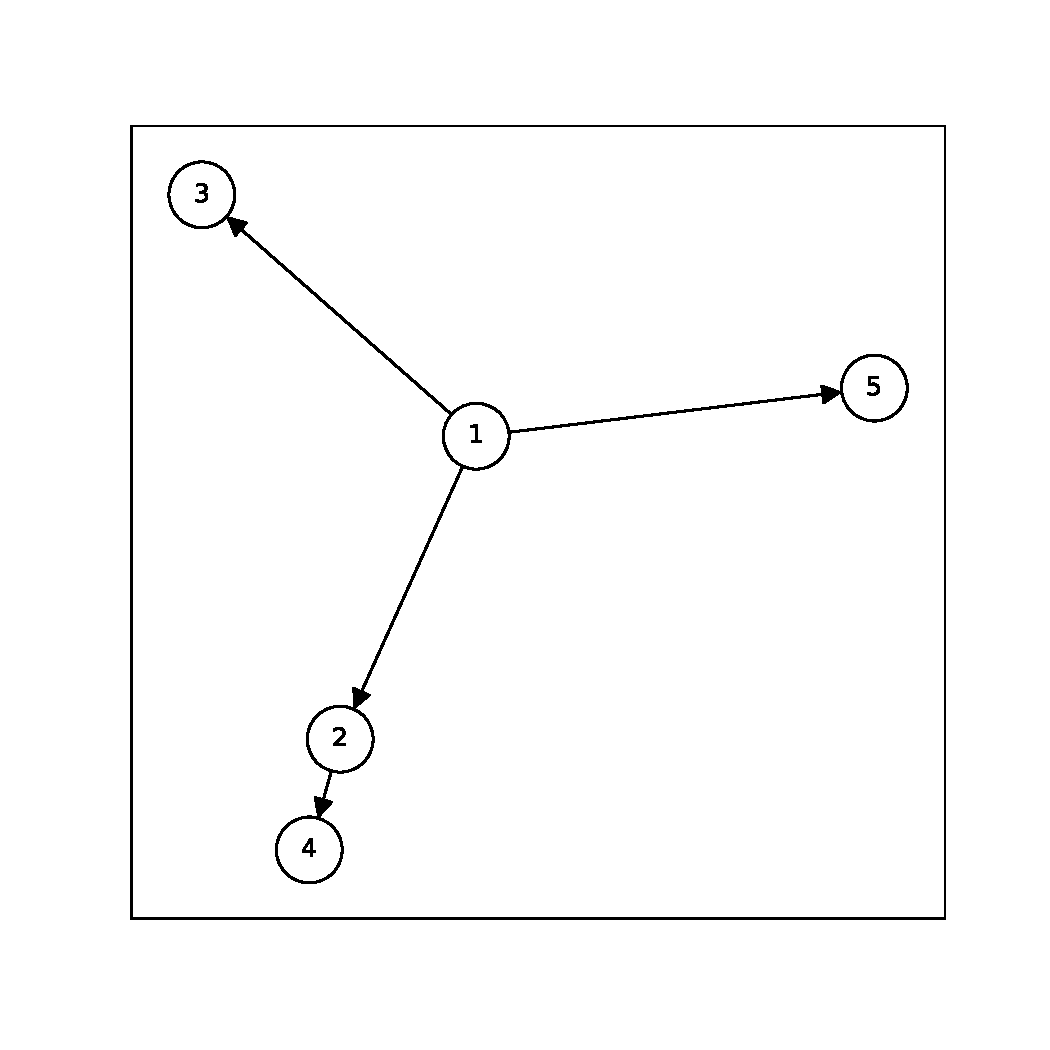
\includegraphics[width=\linewidth]{ ./figures/dageg.pdf}\caption{ Example of a DAG $\mathbb{G}=(\mathbb{V},\mathbb{E})$ with $\mathbb{V} = \{1,2,3,4,5 \}$ and $\mathbb{E} = \{(1,2),(1,3),(1,5),(2,4) \}$. Here $PA_{\mathbb{G}}(2)=\{1\}$, $DS_{\mathbb{G}}(2)=CH_{\mathbb{G}}(2)=\{1\}$, $ND_{\mathbb{G}}(2)=\{3,5\}$} \end{marginfigure} 
 \begin{marginfigure} 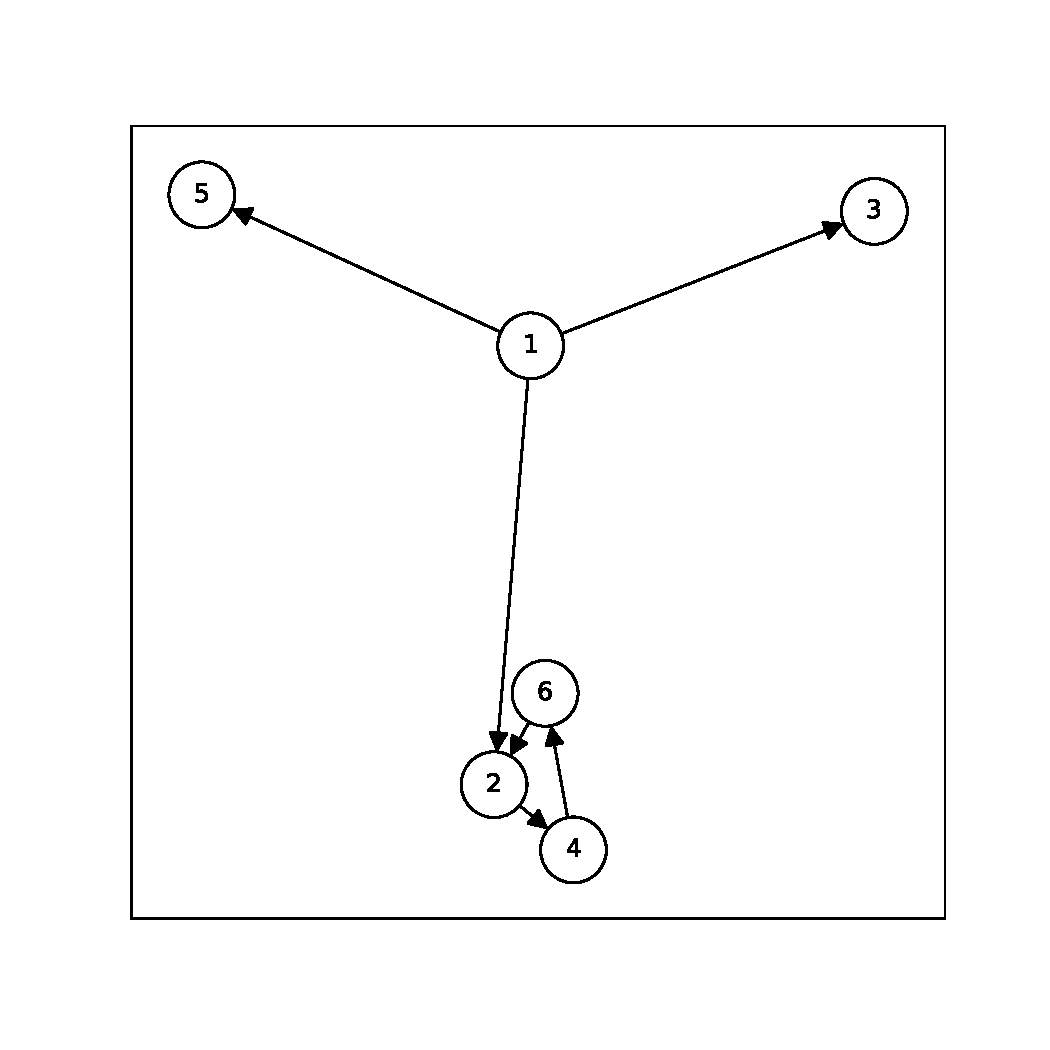
\includegraphics[width=\linewidth]{ ./figures/dagneg.pdf}\caption{ This graph is not a DAG since there is a cycle} \end{marginfigure} 

\begin{definition}[DAGs]\label{dagdef}
    A Directed Acyclic Graphic (DAG) is a directed graph $\mathbb{G} = (\mathbb{V},\mathbb{E})$ which has no cycles.
\end{definition}

Let $\mathbb{G} = (\mathbb{V},\mathbb{E})$ be a graph. We then have the following definitions. A node $u \in \mathbb{V}$ is a \textbf{parent} of another node $u \in \mathbb{V}$ if $(u,v) \in \mathbb{E}$, in this case we also say $v$ is a \textbf{child} of $u$. If there is an edge $(u,v) \in \mathbb{E}$ or $(v,u)\in \mathbb{E}$ we say the nodes $u$,$v$ are \textbf{adjacent}. A sequence of nodes $(u_1,...,u_k)$ , $k\geq 2$ such that $(u_i,u_{i+1}) \in \mathbb{E}$ is called a path between $u_1$ and $u_k$. In this case, we say $u_1$ is an \textbf{ancestor} of $u_k$ and $u_k$ is a \textbf{descendant} of $u_1$. If we have a node $v$ that is not a descendant of a node $u$ we say $v$ is a \textbf{non-descendant} of $u$.


For any node $u \in \mathbb{V}$ we denote $PA_{\mathbb{G}}(u)$, $CH_{\mathbb{G}}(u)$, $DS_{\mathbb{G}}(u)$, $ND_{\mathbb{G}}(u)$ to be set of parents, children, descendants and non-descendants of $u$ respectively.

\end{definition}

Throughout this work we let $[p]=\{1,...,p\}$ be the set of nodes for DAGs, and $\subset$ denotes the subset relation, not the proper subset.




Since we a working with discrete probability distributions, we introduce the (open) probability simplex as the space of all possible probability distributions over a set of discrete variables \(X_1,...,X_p\) whose outcomes are elements of \(\mathcal{X}=\prod_{i=1}^p \mathcal{X}_i\).

\begin{definition}[Probability simplex]\label{probsimplex}
Given a finite set $\mathcal{X}$, The probability simplex on this set is \\ $\Delta_{|\mathcal{X}|-1} = \{ (f_x \, : x \in \mathcal{X}) \in \mathbb{R}^{|\mathcal{X}|} \, : \, \forall x \in \mathcal{X} \; f_x > 0, \, \sum_{x\in \mathcal{X}}f_x =1\}.$
\end{definition}

Each point in the probability simplex corresponds to a joint distribution over \((X_1,...,X_p)\), and our interest mainly lies to the subset of of this space which are connected to structures we can use to model causal relations.


An important concept when relating DAGs to distributions is that of conditional independence, which we define below.
\begin{definition}[Conditional Independence]\label{def:cirel}
Let  $\mathbb{P}$ be a distribution with variables $X_1,...,X_p$. Given non-empty subsets $A,B \subset [p]$ and a (possibly empty) subset $S \subset [p]$ such that $\mathbb{P}(X_B, X_S)>0$ and $A \cap B \cap S = \{\}$, we say the variables $X_A$ and $X_B$ are conditionally independent given $S$, (denoted $(X_A\indep_{\mathbb{P}} X_B \,|\, X_S)$) if $\mathbb{P}(X_A, \,|\,X_B, X_S) = \mathbb{P}(X_A \, |\, X_S)$ holds for all possible outcomes of $X_A,X_B,X_S$.
\end{definition}

The conditional independence statement  \footnote{Given a set $A \subset [p]$, $X_A = \{X_a \}_{a \in A}$}   \((X_A \indep_{\mathbb{P}} X_B \,|\,X_S)\) can be viewed as a ternary relation on \(X_A,X_B,X_S\), and is called a Conditional Independence (CI) relation. This relation formalizes the concept of \(X_B\) and \(X_A\) not providing any information for the other when we have observed \(X_S\), which is to say, if we already know \(X_S\), knowing \(X_B\) does not change the probabilities for \(X_A\), and vice versa.


Using this we can now define the local Markov property which relates distributions to DAGs based on the CI relations encoded by them. As the CI relations have a natural causal interpretation, the local Markov property provides a foundation to relate data generating distributions to DAG representations of a causal system.


\begin{definition}[Local Markov property]\label{thm:localmarkovdag}
Let $\mathbb{G}$ be a DAG with nodes $[p]$. A probability distribution $\mathbb{P}$ satisfies the local Markov property with respect to $\mathbb{G}$ if for each node $i \in [p]$, the variable representing that node, $X_i$ is independent of its non-descendants when conditioned on its parents, formally, $(X_i \indep_{\mathbb{P}} X_{ND_{\mathbb{G}}(i)}\,|\,X_{PA_{\mathbb{G}}(i)})$.
\end{definition}

This formalizes the fact that in order to computationally generate data from a DAG \(\mathbb{G}\), the value of each variable \(X_i \in \mathcal{X}_i\) depends only on the values of the outcomes of its parents in \(\mathbb{G}\). This means that for a (discrete) distribution \(\mathbb{P}\) with \(p\) variables satisfying the Local Markov property, the distribution can be encoded with \(p\) probability tables which give the probabilities for each \(X_i\) taking a value when conditioned on all possible outcomes of its parents. From a storage perspective, this means we have to store \(\sum_{i=1}^p |\mathcal{X}_i| |\prod_{j \in PA_{\mathbb{G}}(i)}\mathcal{X}_j |\) values. This is significantly smaller than having to store all possible probability values which would require  \(\sum_{i=1}^p |\mathcal{X}_i||\prod_{i=1}^p \mathcal{X}_i|\) values. For binary variables assuming \(d\) parents for each variable, this is the difference between \(p2^{d+1}\) and \(p2^{p+1}\).


For the purposes of this thesis, it is worth introducing the Ordered Markov property which uses the concept of a linear ordering.  \footnote{For a DAG \mathbb{G} with $p$ nodes a linear ordering is an ordering of the nodes that respects the directions in $\mathbb{G}$, that is each node $i$ always comes after each $j \in PA_{\mathbb{G}}(i)$. It is also called a topological ordering, and later on we will use this ordering as a causal ordering for events.} 

\begin{definition}[Ordered Markov Property]\label{orderedmarkov}
Let $\mathbb{G}$ be a DAG and $\pi = \pi_1 \cdots \pi_p$ a causal ordering of $\mmathbb{G}$. A probability distribution $\mathbb{P}$ satisfies the Ordered Markov property with respect to $\mathbb{G}$ if we have $(X_i \indep_{\mathbb{P}} X_{\{1,...,i-1 \} \textbackslash PA_{\mathbb{G}}(i)}\,|\, X_{PA_{\mathbb{G}}(i)})$.
\end{definition}

A distribution \(\mathbb{P}\) satisfying the local Markov property with respect to a DAG \(\mathbb{G}\) is equivalent to that distribution satisfying the ordered Markov property with respect to \(\mathbb{G}\) and a linear ordering of \(\mathbb{G}\).


An important notion in DAGs is that of d-separation and blocked paths.
  \footnote{\baselineskip \baselineskip Recall that a path between 2 nodes is any sequence of edges connecting them irrespective of edge direction.} .


\begin{definition}[Blocked path]\label{bpath}

Given a DAG $\mathbb{G}$, and a path between nodes $i,j \in \mathbb{V}$, we say the \textbf{path is blocked} by a (potentially empty) set of nodes $S$ if either of the following hold:
\begin{itemize}
\item Along the path there is a triple of nodes $(x,s,y)$ such that $x \rightarrow s \rightarrow y$, $x \leftarrow s \leftarrow y$, or $x \leftarrow s \rightarrow y$ with $s \in S$
\item Along the path there is a triple of nodes $(x,s,y)$ such that $x \rightarrow s \leftarrow y$ such that $s \notin S$ and no descendants of $s$ are in $S$.
\end{itemize}

\end{definition}


\begin{definition}[d-separation]\label{def:dsep}

Given a DAG $\mathbb{G}$,  two (non-empty) sets of nodes $X,Y$ are \textbf{d-separated} by a (potentially empty) set of nodes $S$ in $\mathbb{G}$, denoted $(X\indep_{\mathbb{G}}Y\,|\,S)$ if all paths between every node in $X$ and every node in $Y$ are blocked by $S$. 

\end{definition}

 \begin{marginfigure} 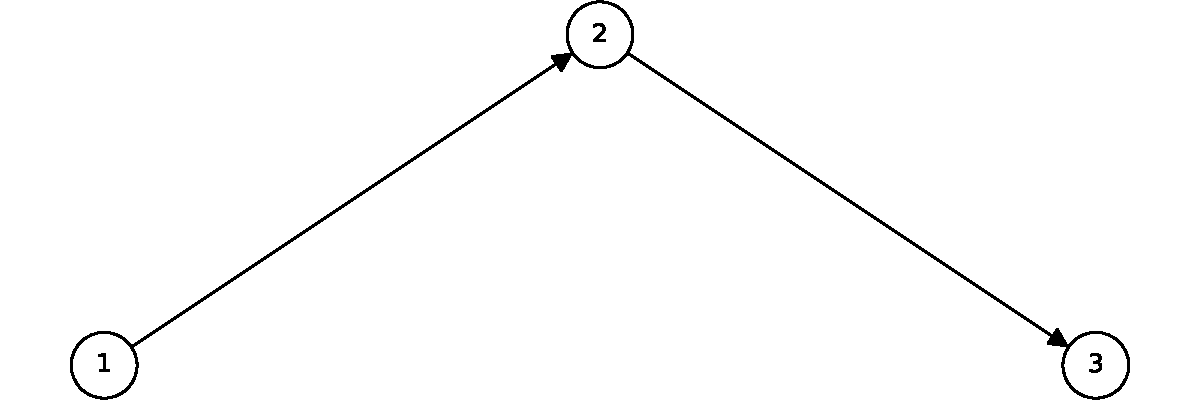
\includegraphics[width=\linewidth]{ ./figures/chainl.pdf}\caption{ Chain} \end{marginfigure} 

 \begin{marginfigure} 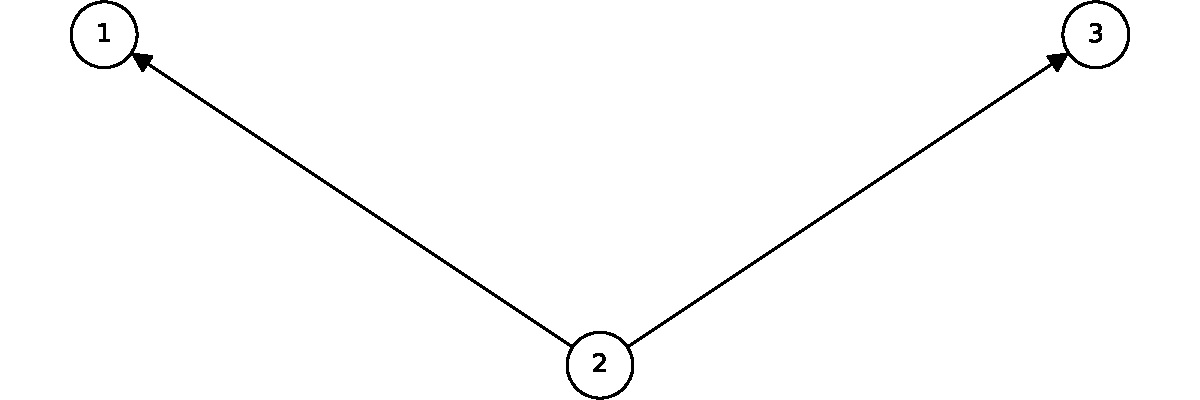
\includegraphics[width=\linewidth]{ ./figures/fork.pdf}\caption{ Fork/Common cause} \end{marginfigure} 
 \begin{marginfigure} 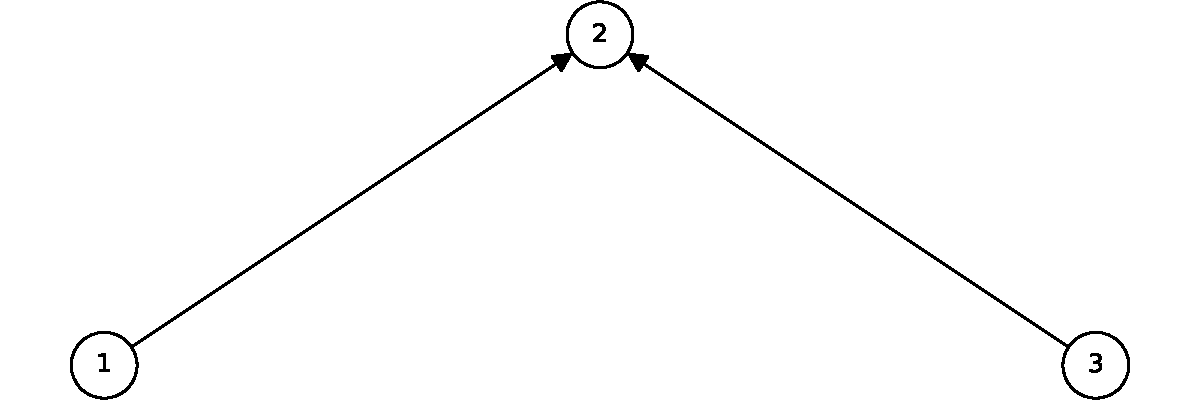
\includegraphics[width=\linewidth]{ ./figures/collider.pdf}\caption{ V-structure/ Collider/Immorality} \end{marginfigure} 


The notion of d-separation relates DAGs to probability distributions from the following theorem.
\begin{definition}[Global Markov property]\label{thm:dagci}

Given a distribution $\mathbb{P}$ that satisfies the local Markov property with a DAG $\mathbb{G}$, we have that for any (non-empty) sets $A,B$ and (possibly empty) set $S$, $(X_A \indep_{\mathbb{G}} X_B \,|\,X_S) \implies (X_A \indep_{\mathbb{P}} X_B \,|\, X_S)$


\end{definition}

An important result states that the above notions are indeed equivalent \cite{duarte-2020-algeb-geomet}.

\begin{theorem}[Markov theorems for DAGs]\label{thm:markovdag}
Given a distribution $\mathbb{P}$ over $X_1,...,X_p$ and a DAG $\mathbb{G}$ over $p$ nodes, the following are equivalent

\begin{itemize}
\item $\mathbb{P}$ is Markov to $\mathbb{G}$ i.e. $\mathbb{P}(X_1,...,X_p) = \prod_{i=1}^p \mathbb{P}(X_i \, |\, X_{PA_{\mathbb{G}}(i)})$
\item $\mathbb{P}, \mathbb{G}$ satisfy the local Markov property
\item $\mathbb{P}, \mathbb{G}$ satisfy the ordered Markov property
\item $\mathbb{P}, \mathbb{G}$ satisfy the global Markov property
\end{itemize}

\end{theorem}


If \(\mathbb{P}\) satisfies the local Markov property with respect to \(\mathbb{G}\) and has a probability density with respect to a product measure, we say \(\mathbb{P}\) is Markov with respect to \(\mathbb{G}\), or equivalently, \(\mathbb{G}\) is an Independence map (I-MAP) of \(\mathbb{P}\) \cite{lauritzen-1996-graph}.

Thus, DAGs can be seen as structures that encode Conditional Independence (CI) relations. More importantly, d-separation encodes the complete set of CI relations satisfied by all distributions Markov to a DAG, i.e. distributions that are Markov to a DAG \(\mathbb{G}\) \textbf{and} satisfy \textbf{exactly} the CI relations encoded by d-separation exist \cite{meek-1995-stron-compl,geiger-1990-ident-indep}.

It is also possible to have 2 DAGs that encode the same CI relations, in which case we say that they are both in the same Markov Equivalence Class (MEC), and we say they are Markov Equivalent. MECs can be characterized by the following theorem \cite{verma-2013-equiv-causal-model}.

\begin{theorem}[Characterization of MECs of DAGs]\label{thm:vermapearl}
Two DAGs $\mathbb{G}_1$ and $\mathbb{G}_2$ are Markov Equivalent if and only if they have the same skeleton (underlying undirected edges) and v-structures, where a v-structure is a triple of nodes $(i,j,k)$ with edges $i \rightarrow j \leftarrow k$ and $i,k$ do not share an edge.
\end{theorem}

For example, the Chain and Fork graphs from the previous page belong to the same Markov Equivalence class.

\section{Causal Discovery Algorithms for DAGs}
\label{sec:org93a8b8f}

Theorem \ref{thm:markovdag} suggests that we can make use of CI testing on a distribution \(\mathbb{P}\) to learn a DAG \(\mathbb{G}\). However, the distribution \(\mathbb{P}\) may contain CI relations not encoded in the DAG, hence we make the following assumption.

\begin{definition}[Faithfulness]\label{def:faithfulness}

A probability distribution $\mathbb{P}$ is faithful to a DAG $\mathbb{G}$ if it entails only the CI relations encoded by the d-separations in the DAG.

\end{definition}

Under the faithfulness assumption, the global Markov property holds both ways. It should be noted that faithful distributions exist \cite{meek-1995-stron-compl}, and the set of distributions that are not faithful to a DAG \(\mathbb{G}\) have measure \(0\) \cite{uhler-2013-geomet-faith}, which suggets that in theory this is not a very restrictive assumption.



One of the first practical algorithms which make use of the theory above is the PC algorithm, \cite{spirtes-2000-causation-prediction-search,kalisch-2007-estim-high} which is a constraint-based causal discovery algorithm that relies on the characterization of DAGs in Theorem \ref{thm:vermapearl} and the faithfulness assumption to find a DAG in the MEC of the true causal DAG. The algorithm starts from a complete graph and runs conditional independence tests to first find the DAG skeleton, then its v-structures, then proceeds to direct the edges whenever possible. The output of the PC algorithm is a Completed Partially Directed Acyclic Graph (CPDAG) \cite{meek-1995-causal-infer}, which acts as a representation for the Markov Equivalence class. A Partially Directed Acyclic Graph (PDAG) is a graph where some edges are directed and some are undirected and there is no cycle in the direction of the directed edges and any direction of the undirected edges. A PDAG a is Complete PDAG (CPDAG) if every directed edge exists also in every DAG in the Markov Equivalence class of the DAG and for every undirected edge between nodes \(i,j\) there exists a DAG with the edge \(i \rightarrow j\) and a DAG with \(j \rightarrow i\) in the equivalence class. CPDAGs are also sometimes called essential graphs \cite{andersson-1997-charac-markov}.






\section{Limitations of using DAGs}
\label{sec:org9d90bb0}
DAGs are a simple and informative structure for causal discovery, however their ability to only encode CI relations is a limitation. This is because the CI relation  \((X_A \indep_{\mathbb{P}} X_B \,|\, X_S)\) implies that \(X_A\) and \(X_B\) are independent for all possible outcomes of \(X_S\), which in some cases might be too strong of an assumption. A generalization of such relations is Context-Specific conditional Independence (CSI) relations  \footnote{We will sometimes refer to these as context-specific independence relations.} , defined below.
\begin{definition}[Context-Specific Conditional Independence]\label{def:csirel}
Let  $\mathbb{P}$ be a distribution with variables $X_1,...,X_p$ with a state space $\mathcal{X} = \prod_{i=1}^p \mathcal{X}_i$. Given (non-empty) subsets $A,B \subset [p]$ and (possibly empty) subsets $S,C \subset [p]$ and $x_C \in \prod_{i \in C}\mathcal{X}_i $ such that $\mathbb{P}(X_B, X_S, X_C = x_C)>0$ and $A \cap B \cap S \cap C = \{\}$, we say the variables $X_A$ and $X_B$ are conditionally independent given $S$, in the context $X_C=x_C$ (denoted $(X_A\indep_{\mathbb{P}} X_B \,|\, X_S, X_C=x_C)$) if $\mathbb{P}(X_A \,|\,X_B, X_S,X_C=x_C) = \mathbb{P}(X_A \, |\, X_S,X_C=x_C)$ holds for all possible outcomes of $X_A,X_B,X_S$.
\end{definition}


In the next chapter we introduce Context-Specific Trees (CStrees) which can encode such relations, whilst still allowing for an intuitive representation as a sequence of DAGs.


 \newpage 

\chapter{Causal Discovery with Context-Specific Trees}
\label{sec:org52fa879}
One intuition is that to capture context specific relations one needs to make use of a structure that explicitly represents separate outcomes of a distribution. In high school some might have encountered the use of trees to model small probabilistic systems, and they fully include all possible outcomes involved, and serve as an important tool to compute probabilities for relevant events. As we will see in this chapter, this is a good way to approach the problem of encoding context-specific information as well.

\section{Context Specific Trees (CStrees)}
\label{sec:orge7cfa85}
Before defining CStrees we start by defining staged trees, which contain CStrees as a subclass. Both of these are rooted trees.  \footnote{A rooted tree $\mathbb{T} = (\mathbb{V},\mathbb{E})$ is a directed graph whose skeleton is a tree and there exists a unique node $r$ such that $PA_{\mathbb{T}}(r) = \{\}$ which is called the root.} 
   \begin{definition}[Staged trees]
   Let $\mathbb{T} = (\mathbb{V},\mathbb{E})$ be a rooted tree, $\mathbb{L}$ a finite set of labels for the edges, and $\theta : \mathbb{E} \rightarrow \mathbb{L}$ a labelling of the edges. Let $E_{\mathbb{T}}(v) = \{v \rightarrow w \in \mathbb{E} \,:\, w \in CH_{\mathbb{T}}(v) \}$,   i.e. the set of edges coming out of $v$ in $\mathbb{T}$. The pair $(\mathbb{T}, \theta)$ is a staged tree if 
\begin{itemize}
\item  $\forall v \in \mathbb{V}$ we have |$\theta(E_{\mathbb{T}}(v))$| = |$E_{\mathbb{T}}(v)$|.
\item $\forall v,w \in \mathbb{V}$ we have that both $\theta(E_\mathbb{T}(v))$ and $\theta(E_\mathbb{T}(w))$ are either equal or disjoint.
\end{itemize}
\end{definition}

This can be thought of as a probability tree where each edge represents a probability value, and the probabilities coming out of all edges from any given node sum to 1. More formally, first define the space of canonical parameters of the staged tree \((\mathbb{T},\theta)\) as

$\Theta_{\mathbb{T}} = \{  x\in \mathbb{R}^{|\mathbb{L}|} \, : \, \forall e \in \mathbb{E}, x_{\theta(e)}\in (0,1), \forall v \in \mathbb{V}, \, \sum_{e \in E_{\mathbb{T}}(v)} x_{\theta(e)}=1 \}$.

Given the probability simplex \(\Delta_{|\mathcal{X}|-1}\) and letting \(\mathbf{i}_{\mathbb{T}}\) be the set of all leaves of the staged tree \(\mathbb{T}\)  the staged tree model is defined as below.


\begin{definition}[Staged tree models]\label{def:stagedtreemodel}
The staged tree model $\mathbb{M}_{(\mathbb{T},\theta)}$ is the image of the map $\varphi_\mathbb{T} \, : \, x \rightarrow f_v := $ $\Big($ $\prod_{e \in E_{\mathbb{T}(\lambda(v))} x_{\theta(e)}$ $\Big)_{v \in \mathbf{i}_{\mathbb{T}}}$
\end{definition}
 \begin{marginfigure} 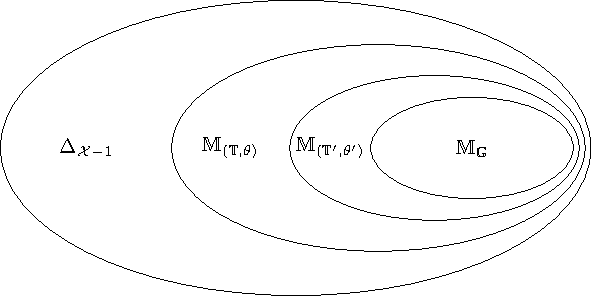
\includegraphics[width=\linewidth]{ ./figures/modelhierarchy.pdf}\caption{ Hierarchy of models on $\mathcal{X}$ that we are concerned with, the most general space of models being probability simplex since it contains all distributions on $\mathcal{X}$, followed by the space of staged tree models $\mathbb{M}^*_{(\mathbb{T},\theta)}$, the space of CStree models $\mathbb{M}^*_{(\mathbb{T}', \theta)}$ then DAG models $\mathbb{M}^*_{\mathbb{G}}$. More general models can explain more datasets whilst simpler models can often be easier to work with.} \end{marginfigure} 
Here, \(\lambda(v)\) denotes the unique path from the root to \(v\). Thus, given variables \(X_1,...,X_p\), and a causal ordering \(\pi\) \footnote{A causal ordering is an ordering of the $p$ variables used to construct the levels of the CStree.} , the staged tree for this pair with levels  \footnote{The $k^{th}$ level of a rooted tree, $L_k$, is the set of nodes such that the unique path from each node in $L_k$ to the root consists of $k$ edges.}  \(L_1,...,L_p \sim X_{\pi_1},...,X_{\pi_p}\), each path from the root to the leaf defines a sequence of events \(x_1, x_1x_2, ...,x_1\cdots x_p\) where \(x_i \in \mathcal{X}_{\pi_i}\). Since for the edge  \(e = ((x_1\cdots x_k), (x_1\cdots x_kx_{k+1}))\) we have \(x_{\theta(e)} = \mathbb{P}(x_{k+1}\,|\, x_1\cdots x_k)\), the product in Definition \ref{def:stagedtreemodel} does indeed result in \(\mathbb{P}(v_1,...,v_p)\) for each \(v \in \textbf{i}_{\mathbb{T}}\) by the chain rule in probability.  \footnote{The chain rule in probability states $\mathbb{P}(X_1 ,...,X_p) = \mathbb{P}(X_p \; |\; X_{p-1},...,X_1)\mathbb{P}(X_{p-1} \; | \; X_{p-2},...,X_1 )\\ \cdots \mathbb{P}(X_2|X_1)\mathbb{P}(X_1).} 

The important characteristic of staged trees are their stages. 

\begin{definition}[Stages]

Given a staged tree $(\mathbb{T},\theta)$, we say two nodes $v,w$ are in the same stage if and only if  $\theta(E_\mathbb{T}(v)) = \theta(E_\mathbb{T}(w))$

\end{definition}


Stages are represented by colours, and when a stage contains a single node, it is coloured white. Staged tree models generalize DAG models, i.e. distributions represented by DAGs, however they are perhaps too general, in the sense that despite allowing for the representation of context-specific information, they do not admit a intuitive representation of the causal structure. This creates the need for a structure that generalizes DAG models \textbf{and} admits an intuitive representation. The recently proposed subclass of staged trees, known as CStrees allow for this.

\begin{definition}[CStrees]\label{def:cstree}
Let $\mathcal{X}_i$ denote the state space of some variable $X_i$ with $\mathcal{X} = \Pi_{i=1}^p \mathcal{X}_i$, and $(\mathbb{T},\theta)$ be a staged tree with levels $L_1,...,L_p$ corresponding to variables $X_{\pi_1},...,X_{\pi_p}$ where $\pi = \pi_1...\pi_p$ is the causal ordering of the variables.  
A CStree is a staged tree $(\mathbb{T}, \theta)$ where each level of the tree corresponds to some variable and  such that 
\begin{itemize}
\item It is compatibly labeled, i.e. $\forall x_{\pi_k} \in \mathcal{X}_{\pi_k}$ we have $\theta(x_{\pi_1}...x_{\pi_{k-1}}\rightarrow x_{\pi_{k-1}}x_{\pi_k}) = \theta(y_{\pi_1}...y_{\pi_{k-1}}\rightarrow y_{\pi_{k-1}}x_{\pi_k})$ whenever $x_{\pi_1}...x_{\pi_{k-1}}$ and $y_{\pi_1}...y_{\pi_{k-1}}$ are in the same stage.
\item (\textbf{CStree property}) Each stage $S_i \subset L_k$ of the tree has a fixed context, i.e. $\exists C_i \subset [k]$ and the fixed outcome $x_{C_i} \in \mathcal{X}_{C_i}$, where the stages contain nodes generated from taking the union over the variables beside those in $C_i$, i.e. if $Y_i = [k] \textbackslash C_i$ then $S_i = \bigcup_{x_{Y_i} \in \mathcal{X}_{Y_i}} \{x_{C_i}x_{Y_i} \}$.
\end{itemize}
\end{definition}



Given a CStree \(\mathbb{T}\) and a causal ordering \(\pi\), each node in level \(L_k\) corresponds to an outcome of the sequence of variables \(X_{\pi_1},...,X_{\pi_k}\). Each edge coming into each node in \(L_k\) is of the form \((x_1\cdots x_{k-1},x_1\cdots x_k)\) represents \(P(x_{k}|x_1 \cdots x_{k-1})\), which is also the value of the parameter associated to this edge. Suppose we fix a node \(n = a_1\cdots a_k \in L_k\). Each edge coming out of \(n\) gives the probabilities for the variable in the next level \(L_{k+1}\), conditioned on the context \((X_{\pi_1}=a_1,...,X_{\pi_k}=a_k)\). Thus, we can view this node \(n\) as representing the distribution \(\mathbb{P}(X_{\pi_{k+1}}\,|\, X_{\pi_1}=a_1,...,X_{\pi_k}=a_k)\). This is an important view which we will make use of when testing for context-specific independence in the algorithms throughout this paper. We show an example of a CStree and a staged tree that is not a CStree below.



\begin{figure}[!h]\label{fig:cstreestagedtree}
   \begin{floatrow}
\ffigbox{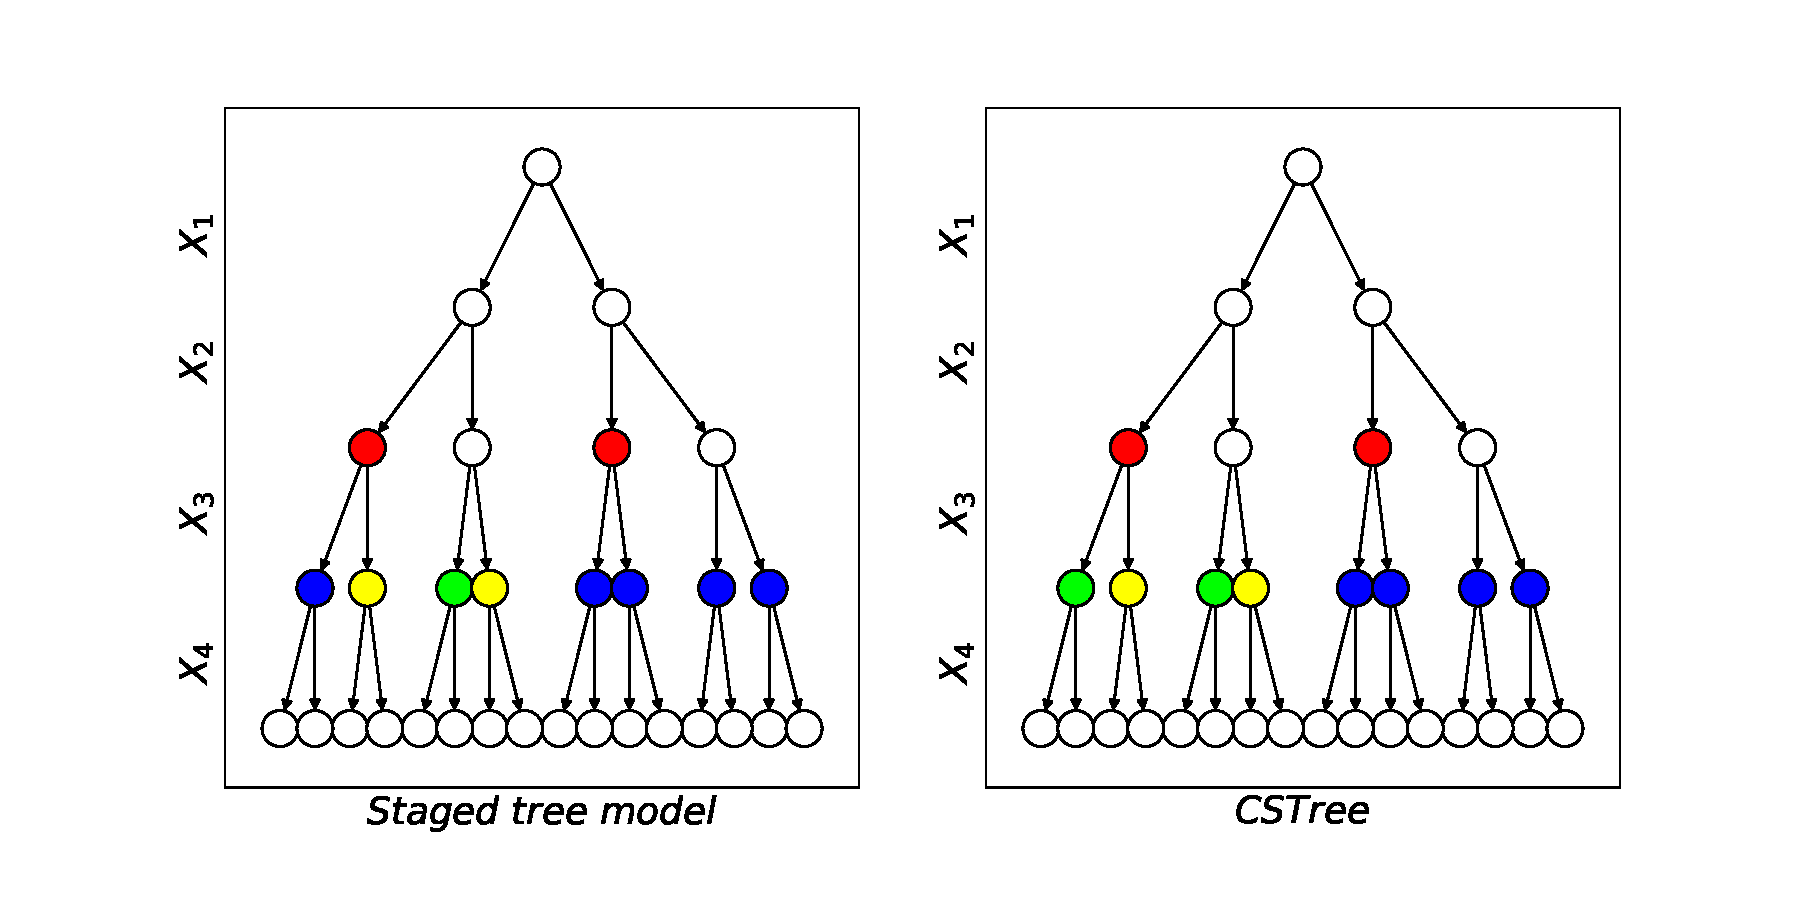
\includegraphics[width=0.95\linewidth]{figures/cstreestagedtree.pdf}}%
\caption{Example of a staged tree model that is not a CStree (left) and a CStree (right) for binary variables $X_1,X_2,X_3,X_4$ in that causal ordering.}
        
   \end{floatrow}
\end{figure}

Both staged trees in Figure \ref{fig:cstreestagedtree} represent 4 binary variables \(X_1,X_2,X_3,X_4\) taking values in \(\{0,1\}\) in that causal order. Suppose each edge to the left corresponds to the outcome \(0\) and the other corresponds to \(1\). In this case, the left edge coming out of the root represents \(\mathbb{P}(X_1 = 0)\) and the right edge coming out the root represents \(\mathbb{P}(X_1 = 1)\). The nodes represent distributions conditioned on the context unique to them. For example, the left-most red node in both trees represent \(\mathbb{P}(X_3 \,|\, X_2=0, X_1=0)\). The tree on the right is a CStree because each of the nodes in the non-singleton stages, which are represented by a non-white colour, share exactly one fixed context. For example, the stage corresponding to the blue nodes in the tree on the right (the CStree) corresponds to the contexts \((X_1=1, X_2=0, X_3=0), (X_1=1, X_2=1, X_3=1), (X_1=1, X_2=1, X_3=0), (X_1=1, X_2=1, X_3=1)\). The common context for this stage is  \((X_1=1)\). Meanwhile, for the tree on the left, the stage corresponding to the blue nodes only share the empty context, meaning all nodes in level 3 must correspond to the stage with the empty context for it to be a CStree - this is however not the case since there are nodes in level 3 which correspond to the yellow and green stages, thus not part of the blue stage. 


A CStree encodes Context-Specific Conditional Independence (CSI) relations according to the following lemma \cite{duarte-2021-repres-contex}.


\begin{lemma}[CStrees and CSI relations]\label{lem:cstreecsi}

Let $\mathbb{T} = (\mathbb{V},\mathbb{E})$ be a CStree with levels $X_1,...,X_p \sim L_1,...,L_p$ and stages $S_1,...,S_m$. Then for any $\mathbb{P} \in \mathbb{M}_{(\mathbb{T},\theta)}$ and $S_i \subset L_{k-1}$, $\mathbb{P}$ entails the CSI relation $(X_k \indep_{\mathbb{P}} X_{[k-1] \textbackslash C_i} \, | \, X_{C_i} = x_{C_i})$ where $X_{C_i}=x_{C_i}$ is the context fixed by the stage $S_i$.

\end{lemma}

The CSI relations from the CStrees look similar to the CI relations from the ordered Markov property. The difference is that the CStree encodes independence of \(X_k\) with all the variables preceding it in the causal ordering when conditioned on a context, compared to the ordered Markov property which contains the variables which represent the parents of \(k\) in the conditioning set. Thus, CStrees can be thought of as a relaxation of DAG models via a relaxation of the ordered Markov property, where we condition on the more general scenario of contexts, rather than variables. 


One question that arises is how many CStrees are there for a given system of variables \(X_1,...,X_p\) taking values in \(\mathcal{X}_1,...,\mathcal{X}_p\). The authors of the original CStree paper \cite{duarte-2021-repres-contex} provide a closed form expression for the number of CStrees on \(p\) binary variables, alongside a table comparing the number of DAGs (sequence A003024 in oeis.org), CStrees and comptabily labeled staged trees, which we include below in Table \ref{tab:org087338d}. A closed form expression for general CStrees remains to be discovered.

\begin{table}[htbp]
\caption{\label{tab:org087338d}Number of DAGs, CStrees and compatibly labeled staged trees on \(p\) binary variables.}
\centering
\begin{tabular}{r|r|r|r}
\hline
\(p\) & DAGs & CStrees & Compatibly labeled staged trees\\
\hline
1 & 1 & 1 & 1\\
2 & 3 & 4 & 4\\
3 & 25 & 96 & 180\\
4 & 543 & 59136 & 2980800\\
5 & 29281 & 26466908160 & 156196038558888000\\
\end{tabular}
\end{table}





\section{Learning CStrees from observed data}
\label{sec:org44f8475}
Given a system of variables \(X_1,...,X_p\), we would first need a causal ordering \(\pi_1 \cdots \pi_p\) in order to construct a CStree for these variables. Since CStrees encode CSI relations, they can also encode CI relations, which means we can generate a CStree from a DAG. The following proposition formalizes this notion \cite{duarte-2020-algeb-geomet}.

\begin{proposition}[CStrees corresponding to DAGs]\label{prop:dagandcstree}
A compatibly labeled staged tree $\mathbb{T}$ with causal ordering $\pi_1 \cdots\pi_p$, levels $L_1,...,L_p$ corresponding to variables $X_{\pi_1},...,X_{\pi_p}$ encodes the same CI relations as some DAG $\mathbb{G}$ if and only if for any topological ordering of $\mathbb{G}$, $\forall k \in [p-1]$, the level $L_k$ has its nodes partitioned into stages where the context for each stage is an element of the Cartesian product of the parents of $X_{\pi_{k+1}}$ in $\mathbb{G}$.
\end{proposition}

We describe the computational procedure to generate a CStree \(\mathbb{T}\) from a DAG \(\mathbb{G}\) below, assuming that we are given a causal ordering of \(\mathbb{G}\).  \footnote{\textsc{Parents} is a function that takes a graph and a node and returns the parents of that node in the graph; \textsc{CartesianProduct} takes a set of variables and returns the cartesian product of these variables i.e. all possible values they can take.} .



\begin{algorithm}[H]
\label{alg:dagtocstree}
      \SetAlgoLined
      \KwIn{A DAG $G$, causal ordering $O$}
      \KwOut{CStree $T$ with ordering $O$ and stages $S$ defined by $G$}
      $T \gets$ Empty staged tree with ordering $O$\;
      $S \gets$ Empty List\;
       \For{$k$ in $|O|-1$}{
        $v \leftarrow O[k+1]$ \;
	$T.add\_level(v)$\;
	$pars \leftarrow \;  \textsc{Parents}(G, v)$\;
	$contexts \leftarrow$ \textsc{CartesianProduct}($pars$)\;
	$stages\_k \gets$ Empty Dictionary\;
	\For{$c$ in $contexts$}{
	$stages\_k[c] \leftarrow$ [nodes in level $k$ where $c$ is a subcontext]\;
	}
	$S.append(stages\_k)$\;
       }
       \caption{\textsc{DagToCStree}\\Constructing a CStree from a DAG}
       \KwRet{$T, S$}
      \end{algorithm}

Algorithm \ref{alg:dagtocstree} above does not necessarily need a causal ordering. This is because given a DAG we can perform a topological sort on it to get one, for which efficient algorithms exist \cite{tarjan-1976-edge-disjoin}.

\begin{theorem}\label{thm:dagtocstreecorrectness}
Given variables $X_1,...,X_p$ taking values in $\mathcal{X}=\prod_{i=1}^p \mathcal{X}_i$ , Algorithm \ref{alg:dagtocstree} is correct i.e. it takes a DAG and returns the corresponding CStree in $\mathcal{O}(d^{2p})$ time and $\mathcal{O}(d^p)$ space where $d = \max_{i \in [p]} |\mathcal{X}_i|$.
\end{theorem}

\textit{Proof:
	For correctness, at each level $L_k$, the non-singleton stages are created for the contexts fixed by the outcomes of the parents of $X_{\pi_{k+1}}$ thus by Proposition \ref{prop:dagandcstree} the tree is still a CStree. Since the staging process at each level only creates non-singleton stages of nodes within that level, and we go over each level except the last level which always contains singleton stages (one for each outcome of $\mathcal{X}$), the stages $S$ lead to $T$ being a CStree. For time complexity, the worst case scenario is for the fully connected DAG, assuming the ordering $12\cdots p$, node $i$ has $i-1$ parents. This however results in a CStree with no non-singleton stages. Thus we look at the scenario where node $i$ has $i-2$ parents. At the level for the variable representing node $i$, the variable $contexts$ in Algorithm \ref{alg:dagtocstree} which is all the elements of the the Cartesian product of values the parents take, has $|\prod_{j=1}^{i-2} \mathcal{X}_j|$ elements. For each element in this Cartesian product which fixes the context for the stage, we have to loop over all nodes in level $i$ and to store the nodes for that stage, and level $i$ has $|\prod_{j=1}^i \mathcal{X}_j|$ nodes. Thus the loop for level $i$ takes $|\prod_{j=3}^{i-2} \mathcal{X}_j ||\prod_{j=1}^i \mathcal{X}_j| $ where the indexing starts at 3 for the first term since the parent sets are non-empty starting from node 3. Since we have $p$ levels, ignoring the first 2 since their variables have no parents, we have}

	\begin{align*}\sum_{i=3}^p |\prod_{j=3}^{i-2} \mathcal{X}_j ||\prod_{k=1}^i \mathcal{X}_k| < \sum_{i=1}^p |\prod_{j=1}^i |\mathcal{X}_j||\prod_{k=1}^i |\mathcal{X}_k|< \sum_{i=1}^p \prod_{j=1}^i d \prod_{k=1}^i d 
	\end{align*}

\textit{where $d = \max_{i \in [p]} |\mathcal{X}_i|$. This sum then becomes }
\begin{align*}
\sum_{i=1}^p d^{2i}  = \frac{d^2 (d^{2p}-1)}{d^2-1} = \mathcal{O}(d^{2p})
\end{align*}

\textit{For space complexity, in the worst case DAG mentioned, level $i$ which has $\prod_{j=1}^i |\mathcal{X}_j| < d^i$ nodes and the same amount of edges coming in. For storing the stages, the extra information we need to store is the fixed contexts for each stage, and  there are $\prod_{j=3}^i |\mathcal{X}_j| < d^i$ stages in level $i$. Thus the nodes, edges and stages for level $i$ are at most $3d^i$, summing for each level gives}
\begin{align*}\sum_{i=1}^p 3d^i= \frac{3d (3d^{p}-1)}{3d-1} = \mathcal{O}(d^{p})\end{align*}
}

We mention the space complexity here to emphasize that it grows exponentially, which is one limitation of this approach. For \(p\) binary variables this means a CStree takes \(\mathcal{O}(2^p)\) space. This is in comparison to DAGs which in the worst case assuming full connectivity require \(\mathcal{O}(p^2)\) space, independent of the state space of the variables. 


In order to learn CSI relations, one can now take a CStree from a DAG and perform a statistical test to determine context specific independence relations. Recall that each node in level \(k\) represents a probability density of the variable in level \(k+1\) under the context fixed by that node. Thus for each level, we can compare all possible pairs of nodes by taking the samples fixed by the contexts of the pair, and testing whether they are from the same distribution. If so, we assign the same colour to both of them. Then by the CStree property from Definition \ref{def:cstree} we must have that all nodes in level \(k\) which share the same context as that of these 2 nodes must also have the same colour. For example with binary variables if we have 2 nodes representing the outcomes  \footnote{$X_{\{1,2,3,4\}}=0110$ is shorthand for $(X_1=0, X_2=1, X_3=1,X_4=0)$.}  \(X_{\{1,2,3,4\}}=0110, X_{\{1,2,3,4\}}=0011\)   and we know they are in the same stage \(S_i\), then the common context for that stage is \(X_{\{1,4\}}=01\), and by the CStree property all nodes in that level with this subcontext belong to the same stage. 


 \newpage 
We now describe the algorithm for learning a CStree.  \footnote{\textsc{Colour} is a function that takes a node and returns the colour of it if it belongs to a non-singleton stage - note here we represent the stage using a colour; \textsc{CommonContext} is a function that takes 2 nodes and returns their common context - if one or both of them already belong to a stage, we take this to be the common context between these contexts; \textsc{Test} is a function that determines whether the distributions corresponding to both of the nodes belong to the same stage or not - this typically involves a statistical test; \textsc{NodesWithContext} takes a set of nodes and a context $c$ and returns the nodes which have the $c$ as a subcontext; \textsc{UpdateStages} is a function that updates the stages of the tree with the new nodes by assigning them all the same colour.} 

\begin{algorithm}[H]\label{alg:learncstree}
\SetAlgoLined
\KwIn{CStree $T$, (possibly empty) stages $S$, causal ordering $O$, Data matrix $D$}
\KwOut{The CStree $T$ with ordering $O$ and stages $S$}
$l=1$\;
$p=|O|$\;
\While{l < $p$}{
    $ns \gets$ [nodes in level $l$ of $T$]\;
    $ps \gets$ [all pairs of nodes in level $l$]\;
    \For{ $(n_1,n_2)$ in $ps$}{
    \eIf{\textsc{Colour}($n_1$)=\textsc{Colour}($n_2$)}
        {skip}
	{
    $c \gets$ \textsc{CommonContext}($n_1,n_2$)\;
    $same\_distr =$ \textsc{Test}($c, n_1,n_2, \: D, \: O[l+1]$)\;
    \If{same\_distr}
    {
        $new\_nodes \gets$ \textsc{NodesWithContext}($ns,c$)\;
	$S \gets$ \textsc{UpdateStages}($S$, $c$, $new\_nodes$)\;
    }
    }
}
$l=l+1$\;
}
\caption{\textsc{LearnCStree} \\ Learning a CStree with knowledge of causal ordering}
\KwRet{$T,S$}
\end{algorithm}

Algorithm \ref{alg:learncstree} can be sped up by already providing a non-empty CStree containing stages which we may have inferred from a DAG. If one knows the DAG and the true causal ordering of the system they can learn a CStree by using Algorithm \ref{alg:dagtocstree} followed by Algorithm \ref{alg:learncstree}.


\begin{theorem}\label{thm:learncstreecorrectness}
Given variables $X_1,...,X_p$ taking values in $\mathcal{X}=\prod_{i=1}^p \mathcal{X}_i$ , Algorithm \ref{alg:learncstree} is correct i.e. it merges all possible stages whilst maintaining the CStree property and runs in $\mathcal{O}(d^{2p})$ time, assuming constant time for statistical independence testing, where $d=\max_{i \in [p]}|\mathcal{X}_i|$.

\end{theorem}

\textit{Proof:
For correctness, at level loop iteration we compare all pairs of nodes and only update the stages if they do not belong to the same non-singleton stage. In this case if they do belong to the same stage according to the statistical testing, we add exactly the nodes that belong to the stage according to the CStree property. Thus the CStree property is intact throughout the algorithm. For time complexity, using notation from Theorem \ref{thm:dagtocstreecorrectness}, level $i$ has at most $d^i$ nodes and in the worst case we run statistical testing on all pairs of nodes, of which there are ${d^i \choose 2} = \frac{d^i !}{2! (d^i - 2)!} < \frac{d^{2i}}{2}$, summing for each level gives $\sum_{i=1}^p \frac{d^{2i}}{2}  = \mathcal{O}(d^{2p})$.
}

In the general case it is possible that the true causal ordering is unknown. In fact, we need to consider the set of all causal orderings for each DAG in the MEC of the true DAG. Thus we first learn the CPDAG of the true underlying DAG using the PC algorithm. Since we do learn a DAG model to get possible causal orderings, we can encode the CI relations within this initial DAG into the CStree using Algorithm \ref{alg:dagtocstree} before learning context-specific information using. However, this could result in CI relations being encoded even though they hold in specific contexts, for example, we might encode \((X_i \indep X_j | X_k)\) even though in reality we only have the CSI relation \((X_i \indep X_j | X_k=0)\). Thus in the case where we do not know the true causal ordering, we split the algorithm into 2 cases, one where we use the DAG CI relations and another where do not use them, so we can refer them explicitly later on in the experiments section. 




\begin{algorithm}\label{alg:cstreepc}
\SetAlgoLined
\KwIn{Data matrix $D$, (optional causal ordering $O$)}
\KwOut{List of CStrees $T$ with minimum number of stages}
$CPDAG \gets$ \textsc{PcAlgorithm}($D$)\;

\uIf{$O$ given}
{
$G \gets g \in CPDAG$ with ordering $O$\;
$dags \gets$ [$G$]\;
$orderings \gets [O]$\;
}
\uElse{
$dags \gets $ [$g$ in CPDAG]\;
}
$min\_stage\_trees \gets []$\;
$min\_stage \gets \infty$\;
\For{$G$ in $dags$}{


\If{$O$ not given}{
    $orderings \gets$  \textsc{AllTopologicalSort}($G$)\;}

    \For{$O$ in $orderings$}{
    $T \gets $ Empty CStree with ordering $O$\;
    $T,S \gets $ \textsc{LearnCStree($T,S,O,D$)}\;
    \If{$|S|$ < $min\_stages$}
    {
    $min\_stages \gets$ |S|\;
    $min\_stage\_trees \gets$ [($T,S$)]\;
    }
    \If {$|S| = min\_stages$}{
    $min\_stage\_trees.append((T,S))$\;}

    

}
}
\KwRet{$min\_stage\_trees$}
\caption{\textsc{LearnCStreeWithoutDAGCI} \\ Learning a CStree from observational data when the true causal ordering is unknown and we do not encode the CI relations in the initial DAG}

\end{algorithm}



\begin{algorithm}\label{alg:cstreepc2}
\SetAlgoLined
\KwIn{Data matrix $D$, (optional causal ordering $O$)}
\KwOut{List of CStrees $T$ with minimum number of stages}
$CPDAG \gets$ \textsc{PcAlgorithm}($D$)\;
\uIf{$O$ given}
{
$G \gets g \in CPDAG$ with ordering $O$\;
$dags \gets$ [$G$]\;
$orderings \gets [O]$\;
}
\uElse{
$dags \gets $ [$g$ in CPDAG]\;
}
$min\_stage\_trees \gets []$\;
$min\_stage \gets \infty$\;
\For{$G$ in $dags$}{


\If{$O$ not given}{
    $orderings \gets$  \textsc{AllTopologicalSort}($G$)\;}

    \For{$O$ in $orderings$}{
    $T,S \gets $ \textsc{DagToCStree($G$,$O$)}\;
    $T,S \gets $ \textsc{LearnCStree($T,S,O,D$)}\;
    \If{$|S|$ < $min\_stages$}
    {
    $min\_stages \gets$ |S|\;
    $min\_stage\_trees \gets$ [($T,S$)]\;
    }
    \If {$|S| = min\_stages$}{
    $min\_stage\_trees.append((T,S))$\;}

    

}
}
\KwRet{$min\_stage\_trees$}
\caption{\textsc{LearnCStreeWithDAGCI} \\ Learning a CStree from observational data when the true causal ordering is unknown and we encode the CI relations in the initial DAG}

\end{algorithm}




We consider all topological orderings of all Markov equivalent DAGs learnt by the PC algorithm because we might not be able to encode some context-specific information otherwise. We show an example of this in the next section after introducing minimal context DAGs.

Algorithms \ref{alg:cstreepc} and \ref{alg:cstreepc2} consider many possible candidate CStree models, thus we have to pick the best model with respect to some criterion. There are however many instances where we could know the causal ordering apriori \cite{thwaites-2010-causal-analy,silander-2013}, for example a temporal relation between nodes known through physical laws. In this case we can either start statistical testing from an empty tree i.e. use Algorithm \ref{alg:learncstree}, or apply the PC algorithm to the data and find a DAG in the Markov Equivalence class with the known ordering so we can encode its CI relations, and then run additional testing to determine context-specific CI relations.



Unlike DAGs, as the number of variables increases it gets progressively harder to visually understand the learnt causal structure by just looking at the learnt CStree.





 \newpage 

\section{Understanding high-dimensional CStrees}
\label{sec:orgf12d85c}
From a pragmatic perspective the aim of this section is to introduce the notion of Minimal Context (MC) DAGs which can help visualize CStrees with more variables and the context specific information they encode. On a theoretical note, this work has led to
  the generalization of Theorem \ref{thm:vermapearl} to define a characterization of Markov Equivalence for CStrees \cite{duarte-2021-repres-contex}. We start by first describing the procedure  \footnote{\textsc{StagesInLevel} takes a set of stages and a level and returns the stages in that level; \textsc{ContextOfStage} takes a stage and returns the common context of that stage; \textsc{VariablesOfContext} takes a context and returns the variables in it.}  to generate the CSI relations from a CStree and its stages, which uses Lemma \ref{lem:cstreecsi}

   \begin{algorithm}\label{alg:gencsirels}
  \SetAlgoLined
  \KwIn{CStree $T$, its stages $S$ and its causal ordering $O$}
  \KwOut{Set of CSI Relations $J$ encoded in the CStree}
  $l=1$\;
  $p=|O|$\;
  $J = []$\;
  \While{$l<p$}{
  $S_l \gets $ \textsc{StagesInLevel($S,l$)}\;
  \For{$s$ in $S_l$}{
  $c \gets $ \textsc{ContextOfStage}($S$)\;
  $v_c \gets $ \textsc{VariablesOfContext}($c$)\;
  $v_o \gets O[1:l-1] \textbackslash v_c$\;
  $J.append((X_{O[l+1]} \indep X_{v_o} \, | \, c))$
  % \tcp{Note here $c$ is a variable representing a context}
     }
  }
  
\caption{\textsc{GenerateCsiRelations} \\ Generate the CSI Relations from the CStree}

   \end{algorithm}


\begin{theorem}\label{thm:gencsirelscorrectness}
Given a CStree $\mathbb{T}$, Algorithm \ref{alg:gencsirels} is correct and returns the CSI relations encoded in $\mathbb{T}$ in $\mathcal{O}(pd^{2p})$ time.
\end{theorem}
\textit{Proof: Correctness follows directly from Lemma \ref{lem:cstreecsi} since at each loop we add exactly the CSI relations mentioned in the lemma, and we do this for all levels thus include all stages of the CStree. For time complexity, for each level we first get the stages associated with it, which can be done in constant time if we store this information. We know from the Proof of Theorem \ref{thm:dagtocstreecorrectness} that the number of stages in level $i$ is bounded above by $d^i$, and for each stage in that level we get the context of the stage, which can be done as a constant lookup operation, and we get relevant variables in Lines 8,9 which is bounded above by $2p$. Thus adding this for all the levels give $\sum_{i=1}^p 2pd^i = \mathcal{O}(pd^{2p})$.
}


In practice a slightly modified version of Algorithm \ref{alg:gencsirels} can be placed as a subroutine in the previous algorithms right before moving onto the next level.


From Lemma \ref{lem:cstreecsi} we know any distribution in the CStree model \(\mathbb{M}_{(\mathbb{T},\theta)}\) encodes the CSI relations of the given form, there could be more CSI relations satisfied by every distribution in \(\mathbb{M}_{(\mathbb{T},\theta)}\), which is similar to how a DAG model encodes the CI relations \(\mathbb{J}_1\) implied by the local Markov property, which are captured by the CI relations \(\mathbb{J}_2\) from the global Markov property (i.e. from the d-separations), and \(\mathbb{J}_1 \subset \mathbb{J}_2\).


The complete of set of all CSI relations satisfied by each distribution \(\mathbb{P} \in \mathbb{M}_{(\mathbb{T},\theta)}\) includes the CSI relations recovered from Algorithm \ref{alg:gencsirels}, and also include those implied by the successive application of the context-specific conditional independence axioms to generate further CSI relations. The axioms are as follows


\begin{enumerate}
\item Symmetry, If \((X_A \indep X_B \,|\, X_C=x_C) \in \mathbb{J}\) then \((X_B \indep X_A \,|\, X_C=x_C) \in \mathbb{J}\)
\item Decomposition, If \((X_A \indep X_{B \cup D} \,|\, X_S, X_C=x_C) \in \mathbb{J}\) then \((X_A \indep X_B \,|\, X_S, X_C=x_C) \in \mathbb{J}\)
\item Weak union, If \((X_A \indep X_{B \cup D} \,|\, X_S, X_C=x_C) \in \mathbb{J}\) then \((X_A \indep X_{B} \,|\, X_{S \cup D}, X_C=x_C) \in \mathbb{J}\)
\item Contraction, If \((X_A \indep X_B \,|\, X_{S \cup D}, X_C=x_C) \in \mathbb{J}\) and \((X_A \indep X_D \,|\,X_S, X_C=x_C) \in \mathbb{J}\) then \((X_A \indep X_{B \cup D} \,|\, X_S, X_C=x_C) \in \mathbb{J}\)
\item Intersection,  If \((X_A \indep X_B \,|\, X_{S \cup D}, X_C=x_C) \in \mathbb{J}\) and  \((X_A \indep X_B \,|\, X_{B \cup D}, X_C=x_C) \in \mathbb{J}\) then  \((X_A \indep X_{B \cup S} \,|\, X_D, X_C=x_C) \in \mathbb{J}\)
\item Specialization, If \((X_A \indep X_B \,|\, X_S, X_C=x_C) \in \mathbb{J}\) and \(T \subset S, x_T \in \mathcal{X}_T\) then \((X_A \indep X_B \,|\, X_{S \textbackslash T}, X_{T \cup C} = x_{T \cup C}) \in \mathbb{J}\)
\item Absorption, If \((X_A \indep X_B \,|\, X_S, X_C=x_C) \in \mathbb{J}\) and \(\exists T \subset C\) such that \(\forall x_T \in \mathcal{X}_T\) we have \((X_A \indep X_B \,|\, X_S, X_{C\textbackslash T}=x_{C \textbackslash T}, X_T=x_T) \in \mathbb{J}\) then \((X_A \indep X_B \,|\, X_{S \cup T}, X_{C \textbackslash T}=x_{C \textbackslash T}) \in \mathbb{J}\)
\end{enumerate}


Given a set of context-specific CI relations \(\mathbb{J}\), the successive application of the axioms above results in the context-specific closure  of the \(\mathbb{J}\), denoted \(\mathbb{\overline{J}}\). Given a set of variables \(\mathbb{V}\), a context-specific conditional independence model \(\mathbb{J}^*\) is a set of quadruples \(\langle A, B|S, X_C=x_C\rangle\) where \(A,B,S,C\) have no intersection and are subsets of \(\mathbb{V}\), and \(S,C\) could be empty, and \(\langle \{\},B|S,X_C=x_C\rangle, \langle A,\{\}|S,X_C=x_C\rangle\) are in \(\mathbb{J}^*\). If \(\mathbb{J}^*\) satisfies the context-specific conditional independence axioms above, we call it a context-specific graphoid, which generalizes the notion of graphoids \cite{pearl-1986-graph}.


The Absorption axiom helps us to get a representation of the CStree as a sequence of DAGs. For this we need the definition of minimal contexts \cite{duarte-2021-repres-contex}.
\begin{definition}[Minimal contexts]\label{def:mcs}
Given a the context-specific closure $\mathbb{\overline{J}}$ of the CSI relations entailed by a CStree, we say that ${X_C=x_C}$ is a minimal context if we have $(X_A  \indep X_B \,|\, X_S, X_C=x_C) \in \mathbb{\overline{J}}$ and there is no non-empty subset $T \subset C$ such that $(X_A \indep X_B \,|\, X_{S \cup T}, X_{C \textbackslash T}=x_{C\textbackslash T}) \in \mathbb{\overline{J}}$.
\end{definition}

Intuitively, the minimal contexts are the smallest contexts that get left behind after repeated application of the Absorption axiom. By the Specialization axiom, given a minimal context \((X_C=x_C)\) we can recover all the CSI relations implied by the CStree.

Minimal contexts and the application of the context-specific conditional axioms are key to represent the CStree as a sequence of DAGs. For now, we denote \(\mathbb{C}(\mathbb{T})\) as the set of all minimal contexts of a CStree \(\mathbb{T}\), for each minimal context \(X_C=x_C \in \mathbb{C}(\mathbb{T})\), there exists a DAG that encodes the CI relations that hold under this context.  We denote \(\mathbb{G}(\mathbb{T}) := \{ \mathbb{G}_{X_C=x_C} \}_{X_C=x_C \in \mathbb{C}(\mathbb{T})}\) as the set of all minimal context DAGs of \(\mathbb{T}\), and define the procedure to generate them later on.


We give some examples of minimal contexts below.

\begin{example}\label{eg:mc1}
Let $X_1,X_2,X_3,X_4,X_5$ be binary variables taking values in $\{0,1\}$. If we have just the CSI relations $(X_5 \indep X_4 \,|\, X_{\{1,2,3\}}=000)$ and $(X_5 \indep X_4 \,|\, X_{\{1,2,3\}}=100)$ they get absorbed into $(X_5 \indep X_4 | X_{\{1\}}, X_{\{2,3\}}=00)$ leaving the minimal context $X_{\{2,3\}}=00$, or simply $(X_2 = 0, X_3=0)$.
\end{example}

\begin{example}\label{eg:mc2}
Let $X_1,X_2,X_3,X_4$ be binary variables taking values in $\{0,1\}$. If we have the  CSI relations $(X_4 \indep X_2 \,|\, X_{\{1,3\}}=00), $\\$ (X_4 \indep X_2 \,|\, X_{\{1,3\}}=01), (X_4 \indep X_2 \,|\, X_{\{1,3\}}=10), (X_3 \indep X_1 \,|\, X_2=1)$ then they absorb to give the equivalent CSI relations $(X_4 \indep X_2 \, |\,X_1, X_3=0), (X_4 \indep X_2 \,|\, X_3, X_1=0), (X_3 \indep X_1 \,|\,X_2=0)$ thus the minimal contexts are $(X_1=0),(X_2=0),(X_3=0)$.
\end{example}

Example \ref{eg:mc1} shows that we can get absorption from CSI relations we get from different levels, while \ref{eg:mc2} shows that we have to check at least all possible pairs of CSI relations to get the minimal contexts. It is also possible to get the empty context as the minimal context, which happens when the all CSI relations \((X_A \indep X_B \,|\, X_S, X_C=x_C)\) hold for all outcomes \(x_C \in \mathcal{X}_C\) in which case the absorption axiom gives the CI relation \((X_A \indep X_A\,|\,X_S,X_C)\).


From a computational perspective, given all CSI relations involving sets of variables \(X_A,X_B,X_S\) i.e. those of the form \((X_A \indep X_B \,|\, X_S, X_C=x_C)\), we want to find the largest set \(T \subset C\) such \((X_A \indep X_B \,|\, X_S, X_T=x_T, x_{C \textbackslash T} = x_{C \textbackslash T})\) is also in the CSI relations for all outcomes \(x_T\).  \footnote{If we are to use the CSI relations extracted from Algorithm \ref{alg:gencsirels} before getting their context-specific closure they would be of the form \\ $(X_i \indep X_B | X_C=x_C)$ where $i \in [p]$ and $B ,C \subset [p-1]$}  This can be thought of as decomposing \(C\) into sets \(C \textbackslash T\) and \(T\) such that Definition \ref{def:mcs} holds. To find the largest such \(T\), we can perform a binary search on the size of \(T\), which can range from \(0\) to \(|C|\). Algorithm \ref{alg:genmcs} describes our approach, which makes use of Algorithm \ref{alg:tsize} as a subroutine to find the largest possible \(T\) as in the definition of the absorption axiom.  \footnote{Each break statement leaves the first loop it meets. \textsc{RelsWithTriple}($A,B,S,J$) returns the CSI relations with the variables $A$,$B$ and conditioning set $S$ in $J$. \textsc{VariablesOfContext} takes a context and returns the variables involved in it. \textsc{Contained} takes a possible outcome $x_T$, a list of contexts, and a context $X_L=x_L$ (which can be a possible minimal context) and returns true if there is a context $X_C=x_C$ in the list of contexts such that it can be decomposed into $X_{C\textbackslash T}=x_{C\textbackslash T}, X_T=x_T$ and $X_L=x_L$ is a subcontext of $X_{C\T}=x_{C\T}$. \textsc{UpdateMinimalContexts} is a function that updates the dictionary which stores the minimal contexts alongside all the CSI relations in $J$ which have this minimal context as a context.} 






\begin{algorithm}\label{alg:genmcs}
  \SetKw{Break}{break}
  \SetAlgoLined
  \SetKwBlock{Begin}{Begin}{}
  \KwIn{Set of CSI Relations $J$}
  \KwOut{Set of minimal contexts $MCs$ from $J$}
  $set\_triples \gets$ \textsc{TriplesOfSets}($J$)\;
  $MCs \gets$ \textsc{EmptyDictionary}\;
  \For{$A,B,S$ in $set\_triples$}{
    $rels \gets$ \textsc{RelsWithTriple}($A,B,S,J$)\;
    $cs \gets$ \textsc{ContextsOfRels}($rels$)\;
    \For{$rel$ in $rels$}{
    $rel\_context \gets$ \textsc{ContextOfRels}$([rel])$\;
        $C \gets$ \textsc{VariablesOfContext}($rel\_context$)\;
        $T\_sizes \gets [0,...,|C|]$\;
	$T\_size \gets $\textsc{RecursiveSearchT}($T\_sizes$, $C$, $cs$)\;
	\uIf{$T\_size$=1}{$T=\{ \}$\;}
	\uElseIf{$T\_size =|C|$}{$T=C$\;}
	\Else{
	$possible\_Ts \gets $ [subsets of $C$ of size $T\_size$]\;
	\For{$possible\_T$ in $possible\_Ts$}{
	$all\_outcomes \gets $\textsc{CartesianProduct}($possible\_T$)\;
	$possible\_mc \gets$ [$(var,val)$ for $(var,val)$ in $rel\_context$ if $var$ not in $possible\_T$]\;
	$outcome\_count=0$\;
	\For{$outcome$ in $all\_outcomes$}
	{$contained \gets$ \textsc{Contained}($outcome,cs,possible\_mc$)\;
	\If{$contained=True$}{$outcome\_count$=$outcome\_count+1$\;}
%	\If{$contained=False$}{\Break}
	\If{$outcome\_count=|all\_outcomes|$}{$T = possible\_T$}
	}

	}

	}
$MCs \gets $\textsc{UpdateMinimalContexts}($MCs,\,rel,\,T,\,J$)\; 
	}}
          }\caption{\textsc{GenerateMinimalContexts} \\ Generate the Minimal Contexts from a set of CSI relations}

\end{algorithm}
\begin{algorithm}\label{alg:tsize}
  \SetKw{Break}{break}
  \SetAlgoLined
  \SetKwBlock{Begin}{Begin}{}
  \KwIn{Possible sizes for $T$ denoted $T\_sizes$, possible variables for $T$ denoted $T'$, set of contexts shared by the same triple $A,B,S$, denoted $cs$}
  \KwOut{Size of the largest set $T$ such that all outcomes under $T$ are contained in $cs$}
  \uIf{$|T\_sizes|=1$}{
  \Return $T\_sizes[0]$}
  \uElse{
  $mid \gets |T\_sizes|/2$\;
  $candidate\_size \gets T\_sizes[mid]$\;
$possible\_Ts \gets $ [subsets of $C$ of size $candidate\_size$]\;
$not\_contained=0$\;
\For{$T$ in $possible\_Ts$}{

$all\_outcomes \gets$ \textsc{CartesianProduct}($T$)
$outcome\_count=0$\;
\For{$outcome$ in $all\_outcomes$}{
$contained \gets$ \textsc{Contained}($outcome,cs, \{\})$\;
\If{$contained=True$}{$outcome\_count=outcome\_count+1$\;}
\If{$contained=False$}{$not\_contained = not\_contained+1$\;\Break}
\If{$outcome\_count=|all\_outcomes|$}{\textsc{RecursiveSearchT}($T\_sizes$[mid:end],$\,C,\,cs$)}}
  \If{$not\_contained=|possible\_Ts|$} {\textsc{RecursiveSearchT}($T\_sizes$[start:mid],$\,C,\,cs$)  }
  }
}}

\caption{\textsc{RecursiveSearchT} \\ Find the largest possible size of the set $T$ for which the absorption axiom can be applied.}

\end{algorithm}


\begin{theorem}\label{alg:genmcscorrectness}
Given a set of context-specific closure $\mathbb{\overline{J}}$ of CSI relations entailed by a CStree, Algorithm \ref{alg:genmcs} is correct, i.e. it returns the set of minimal contexts.
\end{theorem}


\textit{Proof: We work in sets of CSI relations where the variables $X_A$,$X_B$ and the conditioning set $X_S$ remain the same, which we denote $\mathbb{J}_{A,B,S}$. For each CSI relation $r \in \mathbb{J}_{A,B,S}$ which has a context with context variables $C_r$, Algorithm \ref{alg:tsize} aims to find the largest subset $T$ of $C_r$ such that $\mathbb{J}_{A,B,S}$ contains relations with contexts containing all outcomes of $T$ as a subcontext. The possible sizes of $T$ have the property that if we have a set of size $k_1$ that contains all of its outcomes in $\mathbb{J}_{A.B,S}$ then all sets of size $0,...,k_1-1$ also have all their outcomes in $\mathbb{J}_{A,B,S}$ as subcontexts. This means in order to maximize this size we  have to search over the sizes $k_1,...,|C_r|$. Similarly, if we find a set of size $k_2$ which does not contain a set with all possible sizes for $T$ inside $\mathbb{J}_{A,B,S}$, we know this size will be in $0,...,k_2-1$. Noting that the set with size $0$ i.e. the empty set is always a subcontext, and since the algorithm searches over all possible sizes for $T$ (which can only range from $0$ to $|C_r|$ since it is a subset of $C_r$) we get the largest set $T$ such that the absorption axiom is satisfied. Once we find the size of $T$, we check for $T$ itself. For each possible $T_i$ with the size we just found, this is done by decomposing the context variable of $r$, into $T_i$ and $C_r\textbackslash T_i$ and ensuring all outcomes of $T_i$ have a corresponding CI relation in $\mathbb{J}_{A,B,S}$ and the corresponding possible minimal context after this decomposition contains the context $X_{C_r\textbackslash T_i} = x_{C_r \textbackslash T_i}$ as a subcontext, which is consistent with the absorption axiom.}

A crude time complexity approximation is as follows. Assume we have \(p\) variables. We start by computing how long it would take to find the optimal size for \(T\) given a CSI relation \(r\) and a set of CSI relations \(\mathbb{J}_{A,B,S}\) which share the same variables \(X_A,X_B\) and conditioning set \(X_S\). In the worst case, the possible variables for \(T\) can be all the variables, or none of them, in which case the algorithm to earch for the size of \(T\) will run \(\log p\) iterations. Within this algorithm, the first midpoint is then \(p/2\), which gives a total of \(p\choose \frac{p}{2}\) possible subsets of \(p\) with this size. For each of set, we generate the Cartesian product, which has at most \(d^{\frac{p}{2}}\) elements, and checking if the required element as per the absorption axiom is in \(\mathbb{J}_{A,B,S}\) can take constant time if we use a hash table. Generalizing this, at iteration \(i\), we will will look over \(p \choose \frac{p}{2^i}\) possible subsets and corresponding \(d^{\frac{p}{2^i}}\) outcomes. Doing this at most \(\log p\) times gives the time complexity as
\begin{align*}
\sum_{i=1}^{\log p} {p\choose{\frac{p}{2^i}}}d^{\frac{p}{2^i}}
\end{align*}

Once we find the optimal size for \(T\), we then find the set \(T\) itself, which involves generating the Cartesian product over all possible subsets of the size itself. This is done for all CSI relations of the form \((X_A\,\indep\,X_B|X_S,X_{C_i}=x_{C_i})\). Since we look at all pairs of sets \(A\),\(B\), and given that they are in general, subsets of \([p]\), we have \(2^p \choose 2\) possibilities for the pairs of sets \(A,B\). In practice, the number of CSI relations we have to look at can be reduced, for example the Symmetry axiom allows us to half the number of pairs we need to check.


We note that in practice, all of the above first assumes we have the full set of CSI relations from the context-specific closure of the CSI relations entailed by the CStree. This involves repeated application of the axioms above until no new CSI relations are generated, and in practice is feasible for up to 4 or 5 variables depending on the independence structure of the CStree. This presents itelf to be the main bottleneck in this process for the time being. In fact, we conjecture that the decision problem of "Given an arbitrary CSI relation, is it an element of the context-specific closure generated by the CSI relations entailed by a CStree?" to be in EXPSPACE, which is a strict superset of NP.  


This motivates us look at the pairwise case, where we focus on context-specific conditional independence relations between 2 variables \(X_i,X_j\) rather than two sets of variables \(X_A,X_B\). This drops the number of possible pairs to \(p \choose 2\). We note that however that even though we fix pairs of variables \(X_i,X_j\) now, we could still have the conditioning set \(S\) to be any subset of size \(p-2\) which does not include the nodes corresponding to \(X_i,X_j\). The definition of pairwise minimal contexts is given below.


\begin{definition}[Pairwise minimal contexts]\label{def:pairmcs}
Given a set context-specific conditional independence model $\mathbb{J}$, we say that ${X_C=x_C}$ is a pairwise minimal context if we have $(X_i  \indep X_j \,|\, X_S, X_C=x_C) \in \mathbb{J}$ and there is no non-empty subset $T \subset C$ such that $(X_i \indep X_j \,|\, X_{S \cup T}, X_C=x_C) \in \mathbb{J}$.
\end{definition}

We can make use of the context-specific conditional independence axioms to generate pairwise CSI relations to get the pairwise minimal contexts.


The introduction of pairwise relations motivates the inclusion of the following axiom.
\begin{enumerate}
\setcounter{enumi}{7}
\item Composition, If \((X_A \indep X_B \,|\, X_S, X_C=x_C)\) and \((X_A \indep X_D \,|\,X_S,X_C=x_C)\) then \((X_A \indep X_{B\cup D} \,|\,X_S,X_C=x_C)\)
\end{enumerate}


The composition axiom allows us to go from pairwise relations between variables to the more general pairwise relations between sets of variables. We call a context-specific conditional independence model satisfying the additional composition axiom a context-specific compositional graphoid, which generalizes the notion of compositional graphoids \cite{sadeghi-2014-markov-proper}. An important question is whether the context-specific closure of CSI relations from a CStree form a compositional context-specific graphoid.


Pairwise minimal contexts are always minimal contexts however we could have minimal contexts that are not pairwise minimal contexts. If all CStrees have an associated compositional context-specific independence model, the pairwise relations may indeed be all that we need to get the set of complete set of minimal contexts. We leave this as an open question and use pairwise minimal contexts to offer a visualization of CSI relations in the CStree which may potentially be incomplete.



We now have the machinery to visualize the context-specific causal information contained in higher dimensional CStrees. We start by generating the CSI relations from the trees. Then get the context-specific closure, followed by the minimal contexts. Once we have the minimal contexts, the CI relations that hold under each minimal context can be represented as DAGs, which are called  Minimal Context DAGs.  \footnote{As mentioned previously, given a minimal context $X_C=x_C$, we denote $\mathbb{G}_{X_C=x_C}$ for the corresponding minimal context DAG} . Thus, the CStree can be represented as a sequence of DAGs, one for each minimal context. This representation is a consequence of the following theorem \cite{duarte-2021-repres-contex}.



\begin{theorem}[Markov theorem for CStrees]\label{thm:markovtheoremcstrees}
Given a CStree $\mathbb{T}$, with levels $L_1,...,L_p \sim X_1,...,X_p$, minimal contexts $\mathbb{C}(\mathbb{T})$ and $\mathbb{P} \in \Delta_{|\mathcal{X}|-1}$. The following are equivalent.
\begin{itemize}
\item $\mathbb{P}$ factorizes according to $\mathbb{T}$.
\item $\mathbb{P}$ is Markov to $\mathbb{G}(\mathbb{T})$.
\item $\forall \, X_C = x_C \in \mathbb{C}(\mathbb{T})$ we have\\ $\mathbb{P}(X_{[p]\textbackslash C}\,|\,X_C=x_C) = \prod_{k \in [p]\textbackslash C} \mathbb{P}(X_k \, |\, X_{PA_{\mathbb{G}_{X_C=x_C}}(k)}, X_C=x_C)$.
\end{itemize}
\end{theorem}

This theorem allows us to generate the Minimal Context DAGs once we have the context-specific closure of the CSI relations entailed in the CStree. Namely, we take the CI relations that hold under each minimal context, and generate the minimal I-MAP \cite{verma-1990-causal-networ}, which we can recover with the following procedure \cite{solus-2021-consis-guaran}.


\begin{algorithm}\label{alg:mcdags}
\SetAlgoLined
\KwIn{Causal ordering $O$, Minimal Contexts $MCs$ as a dictionary with minimal contexts as keys and the CI relations under the minimal context as values}
\KwOut{List of minimal contexts with their minimal context DAGs $MCDAGS$}
$MCDAGS \gets []$\;
\For{$MC$, $Ci\_Rels$ in $MCs$}{
$G \gets$ Empty Graph\;
    $nodes \gets O \textbackslash$ \textsc{VariablesOfContext}($MC$)\;
    \For{$i$ in [1,...,|$nodes$|]}{
        \For{$j$ in [$i+1$,...,|$nodes$|]}{
	    $\pi_i \gets nodes[i]$\;
	    $\pi_j \gets nodes[j]$\;
	    $G.add\_edge(\pi_i, \pi_j)$\;
	    $S = O[1:j-1] \textbackslash $\textsc{VariablesOfContext}($MC$) \textbackslash $\{\pi_i\}$ \;

	    \If{$(X_{\pi_i} \indep X_{\pi_j} \,|\, X_S) \in Ci\_Rels$}{
	        $G.remove\_edge(\pi_i,\pi_j)$
	    }
	}
    }


$MCDAGS.add((MC,G))$\;
}

\caption{\textsc{GenerateMinContextDags} \\ Generating minimal context DAGs}
\KwRet{$MCDAGS$}
\end{algorithm}

 \newpage 

\begin{theorem}\label{thm:mcdagscorrectness}
Given variables $X_1,...,X_p$, a set of minimal contexts $\mathbb{C}(\mathbb{T})$ and for each minimal context $X_{C_i}=x_{C_i}$ the conditional independence relations $\mathbb{J}_{C_i}$ that hold under this minimal context, Algorithm \ref{alg:mcdags} is correct i.e. it returns the minimal context DAGs for each minimal context and runs in $\mathcal{O}(p^2 |C||\mathbb{\overline{J}}|)$ time, where $\mathbb{\overline{J}}$ is the context-specific closure of the CSI relations entailed by $\mathbb{T}$.
\end{theorem}


%\textit{Proof:
%}

The authors of the original paper \cite{duarte-2021-repres-contex} use the notion of minimal context DAGs to extend the characterization of Markov Equivalence stated in Theorem \ref{thm:vermapearl} to the family of CStrees.

\begin{theorem}\label{thm:vermapearlgeneralized}
Two CStrees $\mathbb{T}_1$ and $\mathbb{T}_2$ are statistically equivalent if and only if $\mathbb{C}(\mathbb{T}_1) = \mathbb{C}(\mathbb{T}_2)$ and $\forall \; X_C=x_C \in \mathbb{C}(\mathbb{T}_1)$, the DAGs $\mathbb{G}^1_{X_C=x_C} \in \mathbb{C}(\mathbb{T}_1)$ and $\mathbb{G}^2_{X_C=x_C} \in \mathbb{C}(\mathbb{T}_2)$ have the same skeleton and v-structures. 
\end{theorem}


%\textit{Proof:
%}





We end this section by stating the definition of faithfulness for CStrees which allows us to explain why we consider all Markov equivalent DAGs when learning a CStree, followed by the main theorem for Algorithm \ref{alg:learncstree}.

\begin{definition}[Faithfulness for CStrees]\label{def:faithfulnesscstrees}
A distribution $\mathbb{P}$ is faithful to a CStree $\mathbb{T}$ if it entails exactly the CSI relations encoded by the set of minimal context DAGs $\mathbb{G}(\mathbb{T})$.
\end{definition}

To see why we need to consider all Markov equivalent DAGs in the case we do not know the true causal ordering, suppose we have the following case with 4 binary variables.


\begin{figure}[!h]\label{fig:dagtocstree_cstree}
   \begin{floatrow}
\ffigbox{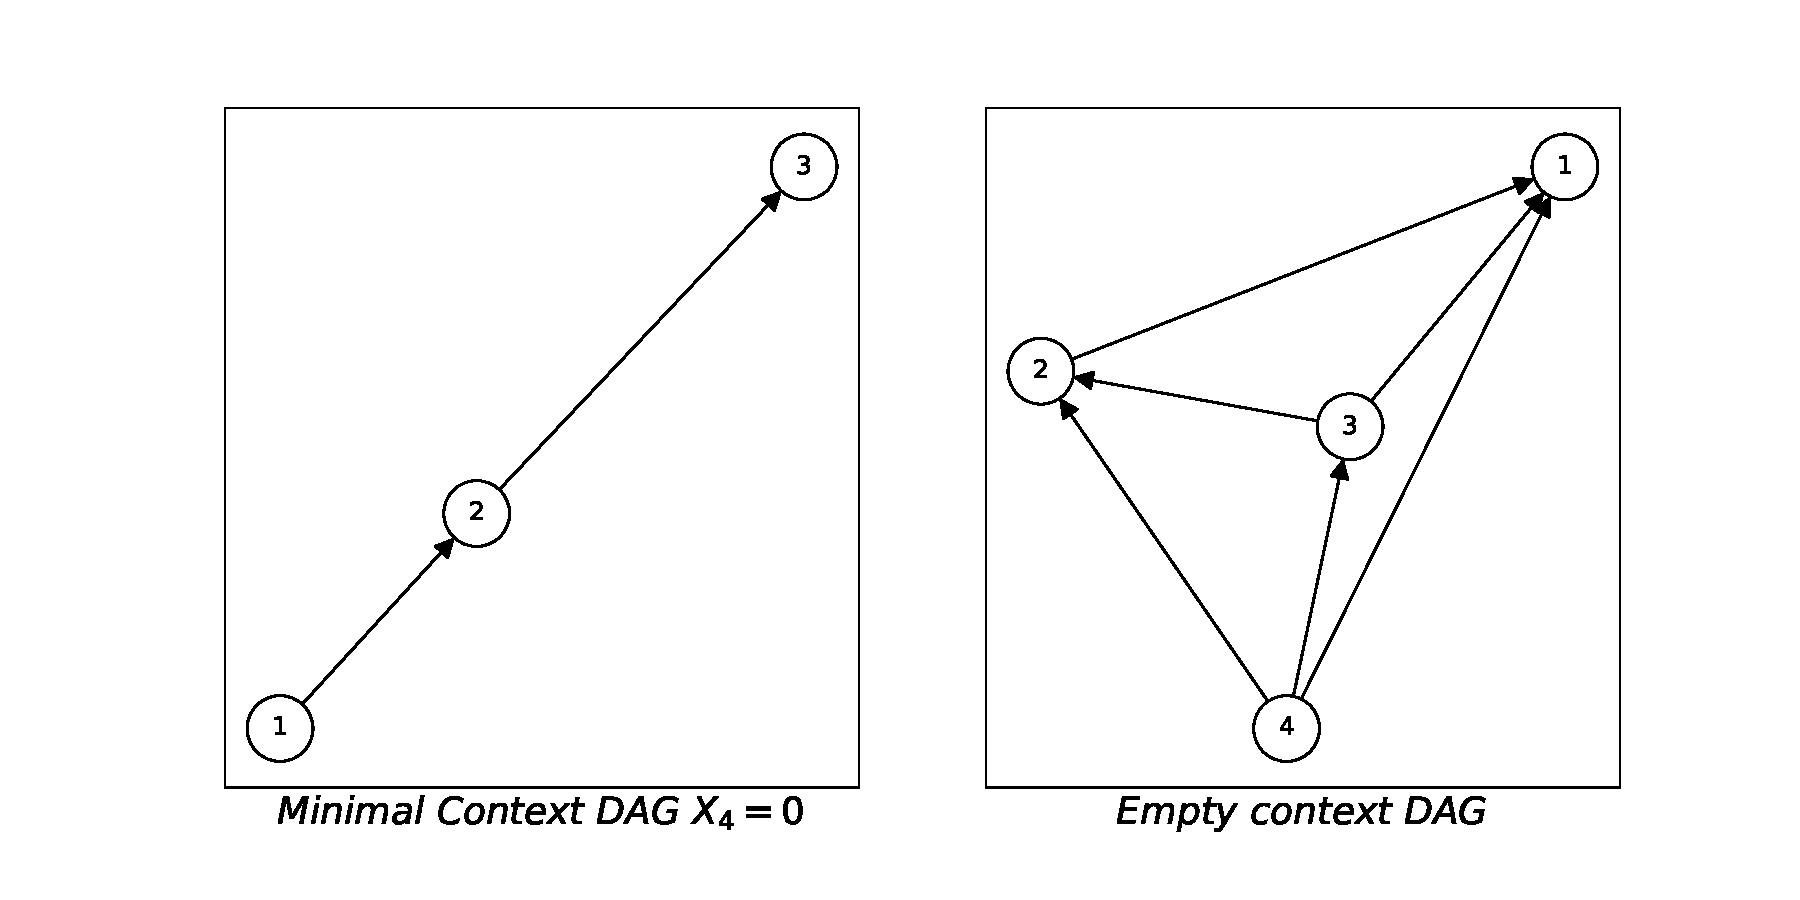
\includegraphics[width=1\linewidth]{figures/exampleonallmec.pdf}}%
\caption{Example on why to consider all topological ordering of all Markov equivalent DAGs when learning a CStree}
        
   \end{floatrow}
\end{figure}


Let \(\mathbb{P}\) be the data generating distribution and suppose it is faithful to the CStree with the context graph shown above for the context \(X_4=0\). The empty context DAG could possibly be the fully connected shown above. If we do happen to learn this exact DAG as our CPDAG from the PC algorithm step, as this DAG only has one topological ordering which is 4321, there is no way to join the stages for the empty context graph with this order to encode \((X_1 \indep X_3 \,|\,X_4=0)\), in which case we do not learn the true model.


We now present the main theorem of this paper, which is the consistency guarantee for learning CStrees when we know the true causal ordering.


\begin{theorem}\label{thm:cstreepccorrectness}
Given variables $X_1,...,X_p$, assuming that the data generating distribution $\mathbb{P}$ is faithful to some unknown CStree $\mathbb{T}$ with a known causal ordering $\pi = \pi_1 \cdots \pi_p$, Algorithm \ref{alg:learncstree} is consistent, i.e. it recovers $\mathbb{T}$ as the number of samples $n \rightarrow \infty$.
\end{theorem}


\textit{Proof:
Since $\mathbb{P}$ is faithful to $\mathbb{T}$ it entails the CSI relations encoded by minimal context DAGs $\mathbb{G}_{\mathbb{T}}$. By Theorem \ref{thm:markovtheoremcstrees}, this is equivalent to $\mathbb{P}$ factorizing according to $\mathbb{T}$. Faithfulness also implies that if two nodes are in different stages, they must have different labels, since otherwise we would have a CSI relation not entailed by $\mathbb{G}_{\mathbb{T}}$. Hence in the limit of large data, we can differentiate between different stages in $\mathbb{T}$, allowing us to recover it up to Markov equivalence.
}

\section{Model selection for CStrees}
\label{sec:orgdd068b3}
If we do not know the true causal ordering, we select the CStree (or CStrees if there is more than one) with the causal ordering corresponding to the fewest stages, which is motivated by the principle of Occams razor \cite{pearl-2009-causal} since few stages imply lower model complexity and all else being equal, the simplest model is the best model. The original authors also present the \textbf{Bayesian Information Criterion (BIC)} for CStrees alongside a proof that it is locally consistent for CStrees, meaning it can be applicable to greedy search methods for CStrees. The BIC depends on two terms, the likelihood of the data, which assesses the quality of the model to explain the observed data, and a complexity term that depends on the amount of observed data and the free parameters of the model, with the idea being that models with more parameters should be penalized. Importantly, this helps against overfitting since one can simply add more parameters to the model to maximize the likelihood.


For a general model with random variables \(X_1,...,X_p\) the likelihood of observing a sample \((x_1,...,x_p)\) can be described as below  \footnote{Here we compactify the notation further - $X_{\{1,...,p\}}=x_{\{1,...,p\}}$ is the same as $X_{\{1,...,p\}}=x_1\cdots x_p$ which is $X_1=x_1,...,X_p=x_p$.} 
.


\begin{align*}
\mathbb{P}(X_{\{1,...,p\}}=x_{\{1\cdots x_p\}}) =\mathbb{P}(X_i=x_i|X_{\{i-1,...,1\}}=x_{\{i-1,...,1 \}})\\\cdots\mathbb{P}(X_2=x_2|X_1=x_1)\mathbb{P}(X_1=x_1)
\end{align*}

In the CStree model, independence is implied from the staging of the tree, and each distribution in the product above depends on the fixed context of the node in the CStree representing that distribution. Denoting \(C_i\) to be the context variables of the context of the node \(x_{1\cdots i}\), this gives the following.

\begin{align*}
\mathbb{P}(X_{\{1,...,p\}}=x_{\{1,..., p\}}) =\prod_{i=1}^p \mathbb{P}(X_i=x_i|X_{C_i}=x_{C_i})
\end{align*}


In order to get these values from the data, we denote \(\mathbb{U}\) to be \textbf{contingency table} of the data, which a multi-dimensional array  \footnote{This is the same as tensors in the context of computer science}   with dimensions \(d_1 \times \cdots \times d_p\), where \(d_i\) is the number of possible outcomes for variable \(X_i\). Given a sample \((x_1,...,x_p)\), the value in \(\mathbb{U}[(x_1,...,x_p)]\) is the number of times we have this sample in the dataset. The marginalized contingency table \(\mathbb{U}_C\) represents the table after summing over the axes which are not in \(C\). An important case is when \(C\) is the empty set, which results in the marginal table to be 1 dimensional scalar and is the total number of samples in the dataset - when having a stage with an empty context this reflects the conditional distribution for the corresponding variable to simply be the ratio of its outcomes in the dataset. This allows the following compact representation for the likelihood \cite{duarte-2021-repres-contex} for a tree with levels \((L_1,...,L_p) \sim (X_1,...,X_p)\).

\begin{align*}
\mathbb{P}(X_{\{1,...,p\}}=x_{\{1,..., p\}}) = \prod_{k=1}^p \frac{\mathbb{U}_{C \cup k}[x_{C \cup k}]}{\mathbb{U}_{C}[x_{C}]}
\end{align*}

Given \(n\) samples arranged into a \(n \times p\) array \(\mathbb{D}\), and under the assumption that they are independent, the total likelihood is simply the product over all samples in \(\mathbb{D}\).


The free parameters is \(d=\sum_{k=1}^{p-1} (|\mathcal{X}_k| - 1)S_k\) where \(S_k\) is the number of distinct stages in level \(k\) \cite{duarte-2021-repres-contex}. The  BIC score for a CStree \(\mathbb{T}\) with observed data \(\mathbb{D}\) is then

\begin{align*}
\textbf{BIC}(\mathbb{T},\mathbb{D}) = \log\mathbb{P}(\mathbb{D}\,|\,\mathbb{T}) - \frac{d}{2}\log(n)
\end{align*}



\chapter{Experiments}
\label{sec:org4566e0b}
The aim of this section is to test the theory presented so far in both synthetic and real world data. Namely, we ask ourselves the following questions.

\begin{enumerate}
\item Given a DAG and a causal ordering, is there a difference between learning the context-specific independence relations after encoding the CI relations from the DAG into CStree, or without encoding any of these CI relations?
\item Is the CStree property assumption reasonable in practice?
\item How sensitive are the results to the method used to determine whether nodes belong to the same stage?
\item How sensitive are the results when using different DAG model learning algorithms to learn the set of possible causal orderings?
\item How well do our learnt CStrees compared to staged tree models learnt using different algorithms?
\end{enumerate}


Throughout this section we omit the final layer of nodes for all the CStrees since they always belong to the singleton stage. For minimal contexts, we compute the general minimal contexts rather than the pairwise minimal contexts. We note that for the experiments we run below, the pairwise minimal contexts and general minimal contexts are equivalent.



\section{Synthetic data}
\label{sec:orgaaa7594}
We start by generating random DAGs and generating the corresponding CStrees as per Algorithm \ref{alg:dagtocstree}. We run a sanity check by generating CStrees from DAGs in the 2 extreme cases,  the fully connected DAG and the empty DAG. The results are included in the Appendix. For random DAGs, we first choose the number of variables (nodes in the DAG) \(p\), then we choose an edge with probability \(p_{edge} \in (0,1)\), and keep the edge \((u,v)\) if and only if \(u<v\). The causal ordering is chosen as \(12\cdots p\). We show the generated CStree below, and recover the original DAG as a minimal context DAG with the empty context with Algorithm \ref{alg:mcdags}. 




\begin{figure}[!h]\label{fig:dagtocstree_cstree}
   \begin{floatrow}
\ffigbox{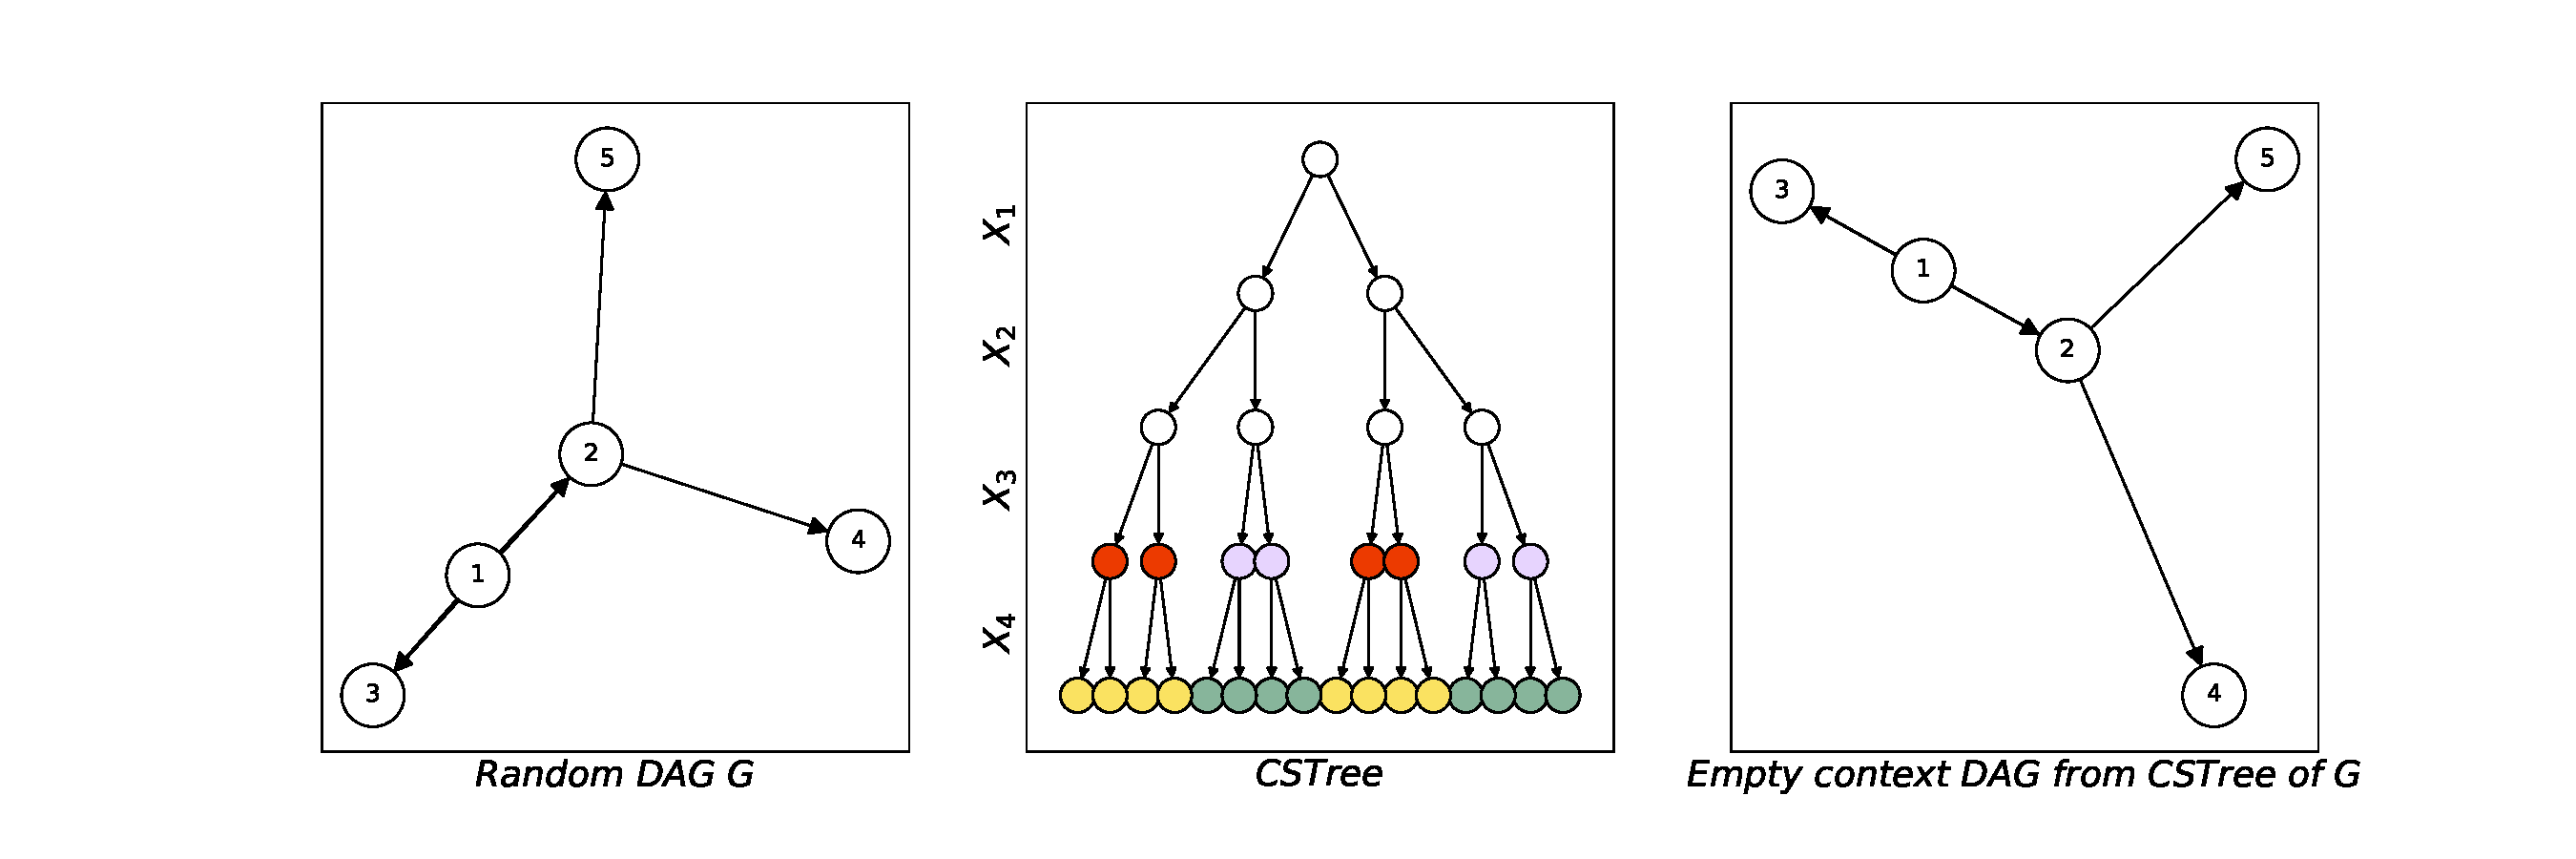
\includegraphics[width=1.1\linewidth]{figures/dagtocstreetoemptycontextdag.pdf}}%
\
\caption{Generating CStrees from random DAGs and recovering the original random DAG from the CStree with ordering 1234 using Algorithm \ref{alg:mcdags}}
        
   \end{floatrow}
\end{figure}


The following table summarizes the empirical space time complexity of generating a CStree from certain random DAGs generated from the aforementioned procedure.

\begin{table}[htbp]
\caption{Statistics from generating CStrees for random DAGs, Space refers to the amount of RAM occupied by the CStree structure, and time refers to the amount of time taken to encode the CI relations in the DAG to the CStree. We see the space complexity increase exponentially as mentioned. The time complexity however can depend on the DAG structure, however the trend suggests an exponential increase.}
\centering
\begin{tabular}{r|r|r|r}
\hline
\(p_{edge}\) & DAG Nodes & Space  (GB) & Time  (s)\\
\hline
0.2 & 20 & 1.203 & 14\\
0.2 & 21 & 2.422 & 43\\
0.2 & 22 & 4.875 & 74\\
0.2 & 23 & 9.812 & 240\\
\end{tabular}
\end{table}


Next we generate a random DAG \(\mathbb{G}\) using the procedure above, and then generate samples from this DAG, where each variable is binary valued. We then discard the DAG and apply Algorithm \ref{alg:cstreepc2} on the generated samples. For nodes which are adjacent to another node, we sample the data by constructing a conditional probability distribution table by taking the parents of the nodes, and creating one row for each possible outcome of the parents. In this binary case, if a variable \(X_i\) has \(d\) parents \(X_{PA_{\mathbb{G}}(i)}\), the corresponding table has \(2^d\) rows. The \(2\) columns represent the outcome \(0\) and \(1\) respectively. The probability values are filled by taking a row corresponding to some outcome of the parents, and assigning the probability of \(X_i=0\) under this outcome to be distributed uniformly between \([0.01,0.2]\) or \([0.8,0.99]\) each with a probability \(0.5\). The probability for \(X_i=1\) under this outcome is then simply computed such that the probabilities sum to \(1\). For the variables corresponding to nodes with no edges, we give them a Bernoulli distribution with a parameter chosen uniformly between \([0,1]\) for each such variable.



We simulate samples on 4 binary variables using the above procedure by fixing a DAG and a distribution, and sampling 2000 values from it. The random DAG we generate is shown in Figure \ref{fig:syntheticdag} We then learn the CStree using Algorithm \ref{alg:cstreepc} and recover the minimal context DAGs via Algorithm \ref{alg:mcdags} for a random subsample of 500 and all 2000 of these samples. The results of these are shown in Figure  We choose 4 variables due to limitations of applying the context-specific conditional independence axioms. We also set the ordering to be 1234.

\begin{figure}[]\label{fig:syntheticdag}
 \centering
\ffigbox{\includegraphics[width=0.5\linewidth]{figures/synthetic_dag.pdf}}%
\caption{Random DAG generated to test Algorithm \ref{alg:cstreepc} and \ref{alg:mcdags} on synthetic data. The exact probability distribution values are\\ $\mathbb{P}(X_4=0\,|\,X_{\{1,2,3\}}=000)=0.06$,\\ $\mathbb{P}(X_4=0\,|\,X_{\{1,2,3\}}=001)=0.85$,\\
$\mathbb{P}(X_4=0\,|\,X_{\{1,2,3\}}=010)=0.87$,\\ $\mathbb{P}(X_4=0\,|\,X_{\{1,2,3\}}=011)=0.1$,\\
$\mathbb{P}(X_4=0\,|\,X_{\{1,2,3\}}=100)=0.1$,\\ $\mathbb{P}(X_4=0\,|\,X_{\{1,2,3\}}=101)=0.16$,\\
$\mathbb{P}(X_4=0\,|\,X_{\{1,2,3\}}=110)=0.94$,\\
$\mathbb{P}(X_4=0\,|\,X_{\{1,2,3\}}=111)=0.86$,\\
$\mathbb{P}(X_1=0)=0.14$,$\mathbb{P}(X_2=0)=0.39$,$\mathbb{P}(X_3=0)=0.37$}

\end{figure}


\begin{figure}[!h]\label{fig:mc_dags500}
   \begin{floatrow}
\ffigbox{\includegraphics[width=1.1\linewidth]{figures/mcdags_5002.pdf}}%
 \caption{CSTree and corresponding minimal context DAGs from the 500 samples from the synthetic DAG experiment.}
        
   \end{floatrow}
\end{figure}


\begin{figure}[!h]\label{fig:mc_dags2000}
   \begin{floatrow}
\ffigbox{\includegraphics[width=1.1\linewidth]{figures/mcdags_2000.pdf}}%
 \caption{CSTree and corresponding minimal context DAG from the 2000 samples from the synthetic DAG experiment.}
        
   \end{floatrow}
\end{figure}


We expect that in the limit of large data, the CSI relations we learn would converge to the CI relations implied by the DAG. The above procedure could produce non empty minimal contexts for several reasons, for example due to small sample sizes, or errors in the context-specific independence testing procedure. Here we use the Epps-Singleton test \cite{epps-1986-omnib-test}. We see that the empty context DAG does not correspond to the true DAG in this case. Although this did not happen significantly often on our synthetic data experiments, in practice the CI testing used to learn the DAG model and the CSI relations can be highly unstable, and this will be a common theme in this chapter. For example it is possible for the CI testing to erroneously encode a CI relation, implying that that the independence relation holds for all outcomes whilst in reality it only holds under specific contexts. Similarly, it is possible for the CSI tests to erroneously merge stages, entailing a CSI relation that does not exist. 


In order to assess the influence of the CI relations from the DAG in the final CStree, we tested the use of Algorithm \ref{alg:cstreepc} on the same 2000 samples used to get the results in \ref{fig:mc_dags2000}. The results are shown in Figure \ref{fig:mcdags_csi}. In this case we do recover the true DAG. Since this CStree was learnt only using the CSI relations, it is reasonable to assume that the errors in CI testing contributed to the previous result. This suggests that we could expect better performance if we only use DAG discovery algorithms, such as the PC algorithm, to learn possible orderings of the true CStree rather than to learn an approximation of the CStree model itself through the CI relations encoded in them.

\begin{figure}[!h]\label{fig:mcdags_csi}
   \begin{floatrow}
\ffigbox{\includegraphics[width=1.1\linewidth]{figures/mcdags_csi.pdf}}%
 \caption{CSTree and corresponding minimal context DAG from the same samples as in Figure \ref{fig:mc_dags2000} but without encoding the CI relations from the initial DAG.}
        
   \end{floatrow}
\end{figure}

 \newpage 
\section{Coronary disease data}
\label{sec:org4a3b5a2}

This is a dataset consisting of features which might increase the risk for coronary thrombosis, and consists of 1841 samples from men \cite{reinis-1981-progn-signif}.  These features are detailed below.
\begin{center}
\begin{tabular}{l|r|l}
\hline
Variable name & Node & Outcomes\\
\hline
Smoking & 1 & \(\{ Yes,No \}\)\\
Strenuous mental work & 2 & \(\{ Yes,No \}\)\\
Strenuous physical work & 3 & \(\{ Yes,No \}\)\\
Systolic blood pressure & 4 & \(\{(-\infty,140],(140,\infty)\}\)\\
Ratio of beta and alpha lipoproteins & 5 & \(\{(-\infty,3],(3,\infty)\}\)\\
Coronary heart disease family history & 6 & \(\{ Yes,No \}\)\\
\end{tabular}
\end{center}


This data set does not require further pre-processing since the outcome space is already categorical, and there were no missing values.


We first perform the following experiment: Learn a DAG model from both the PC algorithm and the Hill climbing search algorithm \cite{koller-2009-probab,ankan-2015} . Now for each topological ordering of all the DAGs which are Markov equivalent, we store the following CStrees:
\begin{enumerate}
\item The CStree generated from the DAG itself, from Algorithm \ref{alg:dagtocstree}.
\item The CStree learnt only from context-specific information without encoding the CI relations from the DAG, from Algorithm \ref{alg:cstreepc}.
\item The CStree learnt from encoding the CI relations from the DAG and then learning further context-specific information, from Algorithm \ref{alg:cstreepc2}.
\end{enumerate}

For each of the cases above we create/merge stages using the Anderson-Darling test \cite{scholz-1987-k-sampl}, the Epps-Singleton test \cite{epps-1986-omnib-test}, and the symmetric KL divergence  \footnote{Also called the Kullback-Leibler divergence}  with different threshold values. The use of the symmetric KL divergence is motivated by the unreliability of conditional independence testing in practice \cite{shah-2020-hardn-condit}. Given 2 distributions \(\mathbb{P}, \mathbb{Q}\) over the same discrete state space \(\mathcal{X}\), the symmetric KL divergence is as follows. 



\begin{align*}
D_{SKL}(\mathbb{P} \, , \, \mathbb{Q}) = \sum_{x \in \mathcal{X}} \mathbb{P}(X=x)\log \frac{\mathbb{P}(X = x)}{\mathbb{Q}(X=x)} + \mathbb{Q}(X=x)\log \frac{\mathbb{Q}(X = x)}{\mathbb{P}(X=x)}.
\end{align*}

The symmetric KL (SKL) divergence can be thought of as a value that quantifies the distance between the distributions \(\mathbb{P}\) and \(\mathbb{Q}\). Notably, it returns \(0\) if \(\mathbb{P}=\mathbb{Q}\) for all outcomes \(x \in \mathcal{X}\).


The output of the PC algorithm is a CPDAG, and whilst the outcome of the Hill climbing algorithm is a DAG, there are computationally efficient algorithms that allow us to generate the CPDAG that represents its MEC \cite{chickering-2002-learn-equiv}. Once we have the CPDAG, generating the DAGs consistent with it involves orienting the undirected edges such that we do not form any new v-structures and do not create cycles. 


We apply Algorithms \ref{alg:dagtocstree}, \ref{alg:cstreepc}, and \ref{alg:cstreepc2} to the setup above, and record the CStrees with the minimum number of stages over all possible causal orderings, alongside their BIC scores. Note that it is possible for multiple non-statistically (non-Markov) equivalent CStrees to have stages equal to the minimum number of stages. This can occur, for example when the underlying true causal structure is not faithful to a CStree but is instead faithful to a non-CStree staged tree. It can also occur due to testing errors induced by small sample size. In this case, we select the BIC-optimal CStree since the BIC is a score-equivalent and consistent estimator for CStrees \cite{duarte-2021-repres-contex}. The score-equivalence property implies in the limit of large data, all statistically equivalent equivalent CStrees will have the same BIC score. We call this \textbf{experimental setup 1}, and the results of this experiment for the coronary dataset are summarized in the Table \ref{table:coronary1}.





% Please add the following required packages to your document preamble:
% \usepackage{multirow}
\begin{table*}[]\label{table:coronary1}
\begin{tabular}{cccccccccccccccc}
\cline{3-12}
                        & \multicolumn{1}{c|}{\multirow{\begin{tabular}[c]{@{}c@{}}Goal:\\ Min stages\end{tabular}}} & \multicolumn{2}{c|}{Anderson}                                  & \multicolumn{2}{c|}{Epps}                                  & \multicolumn{2}{c|}{SKL $5 \times 10^{-5}$}                            & \multicolumn{2}{c|}{SKL $5 \times 10^{-6}$}                            & \multicolumn{2}{c|}{SKL $5 \times 10^{-7}$}                                     &  &  &  &  \\ \cline{3-12}
                        & \multicolumn{1}{c|}{}                                                                            & \multicolumn{1}{c|}{Stages}     & \multicolumn{1}{c|}{BIC}     & \multicolumn{1}{c|}{Stages} & \multicolumn{1}{c|}{BIC}     & \multicolumn{1}{c|}{Stages} & \multicolumn{1}{c|}{BIC}     & \multicolumn{1}{c|}{Stages} & \multicolumn{1}{c|}{BIC}     & \multicolumn{1}{c|}{Stages} & \multicolumn{1}{c|}{BIC}              &  &  &  &  \\ \cline{3-12}
                        &                                                                                                  &                                 &                              &                             &                              &                             &                              &                             &                              &                             &                                       &  &  &  &  \\ \cline{2-12}
\multicolumn{1}{c|}{}   & \multicolumn{1}{c|}{DAG}                                                                         & \multicolumn{1}{c|}{18}         & \multicolumn{1}{c|}{-6739.4} & \multicolumn{1}{c|}{18}     & \multicolumn{1}{c|}{-6739.4} & \multicolumn{1}{c|}{18}     & \multicolumn{1}{c|}{-6739.4} & \multicolumn{1}{c|}{18}     & \multicolumn{1}{c|}{-6739.4} & \multicolumn{1}{c|}{18}     & \multicolumn{1}{c|}{-6739.4}          &  &  &  &  \\ \cline{2-12}
\multicolumn{1}{c|}{\rotatebox{90}{PC}} & \multicolumn{1}{c|}{\begin{tabular}[c]{@{}c@{}}CSTree \\ w/o DAG\end{tabular}}                     & \multicolumn{1}{c|}{\textbf{6}} & \multicolumn{1}{c|}{-6793.7} & \multicolumn{1}{c|}{13}     & \multicolumn{1}{c|}{-6812.1} & \multicolumn{1}{c|}{23}     & \multicolumn{1}{c|}{-6757.1} & \multicolumn{1}{c|}{31}     & \multicolumn{1}{c|}{-7032.3} & \multicolumn{1}{c|}{44}     & \multicolumn{1}{c|}{-6753.4}          &  &  &  &  \\ \cline{2-12}
\multicolumn{1}{c|}{}   & \multicolumn{1}{c|}{\begin{tabular}[c]{@{}c@{}}CSTree \\ with DAG\end{tabular}}                   & \multicolumn{1}{c|}{8}          & \multicolumn{1}{c|}{-6771.3} & \multicolumn{1}{c|}{11}     & \multicolumn{1}{c|}{-6780.4} & \multicolumn{1}{c|}{15}     & \multicolumn{1}{c|}{-6775.4} & \multicolumn{1}{c|}{18}     & \multicolumn{1}{c|}{-6739.4} & \multicolumn{1}{c|}{18}     & \multicolumn{1}{c|}{-6739.4}          &  &  &  &  \\ \cline{2-12}
                        &                                                                                                  &                                 &                              &                             &                              &                             &                              &                             &                              &                             &                                       &  &  &  &  \\ \cline{2-12}
\multicolumn{1}{c|}{}   & \multicolumn{1}{c|}{DAG}                                                                         & \multicolumn{1}{c|}{28}         & \multicolumn{1}{c|}{-6714.78} & \multicolumn{1}{c|}{28}     & \multicolumn{1}{c|}{-6714.8} & \multicolumn{1}{c|}{28}     & \multicolumn{1}{c|}{-6714.8} & \multicolumn{1}{c|}{28}     & \multicolumn{1}{c|}{-6714.8} & \multicolumn{1}{c|}{28}     & \multicolumn{1}{c|}{-6714.8}          &  &  &  &  \\ \cline{2-12}
\multicolumn{1}{c|}{\rotatebox{90}{HC}} & \multicolumn{1}{c|}{\begin{tabular}[c]{@{}c@{}}CSTree \\ w/o DAG\end{tabular}}                     & \multicolumn{1}{c|}{7}          & \multicolumn{1}{c|}{-6791.0} & \multicolumn{1}{c|}{30}     & \multicolumn{1}{c|}{-6841.9} & \multicolumn{1}{c|}{24}     & \multicolumn{1}{c|}{-6802.9} & \multicolumn{1}{c|}{36}     & \multicolumn{1}{c|}{-6828.1} & \multicolumn{1}{c|}{47}     & \multicolumn{1}{c|}{-6755.9}          &  &  &  &  \\ \cline{2-12}
\multicolumn{1}{c|}{}   & \multicolumn{1}{c|}{\begin{tabular}[c]{@{}c@{}}CSTree \\ with DAG\end{tabular}}                   & \multicolumn{1}{c|}{8}          & \multicolumn{1}{c|}{-6788.7} & \multicolumn{1}{c|}{15}     & \multicolumn{1}{c|}{-6809.7} & \multicolumn{1}{c|}{21}     & \multicolumn{1}{c|}{-6794.9} & \multicolumn{1}{c|}{20}     & \multicolumn{1}{c|}{-6786.9} & \multicolumn{1}{c|}{27}     & \multicolumn{1}{c|}{\textbf{-6711.0}} &  &  &  &  \\ \cline{2-12}
                        &                                                                                                  &                                 &                              &                             &                              &                             &                              &                             &                              &                             &                                       &  &  &  &  \\
                        &                                                                                                  &                                 &                              &                             &                              &                             &                              &                             &                              &                             &                                       &  &  &  &  \\
                        &                                                                                                  &                                 &                              &                             &                              &                             &                              &                             &                              &                             &                                       &  &  &  &  \\
                        &                                                                                                  &                                 &                              &                             &                              &                             &                              &                             &                              &                             &                                       &  &  &  &  \\
                        &                                                                                                  &                                 &                              &                             &                              &                             &                              &                             &                              &                             &                                       &  &  &  &  \\
                        &                                                                                                  &                                 &                              &                             &                              &                             &                              &                             &                              &                             &                                       &  &  &  & 

\caption{Experimental setup 1 on the coronary dataset. Each cell under the column "Stages" is the minimum number of stages amongst all causal orderings generated from the either the PC or Hill Climbing algorithm, for different staging criteria. Many orderings produce CStrees with the same number of stages, in which case the BIC score in the table above is the maximum over those CStrees.}
\end{tabular}
\end{table*}

The CPDAG from the PC algorithm gave 12 orderings, whilst the Hill climbing algorithm provided 16, where we optimized for the BIC score.


Here we see that the minimum number of stages over all the configurations is 6, which results in the CStree shown in Figure \ref{fig:coronary1}. The causal ordering is 346125, and we get this CStree by learning the original DAG using the PC algorithm, followed by the Anderson-Darling test to learn context-specific information without encoding the CI relations from the original DAG. However it can be seen that the BIC score is lower compared to the CStree generated from the DAG itself and the CStree learnt using the CI relations in the DAG before learning the context-specific information. The latter CStree also has more stages than the CStree learnt without using the CI relations, which can be explained by the possibility that the CI relation(s) encoded in the DAG may have put nodes in the same stage, which otherwise may have been merged from the context-specific testing procedure. These observations collectively imply that, possibly due to the small sample size, or violation of the CStree faithfulness assumption, the minimum stage condition for selecting the best CStree is not reasonable. Instead, we can take the BIC-optimal CStree with the fewest stages learned over all the configurations, as this provides a balance between the model fit and sparsity.

\begin{figure}[]\label{fig:coronary1}
   \begin{floatrow}
\ffigbox{\includegraphics[width=1.1\linewidth]{figures/coronary_minstages.pdf}}%
\caption{CStree for the coronary dataset with the lowest number of stages, which has ordering 346125 and corresponds to a DAG model.}
        
   \end{floatrow}
\end{figure}

We note that we do learn a CStree with 8 stages which is not a DAG model, corresponding to the ordering 431265, which we show below in Figure \ref{fig:coronary_minstages_nodag}.


\begin{figure}[]\label{fig:coronary_minstages_nodag}
   \begin{floatrow}
\ffigbox{\includegraphics[width=1.1\linewidth]{figures/coronary_minstages_nondag3.pdf}}%
\caption{CStree with causal ordering 431265 learnt from the coronary dataset which has 8 stages and does not correspond to a DAG model.}
        
   \end{floatrow}
\end{figure}

Among the trees with the fewest stages, whose information is shown in Table \ref{table:coronary1}, the CStree with the highest BIC score we recorded is generated with the ordering 541326, using the symmetric KL divergence with a threshold of \(5\times 10^{-7}\) for the staging procedure, from the DAG learnt from the Hill Climbing algorithm and without encoding the CI relations from it. It shown in Figure \ref{fig:coronary2}. We see that this CStree has 30 stages, which motivates us to define the \textbf{experimental setup 2}, where we find the CStree with the highest BIC score instead of the minimum number of stages as in experimental setup 1. We show the results of this in Table \ref{table:coronary2}.



\begin{figure}[]\label{fig:coronary2}
   \begin{floatrow}
\ffigbox{\includegraphics[width=1.1\linewidth]{figures/coronary_maxbic.pdf}}%
\caption{CStree with the highest BIC score among all CStrees with the minimum number of stages in experimental setup 1 for the coronary dataset, which has ordering 541326.}
        
   \end{floatrow}
\end{figure}



% Please add the following required packages to your document preamble:
% \usepackage{multirow}
\begin{table*}[]\label{table:coronary2}
\begin{tabular}{cccccccccccccccc}
\cline{3-12}
                        & \multicolumn{1}{c|}{\multirow{\begin{tabular}[c]{@{}c@{}}Goal:\\ Max BIC\end{tabular}}} & \multicolumn{2}{c|}{Anderson}                                  & \multicolumn{2}{c|}{Epps}                                  & \multicolumn{2}{c|}{SKL $5 \times 10^{-5}$}                            & \multicolumn{2}{c|}{SKL $5 \times 10^{-6}$}                            & \multicolumn{2}{c|}{SKL $5 \times 10^{-7}$}                                     &  &  &  &  \\ \cline{3-12}
                        & \multicolumn{1}{c|}{}                                                                            & \multicolumn{1}{c|}{Stages}     & \multicolumn{1}{c|}{BIC}     & \multicolumn{1}{c|}{Stages} & \multicolumn{1}{c|}{BIC}     & \multicolumn{1}{c|}{Stages} & \multicolumn{1}{c|}{BIC}     & \multicolumn{1}{c|}{Stages} & \multicolumn{1}{c|}{BIC}     & \multicolumn{1}{c|}{Stages} & \multicolumn{1}{c|}{BIC}              &  &  &  &  \\ \cline{3-12}
                        &                                                                                                  &                                 &                              &                             &                              &                             &                              &                             &                              &                             &                                       &  &  &  &  \\ \cline{2-12}
\multicolumn{1}{c|}{}   & \multicolumn{1}{c|}{DAG}                                                                         & \multicolumn{1}{c|}{18}         & \multicolumn{1}{c|}{-6739.4} & \multicolumn{1}{c|}{18}     & \multicolumn{1}{c|}{-6739.4} & \multicolumn{1}{c|}{18}     & \multicolumn{1}{c|}{-6739.4} & \multicolumn{1}{c|}{18}     & \multicolumn{1}{c|}{-6739.4} & \multicolumn{1}{c|}{18}     & \multicolumn{1}{c|}{-6739.4}          &  &  &  &  \\ \cline{2-12}
\multicolumn{1}{c|}{\rotatebox{90}{PC}} & \multicolumn{1}{c|}{\begin{tabular}[c]{@{}c@{}}CSTree \\ w/o DAG\end{tabular}}                     & \multicolumn{1}{c|}{\textbf{7}} & \multicolumn{1}{c|}{-6783.7} & \multicolumn{1}{c|}{13}     & \multicolumn{1}{c|}{-6812.1} & \multicolumn{1}{c|}{23}     & \multicolumn{1}{c|}{-6757.1} & \multicolumn{1}{c|}{43}     & \multicolumn{1}{c|}{-6749.6} & \multicolumn{1}{c|}{44}     & \multicolumn{1}{c|}{-6753.4}          &  &  &  &  \\ \cline{2-12}
\multicolumn{1}{c|}{}   & \multicolumn{1}{c|}{\begin{tabular}[c]{@{}c@{}}CSTree \\ with DAG\end{tabular}}                   & \multicolumn{1}{c|}{8}          & \multicolumn{1}{c|}{-6771.3} & \multicolumn{1}{c|}{11}     & \multicolumn{1}{c|}{-6780.4} & \multicolumn{1}{c|}{15}     & \multicolumn{1}{c|}{-6775.4} & \multicolumn{1}{c|}{18}     & \multicolumn{1}{c|}{-6739.4} & \multicolumn{1}{c|}{18}     & \multicolumn{1}{c|}{-6739.4}          &  &  &  &  \\ \cline{2-12}
                        &                                                                                                  &                                 &                              &                             &                              &                             &                              &                             &                              &                             &                                       &  &  &  &  \\ \cline{2-12}
\multicolumn{1}{c|}{}   & \multicolumn{1}{c|}{DAG}                                                                         & \multicolumn{1}{c|}{31}         & \multicolumn{1}{c|}{-6714.8} & \multicolumn{1}{c|}{28}     & \multicolumn{1}{c|}{-6714.8} & \multicolumn{1}{c|}{28}     & \multicolumn{1}{c|}{-6714.8} & \multicolumn{1}{c|}{28}     & \multicolumn{1}{c|}{-6714.8} & \multicolumn{1}{c|}{28}     & \multicolumn{1}{c|}{-6714.8}          &  &  &  &  \\ \cline{2-12}
\multicolumn{1}{c|}{\rotatebox{90}{HC}} & \multicolumn{1}{c|}{\begin{tabular}[c]{@{}c@{}}CSTree \\ w/o DAG\end{tabular}}                     & \multicolumn{1}{c|}{8}          & \multicolumn{1}{c|}{-6775.5} & \multicolumn{1}{c|}{31}     & \multicolumn{1}{c|}{-6826.4} & \multicolumn{1}{c|}{27}     & \multicolumn{1}{c|}{-6802.8} & \multicolumn{1}{c|}{39}     & \multicolumn{1}{c|}{-6828.0} & \multicolumn{1}{c|}{47}     & \multicolumn{1}{c|}{-6755.9}          &  &  &  &  \\ \cline{2-12}
\multicolumn{1}{c|}{}   & \multicolumn{1}{c|}{\begin{tabular}[c]{@{}c@{}}CSTree \\ with DAG\end{tabular}}                   & \multicolumn{1}{c|}{9}          & \multicolumn{1}{c|}{-6773.2} & \multicolumn{1}{c|}{16}     & \multicolumn{1}{c|}{-6794.1} & \multicolumn{1}{c|}{24}     & \multicolumn{1}{c|}{-6786.6} & \multicolumn{1}{c|}{20}     & \multicolumn{1}{c|}{-6786.49} & \multicolumn{1}{c|}{27}     & \multicolumn{1}{c|}{\textbf{-6711.0}} &  &  &  &  \\ \cline{2-12}
                        &                                                                                                  &                                 &                              &                             &                              &                             &                              &                             &                              &                             &                                       &  &  &  &  \\
                        &                                                                                                  &                                 &                              &                             &                              &                             &                              &                             &                              &                             &                                       &  &  &  &  \\
                        &                                                                                                  &                                 &                              &                             &                              &                             &                              &                             &                              &                             &                                       &  &  &  &  \\
                        &                                                                                                  &                                 &                              &                             &                              &                             &                              &                             &                              &                             &                                       &  &  &  &  \\
                        &                                                                                                  &                                 &                              &                             &                              &                             &                              &                             &                              &                             &                                       &  &  &  &  \\
                        &                                                                                                  &                                 &                              &                             &                              &                             &                              &                             &                              &                             &                                       &  &  &  & 

\caption{Experimental setup 2 on the coronary dataset, the only difference to experimental setup 1 is that we now maximize the BIC score over all possible causal orderings.}
			\end{tabular}
\end{table*}


The results of Table \ref{table:coronary1} and \ref{table:coronary2} show that the BIC-optimal CStree configuration still remains the same. In general, the differences between experimental setup 1 and 2 on this dataset show that we can find CStrees with a higher BIC score given the same configuration i.e. merging procedure and initial DAG learning algorithm, at the cost of more stages.




In order to compare our CStrees with similar staged trees, we run another experiment. First take the BIC optimal CStree that we have learnt which does not correspond to a DAG model. Take the ordering of this tree, and then fit corresponding staged trees using score-based learning algorithms, optimizing the BIC score \cite{carli-2020-r-packag}. The algorithms used to fit the staged trees are the following \cite{collazo-2018-chain}:


\begin{enumerate}
\item Hill climbing - Start from the full independence model, then in a greedy manner, for each node, either assign it an existing stage or create a new stage depending on whichever option best increases the score.
\item Backward hill climbing - Similar to hill climbing except we start from a full model, i.e. one where each node belongs to a singleton stage.
\item Backward joining - Start from the full model, and iteratively merge stages depending on whether a certain measure between them is below a threshold. We use the KL divergence with twice the threshold which gave us the BIC optimal CStree from our methods.
\item Hierarchical clustering - Start from a full model, and iteratively cluster nodes in level \(k\) to \(c_k\) clusters using hierarchical clustering. We use the total variation measure alongside 2 clusters for each level.
\end{enumerate}



We call our approach to fit the CStree modified Algorithm \ref{alg:cstreepc}/\ref{alg:cstreepc2} since the BIC optimal CStree is not necessarily learnt using the PC algorithm to get the initial DAG.

We call this \textbf{experimental setup 3}, and detail the results of it on the coronary dataset below in Table \ref{tab:org9f423fa}. None of the staged trees learnt by algorithms (1)-(4) above are CStrees, and they are included in the Appendix.

\begin{table}[htbp]
\caption{\label{tab:org9f423fa}Experimental setup 3 on the coronary dataset}
\centering
\begin{tabular}{l|l|r|r}
\hline
Model & Algorithm & BIC & Stages\\
\hline
CStree & Modified Algorithm \ref{alg:cstreepc} /\ref{alg:cstreepc2} & -6729.5 & 30\\
Non-CStree & Hill climbing & -6645.3 & 11\\
Non-CStree & Backward hill climbing & -6641.1 & 13\\
Non-CStree & Backward joining & -6790.4 & 57\\
Non-CStree & Hierarchical clustering & -6654.7 & 10\\
\end{tabular}
\end{table}



We see that the staged trees achieve a higher BIC score, which is probably due to their greater flexibility.


In order to generate the sequence of DAGs that capture the context-specific causal information from this dataset, we remove one variable for computational feasibility. We remove the variable that results in the highest BIC score after its removal, which in this case is the variable corresponding to systolic blood pressure (variable 4). The initial DAG is generated from the PC algorithm, and we learn the tree structure using both the CI relations from the DAG and the context-specific staging procedure using the symmetric KL divergence with a threshold of \(5\times 10^{-5}\). We choose the BIC optimal tree rather the one with the fewest stages, since the latter results in a context-specific closure which could be computed in a reasonable amount of time.  This results in the CStree with ordering 62351 which has \(10\) stages, shown in Figure \ref{fig:coronary_wout4}. 


\begin{figure}[!h]\label{fig:coronary_wout4}
   \begin{floatrow}
\ffigbox{\includegraphics[width=1.1\linewidth]{figures/coronary_wout4_maxbic1.pdf}}%
\caption{BIC-optimal CStree alongside the minimal context DAGs on the coronary dataset, which has the ordering 62351. The initial DAG is learnt with the PC algorithm, and the stages were merged using the symmetric KL divergence with a threshold of $5\times 10^{-5}$. }
        
   \end{floatrow}
\end{figure}


We note that in some cases one can read off the minimal contexts straight from the CStrees. One example is the CStree in Figure \ref{fig:coronary2}, where we can see that the minimal contexts are the empty context and \((X_5=1,X_4=0,X_3=1)\), where one can draw the minimal I-MAPs for the whole tree and the one for just this context through inspecting the CStree. Thus in some cases, despite the computational limitations of finding the minimal contexts automatically, we still see that we can use CStrees to more easily read context-specific causal information. In particular, it is much easier to interpret the minimal context DAGs in Figure \ref{fig:coronary_wout4} than its corresponding CStree which we learnt from observed data.

\section{Mice protein expression data}
\label{sec:orgd021f94}
This is a dataset with expression levels of 77 proteins, measured in the cerebral cortex of 8 classes of mice \cite{higuera-2015-self-organ}. There are 38 control mice and 34 trisomic mice, and for each of them 15 separate measurements were taken which gives a total of 1080 samples. The aim is to identify features that can discriminate between the 8 classes that make up all possible combinations of the following 3 binary features - Control or Trisomy, stimulated to learn or not, injected with saline or memantine. This dataset had missing values, which we handle by first inspecting the missing value counts for each feature and then removing features which had 180 or more missing values. This removes the expression data corresponding to the columns \(BAD_N, BCL2_N, H3AcK18_N, EGR1_N, H3MeK4_N\). This still leaves 72 features, which we further reduce by recursive feature elimination \cite{guyon-2002} where we first train a linear support vector classifier on all the features and prune the least important features in a greedy manner until we arrive at the number of features we want. After this we compute the medians for each feature and assign each feature to take binary outcomes depending on whether or not the value is above or below the median.



We choose 7 features and the response variable, giving a system of 8 variables. This number is chosen since this gives a maximum of 196 causal orderings which is computationally feasible, meanwhile increasing the variables to 9 and 10 increase this to 1008 and 13608 respectively if we use the PC algorithm for the initial DAG. The chosen variables are detailed below.

\begin{center}
\begin{tabular}{l|r|l}
\hline
Variable name & Node & Outcomes\\
\hline
\(AKT_N\) & 1 & \(\{(-\infty, Q^1_2],(Q^1_2, \infty) \}\)\\
\(APP_N\) & 2 & \(\{(-\infty, Q^2_2],(Q^2_2, \infty) \}\)\\
\(SOD1_N\) & 3 & \(\{(-\infty, Q^3_2],(Q^3_2, \infty) \}\)\\
\(NR2B_N\) & 4 & \(\{(-\infty, Q^4_2],(Q^4_2, \infty) \}\)\\
\(pNUMB_N\) & 5 & \(\{(-\infty, Q^5_2],(Q^5_2, \infty) \}\)\\
\(IL1B_N\) & 6 & \(\{(-\infty, Q^6_2],(Q^6_2, \infty) \}\)\\
\(SYP_N\) & 7 & \(\{(-\infty, Q^7_2],(Q^7_2, \infty) \}\)\\
Class & 8 & \(\{C_i \}_{i=1}^8\)\\
\end{tabular}
\end{center}


Here, \(Q^i_2\) refers to the median of the variable corresponding to node \(i\).

We show results of applying experimental setup 1 on this dataset in Table \ref{table:mice1} below. The PC algorithm resulted in 196 possible causal orderings, whilst the Hill climbing algorithm resulted in 12. We use the K2 score \cite{carvalho-2009-scorin-bayes} for the Hill climbing since otherwise the number of possible orderings increases to 6408.

% Please add the following required packages to your document preamble:
% \usepackage{multirow}
\begin{table*}[]\label{table:mice1}
\begin{tabular}{cccccccccccccccc}
\cline{3-12}
                        & \multicolumn{1}{c|}{\multirow{\begin{tabular}[c]{@{}c@{}}Goal:\\ Min Stages\end{tabular}}} & \multicolumn{2}{c|}{Anderson}                                  & \multicolumn{2}{c|}{Epps}                                  & \multicolumn{2}{c|}{SKL $5 \times 10^{-4}$}                            & \multicolumn{2}{c|}{SKL $5 \times 10^{-5}$}                            & \multicolumn{2}{c|}{SKL $5 \times 10^{-6}$}                            &  &  &  &  \\ \cline{3-12}
                        & \multicolumn{1}{c|}{}                                                                            & \multicolumn{1}{c|}{Stages}     & \multicolumn{1}{c|}{BIC}     & \multicolumn{1}{c|}{Stages} & \multicolumn{1}{c|}{BIC}     & \multicolumn{1}{c|}{Stages} & \multicolumn{1}{c|}{BIC}     & \multicolumn{1}{c|}{Stages} & \multicolumn{1}{c|}{BIC}     & \multicolumn{1}{c|}{Stages} & \multicolumn{1}{c|}{BIC}     &  &  &  &  \\ \cline{3-12}
                        &                                                                                                  &                                 &                              &                             &                              &                             &                              &                             &                              &                             &                              &  &  &  &  \\ \cline{2-12}
\multicolumn{1}{c|}{}   & \multicolumn{1}{c|}{DAG}                                                                         & \multicolumn{1}{c|}{154}        & \multicolumn{1}{c|}{\textbf{-5615.9}} & \multicolumn{1}{c|}{154}    & \multicolumn{1}{c|}{\textbf{-5615.9}} & \multicolumn{1}{c|}{154}    & \multicolumn{1}{c|}{\textbf{-5615.9}} & \multicolumn{1}{c|}{154}    & \multicolumn{1}{c|}{\textbf{-5615.9}} & \multicolumn{1}{c|}{154}    & \multicolumn{1}{c|}{\textbf{-5615.9}} &  &  &  &  \\ \cline{2-12}
\multicolumn{1}{c|}{\rotatebox{90}{PC}} & \multicolumn{1}{c|}{\begin{tabular}[c]{@{}c@{}}CStree \\ w/o DAG\end{tabular}}                     & \multicolumn{1}{c|}{\textbf{7}} & \multicolumn{1}{c|}{-6753.0} & \multicolumn{1}{c|}{8}      & \multicolumn{1}{c|}{-6572.7} & \multicolumn{1}{c|}{61}     & \multicolumn{1}{c|}{-5917.8} & \multicolumn{1}{c|}{64}     & \multicolumn{1}{c|}{-5823.9} & \multicolumn{1}{c|}{78}     & \multicolumn{1}{c|}{-5807.6} &  &  &  &  \\ \cline{2-12}
\multicolumn{1}{c|}{}   & \multicolumn{1}{c|}{\begin{tabular}[c]{@{}c@{}}CStree \\ with DAG\end{tabular}}                   & \multicolumn{1}{c|}{11}         & \multicolumn{1}{c|}{-6591.4} & \multicolumn{1}{c|}{11}     & \multicolumn{1}{c|}{-6591.4} & \multicolumn{1}{c|}{67}     & \multicolumn{1}{c|}{-5702.0} & \multicolumn{1}{c|}{68}     & \multicolumn{1}{c|}{-5705.4} & \multicolumn{1}{c|}{71}     & \multicolumn{1}{c|}{-5692.2} &  &  &  &  \\ \cline{2-12}
                        &                                                                                                  &                                 &                              &                             &                              &                             &                              &                             &                              &                             &                              &  &  &  &  \\ \cline{2-12}
\multicolumn{1}{c|}{}   & \multicolumn{1}{c|}{DAG}                                                                         & \multicolumn{1}{c|}{502}        & \multicolumn{1}{c|}{-6472.1} & \multicolumn{1}{c|}{502}    & \multicolumn{1}{c|}{-6472.1} & \multicolumn{1}{c|}{502}    & \multicolumn{1}{c|}{-6472.1} & \multicolumn{1}{c|}{502}    & \multicolumn{1}{c|}{-6472.1} & \multicolumn{1}{c|}{502}    & \multicolumn{1}{c|}{-6472.1} &  &  &  &  \\ \cline{2-12}
\multicolumn{1}{c|}{\rotatebox{90}{HC}} & \multicolumn{1}{c|}{\begin{tabular}[c]{@{}c@{}}CStree \\ w/o DAG\end{tabular}}                     & \multicolumn{1}{c|}{8}         & \multicolumn{1}{c|}{-6191.5} & \multicolumn{1}{c|}{17}     & \multicolumn{1}{c|}{-6068.9} & \multicolumn{1}{c|}{67}     & \multicolumn{1}{c|}{-6386.9} & \multicolumn{1}{c|}{90}     & \multicolumn{1}{c|}{-6348.8} & \multicolumn{1}{c|}{90}     & \multicolumn{1}{c|}{-6348.8} &  &  &  &  \\ \cline{2-12}
\multicolumn{1}{c|}{}   & \multicolumn{1}{c|}{\begin{tabular}[c]{@{}c@{}}CStree \\ with DAG\end{tabular}}                   & \multicolumn{1}{c|}{9}         & \multicolumn{1}{c|}{-6173.3} & \multicolumn{1}{c|}{9}     & \multicolumn{1}{c|}{-6173.3} & \multicolumn{1}{c|}{29}     & \multicolumn{1}{c|}{-6015.7} & \multicolumn{1}{c|}{37}     & \multicolumn{1}{c|}{-6429.9} & \multicolumn{1}{c|}{45}     & \multicolumn{1}{c|}{-6323.8} &  &  &  &  \\ \cline{2-12}
                        &                                                                                                  &                                 &                              &                             &                              &                             &                              &                             &                              &                             &                              &  &  &  &  \\
                        &                                                                                                  &                                 &                              &                             &                              &                             &                              &                             &                              &                             &                              &  &  &  &  \\
                        &                                                                                                  &                                 &                              &                             &                              &                             &                              &                             &                              &                             &                              &  &  &  &  \\
                        &                                                                                                  &                                 &                              &                             &                              &                             &                              &                             &                              &                             &                              &  &  &  &  \\
                        &                                                                                                  &                                 &                              &                             &                              &                             &                              &                             &                              &                             &                              &  &  &  &  \\
                        &                                                                                                  &                                 &                              &                             &                              &                             &                              &                             &                              &                             &                              &  &  &  & 
\caption{Experimental setup 1 on the mice protein expression dataset}
			\end{tabular}
\end{table*}


The results from Table \ref{table:mice1} show once again that the Anderson-Darling test tends to merge stages more often thus resulting in a CStree with the minimum number of stages at the expense of a worse fit to the data, as indicated by the BIC score. The minimum number of stages we get is 7, which is not helpful considering that this is the full independence model. We also note the high number of stages in the DAG model from the Hill climbing algorithm, which is due to the high degree of connectivity in the graph, alongside the variable corresponding to the response class taking 8 possible outcomes. The CStrees corresponding to 8 and 9 stages are also DAG models, however we do learn CStrees with 10 stages which are not DAG models. We show one of these trees below in Figure \ref{fig:mice10stage}.



\begin{figure}[]\label{fig:mice10stage}
   \begin{floatrow}
\ffigbox{\includegraphics[width=0.95\linewidth]{figures/mice_pc_epps_maxbic_10stages.pdf}}%
\caption{CStree with ordering 73642518 learnt on the mice protein expression dataset, and has $10$ stages. This CStree does not correspond to a DAG model. The initial DAG was learnt using the PC algorithm, and we use the Epps-Singleton test to merge stages.}
        
   \end{floatrow}
\end{figure}


We show the result of experimental setup 2 on this dataset in Table \ref{table:mice2}.

% Please add the following required packages to your document preamble:
% \usepackage{multirow}


\begin{table*}[]\label{table:mice2}
\begin{tabular}{cccccccccccccccc}
\cline{3-12}
                        & \multicolumn{1}{c|}{\multirow{\begin{tabular}[c]{@{}c@{}}Goal:\\ Max BIC\end{tabular}}} & \multicolumn{2}{c|}{Anderson}                                  & \multicolumn{2}{c|}{Epps}                                  & \multicolumn{2}{c|}{SKL $5 \times 10^{-4}$}                            & \multicolumn{2}{c|}{SKL $5 \times 10^{-5}$}                            & \multicolumn{2}{c|}{SKL $5 \times 10^{-6}$}                            &  &  &  &  \\ \cline{3-12}


                        & \multicolumn{1}{c|}{}                                                                         & \multicolumn{1}{c|}{Stages} & \multicolumn{1}{c|}{BIC}              & \multicolumn{1}{c|}{Stages} & \multicolumn{1}{c|}{BIC}              & \multicolumn{1}{c|}{Stages} & \multicolumn{1}{c|}{BIC}              & \multicolumn{1}{c|}{Stages} & \multicolumn{1}{c|}{BIC}              & \multicolumn{1}{c|}{Stages} & \multicolumn{1}{c|}{BIC}              &  &  &  &  \\ \cline{3-12}
                        &                                                                                               &                             &                                       &                             &                                       &                             &                                       &                             &                                       &                             &                                       &  &  &  &  \\ \cline{2-12}
\multicolumn{1}{c|}{}   & \multicolumn{1}{c|}{DAG}                                                                      & \multicolumn{1}{c|}{154}    & \multicolumn{1}{c|}{-5615.9}          & \multicolumn{1}{c|}{154}    & \multicolumn{1}{c|}{-5615.9}          & \multicolumn{1}{c|}{154}    & \multicolumn{1}{c|}{-5615.9}          & \multicolumn{1}{c|}{154}    & \multicolumn{1}{c|}{-5615.9}          & \multicolumn{1}{c|}{154}    & \multicolumn{1}{c|}{-5615.9}          &  &  &  &  \\ \cline{2-12}
\multicolumn{1}{c|}{\rotatebox{90}{PC}} & \multicolumn{1}{c|}{\begin{tabular}[c]{@{}c@{}}CSTree \\ w/o DAG\end{tabular}}                  & \multicolumn{1}{c|}{15}     & \multicolumn{1}{c|}{-6542.4}          & \multicolumn{1}{c|}{45}     & \multicolumn{1}{c|}{-5804.4}          & \multicolumn{1}{c|}{113}    & \multicolumn{1}{c|}{-5474.4}          & \multicolumn{1}{c|}{115}    & \multicolumn{1}{c|}{-5513.2}          & \multicolumn{1}{c|}{133}    & \multicolumn{1}{c|}{\textbf{-5433.0}} &  &  &  &  \\ \cline{2-12}
\multicolumn{1}{c|}{}   & \multicolumn{1}{c|}{\begin{tabular}[c]{@{}c@{}}CSTree \\ with DAG\end{tabular}}                & \multicolumn{1}{c|}{11}     & \multicolumn{1}{c|}{-6591.4}          & \multicolumn{1}{c|}{36}     & \multicolumn{1}{c|}{-5906.2}          & \multicolumn{1}{c|}{75}     & \multicolumn{1}{c|}{-5598.9}          & \multicolumn{1}{c|}{76}     & \multicolumn{1}{c|}{-5602.4}          & \multicolumn{1}{c|}{79}     & \multicolumn{1}{c|}{-5589.1}          &  &  &  &  \\ \cline{2-12}
                        &                                                                                               &                             &                                       &                             &                                       &                             &                                       &                             &                                       &                             &                                       &  &  &  &  \\ \cline{2-12}
\multicolumn{1}{c|}{}   & \multicolumn{1}{c|}{DAG}                                                                      & \multicolumn{1}{c|}{502}    & \multicolumn{1}{c|}{-6472.1} & \multicolumn{1}{c|}{502}    & \multicolumn{1}{c|}{-6472.1} & \multicolumn{1}{c|}{502}    & \multicolumn{1}{c|}{-6472.1} & \multicolumn{1}{c|}{502}    & \multicolumn{1}{c|}{-6472.1} & \multicolumn{1}{c|}{502}    & \multicolumn{1}{c|}{-6472.1} &  &  &  &  \\ \cline{2-12}
\multicolumn{1}{c|}{\rotatebox{90}{HC}} & \multicolumn{1}{c|}{\begin{tabular}[c]{@{}c@{}}CSTree \\ w/o DAG\end{tabular}}                  & \multicolumn{1}{c|}{11}     & \multicolumn{1}{c|}{-6067.4}          & \multicolumn{1}{c|}{20}     & \multicolumn{1}{c|}{-5944.9}          & \multicolumn{1}{c|}{68}     & \multicolumn{1}{c|}{-5906.6}          & \multicolumn{1}{c|}{97}     & \multicolumn{1}{c|}{-5679.8}          & \multicolumn{1}{c|}{96}     & \multicolumn{1}{c|}{-5684.9}          &  &  &  &  \\ \cline{2-12}
\multicolumn{1}{c|}{}   & \multicolumn{1}{c|}{\begin{tabular}[c]{@{}c@{}}CSTree \\ with DAG\end{tabular}}                & \multicolumn{1}{c|}{12}     & \multicolumn{1}{c|}{-6049.3}          & \multicolumn{1}{c|}{25}     & \multicolumn{1}{c|}{-5944.8}          & \multicolumn{1}{c|}{45}     & \multicolumn{1}{c|}{-5993.4}          & \multicolumn{1}{c|}{47}     & \multicolumn{1}{c|}{-5843.9}          & \multicolumn{1}{c|}{55}     & \multicolumn{1}{c|}{-5786.0}          &  &  &  &  \\ \cline{2-12}
                        &                                                                                               &                             &                                       &                             &                                       &                             &                                       &                             &                                       &                             &                                       &  &  &  &  \\
                        &                                                                                               &                             &                                       &                             &                                       &                             &                                       &                             &                                       &                             &                                       &  &  &  &  \\
                        &                                                                                               &                             &                                       &                             &                                       &                             &                                       &                             &                                       &                             &                                       &  &  &  &  \\
                        &                                                                                               &                             &                                       &                             &                                       &                             &                                       &                             &                                       &                             &                                       &  &  &  &  \\
                        &                                                                                               &                             &                                       &                             &                                       &                             &                                       &                             &                                       &                             &                                       &  &  &  &  \\
                        &                                                                                               &                             &                                       &                             &                                       &                             &                                       &                             &                                       &                             &                                       &  &  &  & 
\caption{Experimental setup 2 on the mice protein expression dataset.}
			\end{tabular}
\end{table*}

The CStree with the highest BIC score has 133 stages, with a score of -5433.0. This tree has an ordering of 32765148, and we show it in Figure \ref{fig:micemaxbic}. Notably, this is a better BIC score than the BIC-optimal CStree from experimental setup 1, which suggests that we can get a better fit to our data if we do not impose the minimum stage criterion, indicating that the underlying data generating distribution has some context-specific causal structure of interest.


\begin{figure}[!h]\label{fig:micemaxbic}
   \begin{floatrow}
\ffigbox{\includegraphics[width=0.95\linewidth]{figures/mice_maxbic.pdf}}%
\caption{CStree with ordering 32765148 learnt on the mice protein expression dataset, and has 133 stages. This CStree does not correspond to a DAG model, and is the BIC optimal tree we learnt on this dataset. The initial DAG was learnt using the PC algorithm, and we use the symmetric KL divergence with a threshold of $5\times 10^{-6}$ to merge stages.}
        
   \end{floatrow}
\end{figure}

We now take the recorded ordering which gave the highest BIC score on this dataset (which is 3276514) and perform experimental setup 3. The results are summarized in Table \ref{tab:orgef0bca6}.

\begin{table}[htbp]
\caption{\label{tab:orgef0bca6}Experimental setup 3 on the mice protein expression dataset}
\centering
\begin{tabular}{l|l|r|r}
\hline
Model & Algorithm & BIC & Stages\\
\hline
CStree & Modified Algorithm \ref{alg:cstreepc} /\ref{alg:cstreepc2} & -5433.0 & 133\\
Non-CStree & Hill climbing & -5320.1 & 28\\
Non-CStree & Backward hill climbing & -5227.6 & 36\\
Non-CStree & Backward joining & -6427.1 & 148\\
Non-CStree & Hierarchical clustering & -5990.4 & 17\\
\end{tabular}
\end{table}

We see that for this dataset our BIC optimal CStree has a higher number of stages, whilst more sparse staged trees have a higher BIC score. This could be due to the higher flexibility in how staging could be done in staged trees.



In order to visualize the minimal context DAGs for the mice protein expression dataset, we first again perform recursive feature elimination to get 4 features plus the response variable. This results in the selection of variables 2,3,4,5,8 from the original set of variables. We then apply Algorithm \ref{alg:cstreepc2} to learn the CStree using the PC algorithm alongside the symmetric KL divergence with a threshold of \(5 \times 10^{-6}\). The results are shown below in Figure  \ref{fig:mice_mcdags} below.
\begin{figure}[!h]\label{fig:mice_mcdags}
   \begin{floatrow}
\ffigbox{\includegraphics[width=1.1\linewidth]{figures/mice_pc_5e6_mcdags.pdf}}%
\caption{Minimum stage CStree learnt from the mice protein expression dataset on the subset of variables 2,3,4,5,8. This CStree has the ordering 32458. The original DAG was learnt using the PC algorithm, and we use the symmetric KL divergence with a threshold of $5\times 10^{-6}$ to merge stages.}
        
   \end{floatrow}
\end{figure}

We note that  all of the CStrees we believe might be good candidate models and thus shown above have a causal ordering ending with 8, which is the response variable for this dataset. This aligns with the aim of this dataset is to discriminate between the 8 classes for this variable, since identifying features that discriminate the response class has the same meaning as finding the features that cause changes in the response class, in which case we would expect the feature values to happen before the response variable values.



\section{Supersymmetry data}
\label{sec:orgcabb116}

This is a simulated dataset involving 8 kinematic features measured by detectors in a particle accelerator alongside 10 more high-level features which are functions of the original 8 features \cite{baldi-2014-searc-exotic}. The aim is to identify the class label for each sample which denotes whether the measurement corresponds to a signal or background event. The dataset contains in total 5000000 samples. There are no missing values in this dataset, and we apply it on the 8 low-level features, and after taking a random subsample of size 2500000 samples. Our aim with using this dataset is to assess the empirical feasibility of our methods on large sample sizes. The number of valid causal orderings varies largely depending on the subsampled data, which ranged from 200 to 8000 in our experiments. As a result, we simply learn the CStree with the first ordering in the algorithm,  using the KL divergence with a threshold of \(5\times 10^{-7}\). The process of learning the DAG model, converting it to a CStree, and learning CStrees using with and without the CI relations from the DAG for one ordering took approximately 6-7 hours on an Intel i7-7700 machine. Similar to before, we categorize each variable in binary classes depending on whether or not they have higher or lower than the median value of the corresponding samples. 

\begin{figure}[!h]\label{fig:susy1}
   \begin{floatrow}
\ffigbox{\includegraphics[width=1.1\linewidth]{temp/susy1.pdf}}%
\caption{First CStree learnt from the supersymmetry dataset, with causal ordering 852916347.}
        
   \end{floatrow}
\end{figure}

We see that the resulting CStree perhaps surprisingly does not include any non-singleton stages.


\section{Vitamin-D data}
\label{sec:orgbc130a2}
This dataset comes from a real study on Vitamin D and mortality \cite{martinussen-2017-instr-variab}, and contains 4 feature variables corresponding to age, a binary indicator denoting mutations in the filaggrin gene, vitamin D levels measured  as serum 25-OH-D (nmol/L), follow up time, alongside the response variable which is a binary value indicating knowledge of whether the subject passed away during the follow up. There are 2571 samples, with no missing data. Looking at the data it is clear that the ages are grouped into 4 distinct groups. We group the vitamin D measurement into 4 groups based on the quartiles of the data, and the follow up time is grouped into a binary outcome with the median being the cutoff point. The resulting dataset is summarized in the table below.

\begin{center}
\begin{tabular}{l|r|l}
\hline
Variable name & Node & Outcomes\\
\hline
Age & 1 & \(\{[40,47),[47,57),[57,67),[67,80)\}\)\\
Filaggrin & 2 & \(\{Yes,No\}\)\\
Vitamin D & 3 & \(\{ [-\infty,Q^3_1),[Q^3_1,Q^3_2),[Q^3_2,Q^3_3),[Q^3_3,\infty) \}\)\\
Follow up time & 4 & \(\{(-\infty, Q^4_2],(Q^4_2, \infty) \}\)\\
Passed away & 5 & \(\{Yes,No \}\)\\
\end{tabular}
\end{center}

Here \(Q^i_1,Q^i_2,Q^i_3\) respectively denote the lower quartile, median and upper quartile of the variable corresponding to node \(i\).

The results of experimental setup 1 and 2 are shown in Tables \ref{table:vitd1} and \ref{table:vitd2} respectively. We note that the PC algorithm gave us 40 possible causal orderings, whilst the Hill climbing algorithm gave 10.

% Please add the following required packages to your document preamble:
% \usepackage{multirow}
\begin{table*}[]\label{table:vitd1}
\begin{tabular}{cccccccccccccccc}
\cline{3-12}
                        & \multicolumn{1}{c|}{\multirow{\begin{tabular}[c]{@{}c@{}}Goal:\\ Min stages\end{tabular}}} & \multicolumn{2}{c|}{Anderson}                                           & \multicolumn{2}{c|}{Epps}                                           & \multicolumn{2}{c|}{SKL $5\times 10^{-1}$}                                         & \multicolumn{2}{c|}{SKL $5	\times 10^{-2}$}                                     & \multicolumn{2}{c|}{SKL $5\times 10^{-4}$}                                     &  &  &  &  \\ \cline{3-12}
                        & \multicolumn{1}{c|}{}                                                                            & \multicolumn{1}{c|}{Stages}     & \multicolumn{1}{c|}{BIC}              & \multicolumn{1}{c|}{Stages} & \multicolumn{1}{c|}{BIC}              & \multicolumn{1}{c|}{Stages}     & \multicolumn{1}{c|}{BIC}              & \multicolumn{1}{c|}{Stages} & \multicolumn{1}{c|}{BIC}              & \multicolumn{1}{c|}{Stages} & \multicolumn{1}{c|}{BIC}              &  &  &  &  \\ \cline{3-12}
                        &                                                                                                  &                                 &                                       &                             &                                       &                                 &                                       &                             &                                       &                             &                                       &  &  &  &  \\ \cline{2-12}
\multicolumn{1}{c|}{}   & \multicolumn{1}{c|}{DAG}                                                                         & \multicolumn{1}{c|}{12}         & \multicolumn{1}{c|}{-8410.1} & \multicolumn{1}{c|}{12}     & \multicolumn{1}{c|}{-8410.1} & \multicolumn{1}{c|}{12}         & \multicolumn{1}{c|}{-8410.1} & \multicolumn{1}{c|}{12}     & \multicolumn{1}{c|}{-8410.1} & \multicolumn{1}{c|}{12}     & \multicolumn{1}{c|}{-8410.1} &  &  &  &  \\ \cline{2-12}
\multicolumn{1}{c|}{\rotatebox{90}{PC}} & \multicolumn{1}{c|}{\begin{tabular}[c]{@{}c@{}}CSTree \\ w/o DAG\end{tabular}}                     & \multicolumn{1}{c|}{\textbf{4}} & \multicolumn{1}{c|}{-9041.5}          & \multicolumn{1}{c|}{13}     & \multicolumn{1}{c|}{-8800.0}          & \multicolumn{1}{c|}{\textbf{4}} & \multicolumn{1}{c|}{-9041.5}          & \multicolumn{1}{c|}{5}      & \multicolumn{1}{c|}{-8771.7}          & \multicolumn{1}{c|}{9}      & \multicolumn{1}{c|}{-8805.6}          &  &  &  &  \\ \cline{2-12}
\multicolumn{1}{c|}{}   & \multicolumn{1}{c|}{\begin{tabular}[c]{@{}c@{}}CSTree \\ with DAG\end{tabular}}                   & \multicolumn{1}{c|}{6}          & \multicolumn{1}{c|}{-8480.1} & \multicolumn{1}{c|}{12}     & \multicolumn{1}{c|}{-8410.1}          & \multicolumn{1}{c|}{\textbf{4}} & \multicolumn{1}{c|}{-9041.5}          & \multicolumn{1}{c|}{9}      & \multicolumn{1}{c|}{\textbf{-8405.2}}          & \multicolumn{1}{c|}{12}     & \multicolumn{1}{c|}{-8410.1} &  &  &  &  \\ \cline{2-12}
                        &                                                                                                  &                                 &                                       &                             &                                       &                                 &                                       &                             &                                       &                             &                                       &  &  &  &  \\ \cline{2-12}
\multicolumn{1}{c|}{}   & \multicolumn{1}{c|}{DAG}                                                                         & \multicolumn{1}{c|}{12}         & \multicolumn{1}{c|}{-8410.1}          & \multicolumn{1}{c|}{12}     & \multicolumn{1}{c|}{-8410.1}          & \multicolumn{1}{c|}{12}         & \multicolumn{1}{c|}{-8410.1}          & \multicolumn{1}{c|}{12}     & \multicolumn{1}{c|}{-8410.1}          & \multicolumn{1}{c|}{12}     & \multicolumn{1}{c|}{-8410.1}          &  &  &  &  \\ \cline{2-12}
\multicolumn{1}{c|}{\rotatebox{90}{HC}} & \multicolumn{1}{c|}{\begin{tabular}[c]{@{}c@{}}CSTree \\ w/o DAG\end{tabular}}                     & \multicolumn{1}{c|}{\textbf{4}} & \multicolumn{1}{c|}{-9041.5}          & \multicolumn{1}{c|}{13}     & \multicolumn{1}{c|}{-8800.0}          & \multicolumn{1}{c|}{\textbf{4}} & \multicolumn{1}{c|}{-9041.5}          & \multicolumn{1}{c|}{5}      & \multicolumn{1}{c|}{-8771.7}          & \multicolumn{1}{c|}{9}      & \multicolumn{1}{c|}{-8805.6}          &  &  &  &  \\ \cline{2-12}
\multicolumn{1}{c|}{}   & \multicolumn{1}{c|}{\begin{tabular}[c]{@{}c@{}}CSTree \\ with DAG\end{tabular}}                   & \multicolumn{1}{c|}{6}          & \multicolumn{1}{c|}{-8480.1}          & \multicolumn{1}{c|}{12}     & \multicolumn{1}{c|}{-8410.1}          & \multicolumn{1}{c|}{\textbf{4}} & \multicolumn{1}{c|}{-9041.5}          & \multicolumn{1}{c|}{9}     & \multicolumn{1}{c|}{\textbf{-8405.2}} & \multicolumn{1}{c|}{12}     & \multicolumn{1}{c|}{-8410.1}          &  &  &  &  \\ \cline{2-12}
                        &                                                                                                  &                                 &                                       &                             &                                       &                                 &                                       &                             &                                       &                             &                                       &  &  &  &  \\
                        &                                                                                                  &                                 &                                       &                             &                                       &                                 &                                       &                             &                                       &                             &                                       &  &  &  &  \\
                        &                                                                                                  &                                 &                                       &                             &                                       &                                 &                                       &                             &                                       &                             &                                       &  &  &  &  \\
                        &                                                                                                  &                                 &                                       &                             &                                       &                                 &                                       &                             &                                       &                             & \textbf{}                             &  &  &  &  \\
                        &                                                                                                  &                                 &                                       &                             &                                       &                                 &                                       &                             &                                       &                             &                                       &  &  &  &  \\
                        &                                                                                                  &                                 &                                       &                             &                                       &                                 &                                       &                             &                                       &                             &                                       &  &  &  & 
\caption{Experimental setup 1 on the Vitamin D dataset}
			\end{tabular}
\end{table*}
We again get the full independence model when using the Anderson test. The symmetric KL divergence threshold of \(5\times 10^{-1}\) also results in the full independence model which suggests that it is too high. Among the CStrees with the minimum stages, the highest BIC score is -8405.2 which is achieved by using the CI relations learnt from the PC algorithm alongside context-specific merging using the symmetric KL divergence with a threshold of \(5 \times 10^{-2}\). We show the resulting CStree and minimal context DAGs in Figure \ref{fig:vitdmaxbic} below.

\begin{figure}[]\label{fig:vitdmaxbic}
   \begin{floatrow}
\ffigbox{\includegraphics[width=1.1\linewidth]{figures/vitd_maxbic.pdf}}%
\caption{CStree and corresponding minimal context DAGs with the highest BIC in both experimental setup 1 and 2 on the Vitamin D dataset. The causal ordering is 53421. }
        
   \end{floatrow}
\end{figure}

We show the results of experimental setup 2 on the Vitamin D dataset below in Table \ref{table:vitd2}. The results are exactly the same, namely, the CPDAG learnt from both the PC algorithm and the Hill climbing algorithm coincide, alongside the entries corresponding to the minimum number of stages and maximum BIC over all orderings per configuration.

% Please add the following required packages to your document preamble:
% \usepackage{multirow}
\begin{table*}[]\label{table:vitd2}
\begin{tabular}{cccccccccccccccc}
\cline{3-12}
                        & \multicolumn{1}{c|}{\multirow{\begin{tabular}[c]{@{}c@{}}Goal:\\ Max BIC\end{tabular}}} & \multicolumn{2}{c|}{Anderson}                              & \multicolumn{2}{c|}{Epps}                                  & \multicolumn{2}{c|}{SKL $5\times10^{-1}$}                                & \multicolumn{2}{c|}{SKL $5	\times10^{-2}$}                                     & \multicolumn{2}{c|}{SKL $5\times 10^{-4}$}                            &  &  &  &  \\ \cline{3-12}
                        & \multicolumn{1}{c|}{}                                                                         & \multicolumn{1}{c|}{Stages} & \multicolumn{1}{c|}{BIC}     & \multicolumn{1}{c|}{Stages} & \multicolumn{1}{c|}{BIC}     & \multicolumn{1}{c|}{Stages}     & \multicolumn{1}{c|}{BIC}     & \multicolumn{1}{c|}{Stages} & \multicolumn{1}{c|}{BIC}              & \multicolumn{1}{c|}{Stages} & \multicolumn{1}{c|}{BIC}     &  &  &  &  \\ \cline{3-12}
                        &                                                                                               &                             &                              &                             &                              &                                 &                              &                             &                                       &                             &                              &  &  &  &  \\ \cline{2-12}
\multicolumn{1}{c|}{}   & \multicolumn{1}{c|}{DAG}                                                                      & \multicolumn{1}{c|}{12}     & \multicolumn{1}{c|}{-8410.1} & \multicolumn{1}{c|}{12}     & \multicolumn{1}{c|}{-8410.1} & \multicolumn{1}{c|}{12}         & \multicolumn{1}{c|}{-8410.1} & \multicolumn{1}{c|}{12}     & \multicolumn{1}{c|}{-8410.1}          & \multicolumn{1}{c|}{12}     & \multicolumn{1}{c|}{-8410.1} &  &  &  &  \\ \cline{2-12}
\multicolumn{1}{c|}{\rotatebox{90}{PC}} & \multicolumn{1}{c|}{\begin{tabular}[c]{@{}c@{}}CSTree \\ w/o DAG\end{tabular}}                  & \multicolumn{1}{c|}{6}      & \multicolumn{1}{c|}{-8487.9} & \multicolumn{1}{c|}{14}     & \multicolumn{1}{c|}{-8500.0} & \multicolumn{1}{c|}{5}          & \multicolumn{1}{c|}{-8749.9} & \multicolumn{1}{c|}{19}     & \multicolumn{1}{c|}{-8428.2}          & \multicolumn{1}{c|}{37}     & \multicolumn{1}{c|}{-8489.0} &  &  &  &  \\ \cline{2-12}
\multicolumn{1}{c|}{}   & \multicolumn{1}{c|}{\begin{tabular}[c]{@{}c@{}}CSTree \\ with DAG\end{tabular}}                & \multicolumn{1}{c|}{6}      & \multicolumn{1}{c|}{-8480.1} & \multicolumn{1}{c|}{12}     & \multicolumn{1}{c|}{-8410.1} & \multicolumn{1}{c|}{5}          & \multicolumn{1}{c|}{-8749.9} & \multicolumn{1}{c|}{9}      & \multicolumn{1}{c|}{\textbf{-8405.2}} & \multicolumn{1}{c|}{12}     & \multicolumn{1}{c|}{-8410.1} &  &  &  &  \\ \cline{2-12}
                        &                                                                                               &                             &                              &                             &                              &                                 &                              &                             &                                       &                             &                              &  &  &  &  \\ \cline{2-12}

\multicolumn{1}{c|}{}   & \multicolumn{1}{c|}{DAG}                                                                      & \multicolumn{1}{c|}{12}     & \multicolumn{1}{c|}{-8410.1} & \multicolumn{1}{c|}{12}     & \multicolumn{1}{c|}{-8410.1} & \multicolumn{1}{c|}{12}         & \multicolumn{1}{c|}{-8410.1} & \multicolumn{1}{c|}{12}     & \multicolumn{1}{c|}{-8410.1}          & \multicolumn{1}{c|}{12}     & \multicolumn{1}{c|}{-8410.1} &  &  &  &  \\ \cline{2-12}
\multicolumn{1}{c|}{\rotatebox{90}{PC}} & \multicolumn{1}{c|}{\begin{tabular}[c]{@{}c@{}}CSTree \\ w/o DAG\end{tabular}}                  & \multicolumn{1}{c|}{6}      & \multicolumn{1}{c|}{-8487.9} & \multicolumn{1}{c|}{14}     & \multicolumn{1}{c|}{-8500.0} & \multicolumn{1}{c|}{5}          & \multicolumn{1}{c|}{-8749.9} & \multicolumn{1}{c|}{19}     & \multicolumn{1}{c|}{-8428.2}          & \multicolumn{1}{c|}{37}     & \multicolumn{1}{c|}{-8489.0} &  &  &  &  \\ \cline{2-12}
\multicolumn{1}{c|}{}   & \multicolumn{1}{c|}{\begin{tabular}[c]{@{}c@{}}CSTree \\ with DAG\end{tabular}}                & \multicolumn{1}{c|}{6}      & \multicolumn{1}{c|}{-8480.1} & \multicolumn{1}{c|}{12}     & \multicolumn{1}{c|}{-8410.1} & \multicolumn{1}{c|}{5}          & \multicolumn{1}{c|}{-8749.9} & \multicolumn{1}{c|}{9}      & \multicolumn{1}{c|}{\textbf{-8405.2}} & \multicolumn{1}{c|}{12}     & \multicolumn{1}{c|}{-8410.1} &  &  &  &  \\ \cline{2-12}
                        &                                                                                               &                             &                              &                             &                              &                                 &                              &                             &                                       &                             &                              &  &  &  &  \\
                        &                                                                                               &                             &                              &                             &                              &                                 &                              &                             &                                       &                             &                              &  &  &  &  \\
                        &                                                                                               &                             &                              &                             &                              &                                 &                              &                             &                                       &                             &                              &  &  &  &  \\
                        &                                                                                               &                             &                              &                             &                              &                                 &                              &                             &                                       &                             & \textbf{}                    &  &  &  &  \\
                        &                                                                                               &                             &                              &                             &                              &                                 &                              &                             &                                       &                             &                              &  &  &  &  \\
                        &                                                                                               &                             &                              &                             &                              &                                 &                              &                             &                                       &                             &                              &  &  &  & 

\caption{Experimental setup 2 on the Vitamin D dataset}
			\end{tabular}
\end{table*}
 \newpage 
   Table \ref{tab:org8448aa3} shows the results of experimental setup 3 on the Vitamin D dataset.

\begin{table}[htbp]
\caption{\label{tab:org8448aa3}Experimental setup 3 on Vitamin D dataset with ordering 53421}
\centering
\begin{tabular}{l|l|r|r}
\hline
Model & Algorithm & BIC & Stages\\
\hline
CStree & Modified Algorithm \ref{alg:cstreepc}/\ref{alg:cstreepc2} & -8405.2 & 9\\
Non-CStree & Hill climbing & -8423.1 & 11\\
Non-CStree & Backward hill climbing & -8423.4 & 12\\
Non-CStree & Backward joining & -8560.8 & 26\\
Non-CStree & Hierarchical clustering & -8910.0 & 10\\
\end{tabular}
\end{table}

The results of Table \ref{tab:org8448aa3} show that the CStree does better than all staged tree models learnt in terms of the BIC score, and also provides the sparsest model learnt directly from the data, which is a fair comparison if we exclude the number of stages learnt from the hierarchical clustering algorithm where we pre define the number of maximum stages per level. However, it is very important to note that the causal ordering is starting from the variable corresponding to whether the subject passed away or not, which is not consistent with the true causal ordering. This is because the outcome corresponding to this variable is the last to be measured in the data generating process. This suggests errors in the initial DAG, which may have been caused due to instability in the conditional independence tests or being stuck at a local minima. Similarly, it would make sense if the variable corresponding to the follow up time happens second to last, since the only measurement taken during the follow up is whether the subject passed away or not. We thus learn the CStrees for all possible orderings ending with 45, and rerun experimental setup 3 with a more realistic causal ordering.

The result of this is that none of the DAGs in the MEC of the DAG learnt using both the PC algorithm and the Hill climbing search were consistent with any of the orderings ending with 45. Thus, we only rely on context-specific information learnt from the staging procedure, without any CI relations. Technically, the highest BIC score was achieved using the Epps test, which gives the CStree with ordering 12345 a BIC score of -8734.5 - however this CStree has 48 stages. This is followed by the CStree obtained using the symmetric KL divergence with a threshold of \(5 \times 10^{-2}\), which gives the ordering 21345 with a BIC score of -8771.7. However, this is a DAG model with one edge \(4 \rightarrow 5\) in the empty context graph. A balance is achieved when taking the causal ordering 32145 and the threshold has \(5 \times 10^{-3}\), which has a slightly worse BIC score of -8776.5 and 9 stages. As a result, we use this as the basis for the comparison with staged trees. The results are summarized in Table \ref{tab:org723d899} below.


\begin{table}[htbp]
\caption{\label{tab:org723d899}Experimental setup 3 on Vitamin D dataset with ordering 32145}
\centering
\begin{tabular}{l|l|r|r}
\hline
Model & Algorithm & BIC & Stages\\
\hline
CStree & Modified Algorithm \ref{alg:cstreepc} /\ref{alg:cstreepc2} & -8776.5 & 9\\
Staged tree & Hill climbing & -8406.5 & 13\\
Staged tree & Backward hill climbing & -8403.5 & 16\\
Staged tree & Backward joining & -8547.1 & 19\\
Staged tree & Hierarchical clustering & -8628.6 & 10\\
\end{tabular}
\end{table}

We see that in terms of the BIC score the CStree is not optimal, however the model has fewer stages when compared to the staged trees. Despite this, the CStree maintains the benefit of the more intuitive representation in terms of minimal context DAGs. We show these alongside the corresponding CStree in Figure \ref{fig:vitd_mcdags} below.

\begin{figure}[!h]\label{fig:vitd_mcdags}
   \begin{floatrow}
\ffigbox{\includegraphics[width=1.1\linewidth]{figures/vitd_mcdags.pdf}}%
\caption{ CStree and minimal context DAGs of the Vitamin D dataset for the causal ordering 32145. }
        
   \end{floatrow}
\end{figure}


We see that the minimal context DAGs contain v-structures, meaning the directed edges are fixed in the Markov Equivalence class. Thus, under our assumptions, they represent direct causal relationships learnt from the data. Under the empty context, variables 4 and 5 which are the follow up time and mortality respectively are causally linked in accordance to our previous comment that the only measurement taken after the follow up is whether the subject passed away or not. The v-structure in this DAG however is unintuitive, that variables 2 and 3, corresponding to filagrin and Vitamin D levels respectively, are independent causes of age. It is possible that based on the data, these arrows represent "causation" in the form of "indication". That is, these arrows make sense when we interpret them as independent indicators of a subject's age. In other words, the data appears to encode the "causal" observation that Vitamin D levels and the presence of filaggrin suggest the age of a patient as opposed to the more intuitive "causal" observation that the subject's age suggests something Vitamin D levels and filaggrin. Under the context that variable 2, corresponding to filaggrin, is 0 i.e. filaggrin is not present, we get an intuitive minimal context DAG, indicating the remaining variables 1,3,4 corresponding to age, Vitamin D and follow up time are mutually independent causes of variable 5, which corresponds to subject mortality. This being said, we note that the causal ordering for this CStree was chosen somewhat arbitrarily to provide a balance between the BIC score and the number of stages.


\section{Discussion of empirical performance}
\label{sec:org33d8ea9}

We see in general that using the symmetric KL divergence to identify stages in the CStree result in a higher BIC score when compared to choosing a CStree with the minimum number of stages. There are many reasons which could lead to this happening in practice, with the first being unreliability of the statistical independence tests, which is in general a very hard task \cite{shah-2020-hardn-condit}.  We also see that the Anderson-Darling test tends to merge stages more frequently when compared to other staging procedures, which sometimes result in the full independence model. 


If the data generating distribution happens to be faithful to a CStree with a large number of stages, particularly non-singleton stages, then it is possible that there is not enough samples to learn the context-specific information in the finite data setting. We note that a lot of this information was learnt by comparing samples with extremely different sizes, so in practice it might be a good idea to merge the corresponding nodes into the same stage if a certain criterion is met, for example, only if both sample sizes are at least half of their mean.


The instability of DAG learning algorithms used to get the causal orderings also play a crucial role, and we observed this in practice. For example, we observed that if we happen to know the causal ordering and then feed it to the algorithm, we could learn a DAG in the initial step whose MEC contains no DAGs which are consistent with this causal ordering.  This may also present itself to be a problem if we have partial knowledge of the ordering, for example in the mice cortex data experiment, it is plausible to think of the response class to be a function of the gene expression levels.


One important aspect of this process is to choose the best CStree from all possible causal orderings, which is a model selection problem. In Algorithms \ref{alg:cstreepc} and \ref{alg:cstreepc2} we opt to choose the one with the fewest stages since it relates to choosing the model with the fewest parameters, i.e. the simplest model. This goes in hand with the principle of Occam's razor \cite{pearl-2009-causal} - in the face of many possible models, choose the simplest model. Here a simple model refers to one which has few parameters. In practice however, the differences between the results in experimental setup 1 and 2 show that it is possible for problems arising due to misleading conditional independence tests and small data samples resulting in the simplest model being too simple, thus compromising the fit to the data.


Comparing Algorithms \ref{alg:cstreepc} and \ref{alg:cstreepc2}, we see that in general, encoding the DAG CI relations into the CStree itself before learning context-specific information lead to fewer stages in the final CStree. An exception to this is in experimental setup 1 for the Vitamin D dataset, seen in Table \ref{table:vitd1}, where this trend does not hold in general. The validity of the resulting CStree would depend on the accuracy of the CI relations encoded in the initial DAG, and the synthetic data experiments show an example of this. From the BIC scores in experimental setup 2 alone, Algorithm \ref{alg:cstreepc} does better for the mice protein expression dataset whilst Algorithm \ref{alg:cstreepc2} does better for the coronary and Vitamin D datasets.  It is important to note that Algorithm \ref{alg:cstreepc2} can lead to more samples per node when performing the pair-wise merging procedure. This is since the DAG model may have already assigned a non-singleton stage for that node, thus the samples fixed by the corresponding context is likely to be more than the samples fixed by the context of the node alone. This could in turn lead to more stages being merged, since the various merging procedures we use require a minimum amount of samples per node.


All of the above analysis also takes for granted the validity of the approaches taken to group data into categories in the first place. The approach we take here is on the simpler side, since we partition variables whose values are ordered. Even if we are given categorical data, it might be in the best interest to group since it is possible to have 2 or more features which provide the same level of information. This would also help with potential issues small data sizes, since more outcomes can thin out samples which have fixed contexts.


If we truly want to optimize for a score in practice, it is inevitable that there will be some level of hyperparameter tuning involved. Some examples include the threshold for the symmetric KL divergence and the value corresponding to the minimum number of increase required to not stop the Hill climbing algorithm. One method is to use a grid search, however this is not scalable, in which case one can use probabilistic search methods to search for a good hyperparameter setting \cite{oh-2019-combin-bayes}.


\chapter{Conclusions}
\label{sec:org8564eef}
\section{Summary}
\label{sec:org99b2ed2}
We started with DAGs as a means to encode CI relations, and how one can use the characterization of Markov Equivalence in DAGs to learn causal structure through CI testing. We then covered the limitations of CI relations in comparison to CSI relations, and covered CStrees as a means to encode such CSI relations. We then showed how one can learn these CSI relations from observational data to learn a CStree, and how to compute minimal contexts which are important when it comes to visualizing higher dimensional CStrees. We then apply these techniques to synthetic and real data.


\section{Future work}
\label{sec:org8adcf0f}
One of the more natural extensions of this work is to learn CStrees from interventional data. This can already be done with DAGs \cite{yang-2018-charac-learn}. On the topic of model selection, it might be interesting to see the applicability of Bayesian model selection for CStrees, whereby the model evidence is used as the basis for comparing models which automatically penalizes over-complex models whilst also penalizing models which do not agree with the observed data \cite{mackay-1992-bayes-inter}. Similar approaches have been applied to Gaussian DAG models \cite{castelletti-2020-bayes-model}. Generalization to missing data problems would also be an interesting avenue, considering that the PC algorithm has been recently extended for missing data instances in DAGs \cite{tu-2019-causal-discov}. Based on the empirical results presented in this work, it might also be interesting to jointly optimize for the minimization of the stages and the maximization of some score like the BIC score. But perhaps the most impactful extension would be formulating the problem of finding the best CStree into a continuous optimization problem, which can lead to scalable score-based methods. Recent work has formulated the problem of searching for the best DAG according to some metric by using a characterization of acyclicity that is smooth and exact, allowing the conversion of the combinatorial problem into a purely continuous problem \cite{zheng-2018-dags-no-tears}. 




 \newpage 


\bibliographystyle{apalike}

\bibliography{../../Dropbox/org/bibliography/references}

 \newpage 

\chapter{Appendix A : Implementation remarks}
\label{sec:orgc53453a}
All of the code used in this work is available at github.com/mnazaal/masters-thesis. We make extensive use of numpy \cite{harris-2020-array-progr}, scipy \cite{virtanen-2020-scipy} (for statistical testing), networkx \cite{hagberg-2008-explor-networ} (for graphs), pgmpy \cite{ankan-2015} (for initial DAG learning) in Python for the work on CStrees and the stagedtrees package \cite{carli-2020-r-packag} in R to learn the staged trees.


When using the Epps-Singleton test implemented in scipy, one must add an epsilon to the difference between the upper and lower quartile within the implementation since the test performs a computation involving divison by this value. For the KL divergence we also add an epsilon to the estimated probability density in order to avoid dividing by \(0\) which can happen if there are no samples taking a specific value.

Our usage indicated that the Hill climbing algorithm is highly susceptible to local minima when optimizing for the BIC score.

We make use of pytest \cite{krekel-2004} to run unit tests. This thesis is written in org-mode with the intention for users to be able to execute the code during the compilation of the document itself to ensure full reproducibility. 


\chapter{Appendix B : Extra figures}
\label{sec:orgf7acf48}



  \begin{figure}\label{fig:dagtocstree_full}
   \begin{floatrow}
   \centering
\ffigbox{\includegraphics[width=0.5\linewidth]{figures/dag5-1.pdf}}%
\hfill
\ffigbox{\includegraphics[width=0.5\linewidth]{figures/dag-cstree5-1.pdf}}
\caption{Generating the CStree for a fully connected DAG using the ordering 1234 with Algorithm \ref{alg:dagtocstree}}
\end{floatrow}\end{figure}

  \begin{figure}\label{fig:dagtocstree_full}
   \begin{floatrow}
   \centeringy
\ffigbox{\includegraphics[width=0.5\linewidth]{figures/dag5-0.pdf}}%
\hfill
\ffigbox{\includegraphics[width=0.5\linewidth]{figures/dag-cstree5-0.pdf}}
\caption{Generating the CStree for the empty DAG using the ordering 1234 with Algorithm \ref{alg:dagtocstree}}
\end{floatrow}\end{figure}



\begin{figure}
   \begin{floatrow}
   \centering
   \textbf{\hspace{5mm}PC \hspace{60mm} Hill climbing }\par\medskip
\ffigbox{\includegraphics[width=0.31\linewidth]{figures/coronary_pcdag.pdf}}%
\hfill
\ffigbox{\includegraphics[width=0.31\linewidth]{figures/coronary_hcdag.pdf}}
   \end{floatrow}
   \caption{CPDAG representing the MEC of the DAG learnt from the coronary dataset. The PC algorithm suggested 12 causal orderings, whilst the Hill climbing algorithm suggested 16.}
\end{figure}

\begin{figure}
   \begin{floatrow}
   \centering
   \textbf{\hspace{5mm}PC \hspace{60mm} Hill climbing }\par\medskip
\ffigbox{\includegraphics[width=0.31\linewidth]{figures/mice_pcdag.pdf}}%
\hfill
\ffigbox{\includegraphics[width=0.31\linewidth]{figures/mice_hcdag.pdf}}
   \end{floatrow}
   \caption{CPDAG representing the MEC of the DAG learnt from the mice protein expression dataset. The PC algorithm suggested 196 causal orderings, whilst the Hill climbing algorithm suggested 12.}
\end{figure}


\begin{figure}
   \begin{floatrow}
   \centering
   \textbf{\hspace{5mm}PC \hspace{60mm} Hill climbing }\par\medskip
\ffigbox{\includegraphics[width=0.31\linewidth]{figures/vitd_pcdag.pdf}}%
\hfill
\ffigbox{\includegraphics[width=0.31\linewidth]{figures/vitd_pcdag.pdf}}
   \end{floatrow}
   \caption{CPDAG representing the MEC of the DAG learnt from the Vitamin D dataset. Both algorithms gave the same CPDAG and suggested 40 possible causal orderings.}
\end{figure}



\begin{figure*}
   \begin{floatrow}
   \centering
   \textbf{\hspace{10mm}Hill Climbing \hspace{50mm} Backwards hill climbing}\par\medskip
\ffigbox{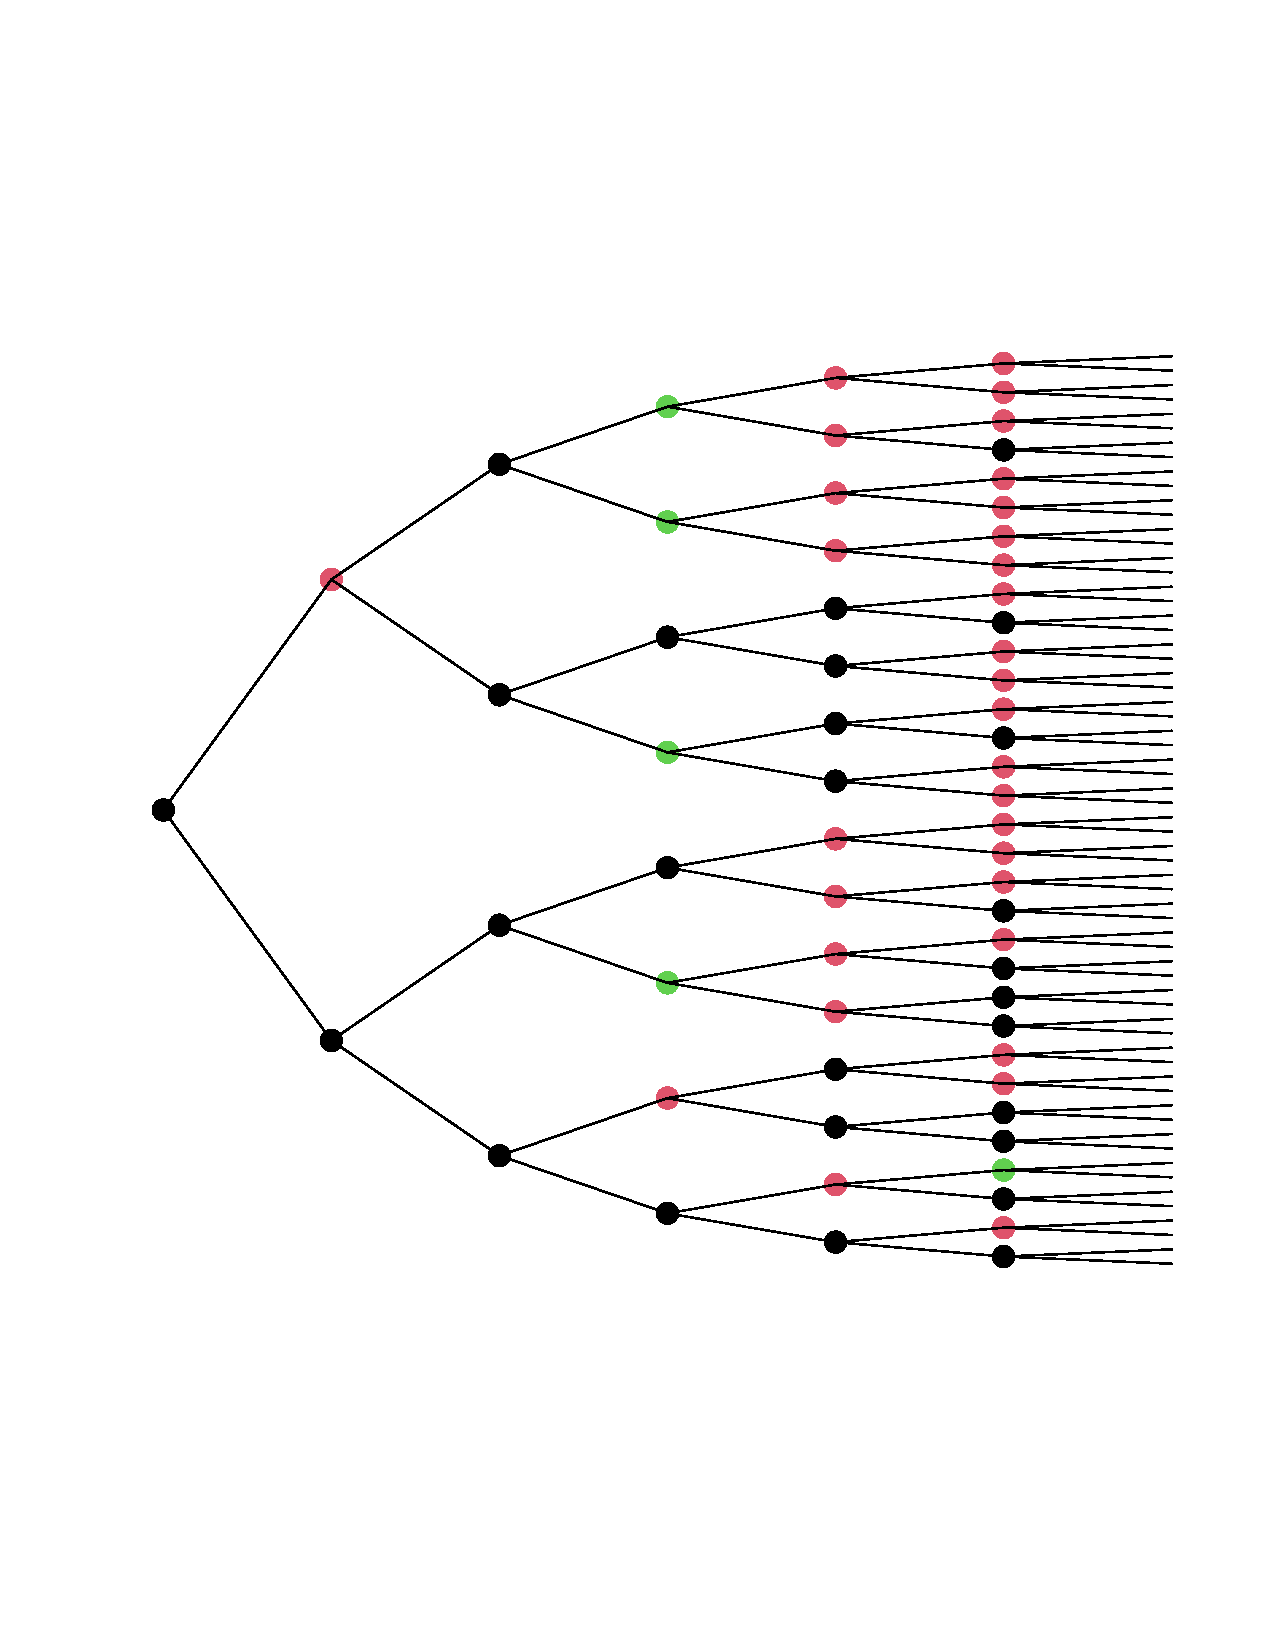
\includegraphics[width=0.45\linewidth]{figures/coronary_hc.pdf}}%
\hfill
\ffigbox{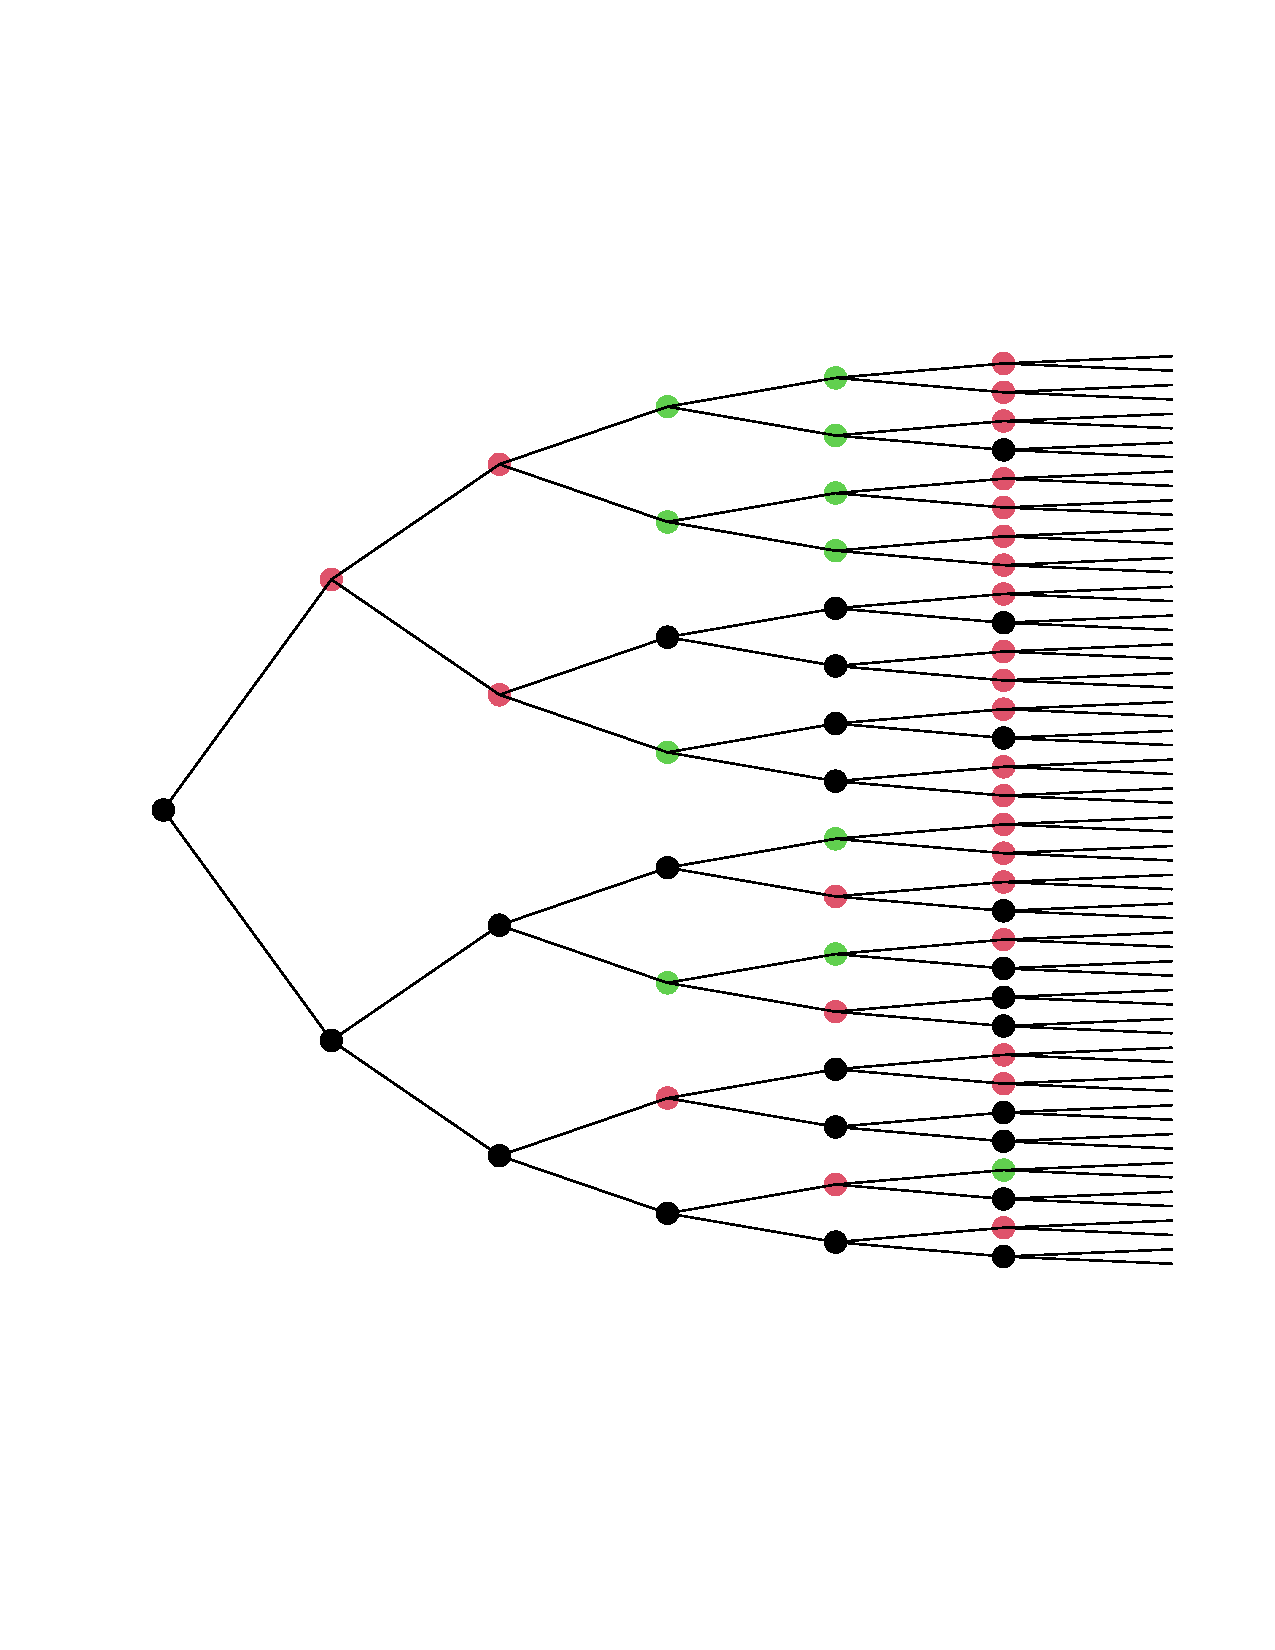
\includegraphics[width=0.45\linewidth]{figures/coronary_bhc.pdf}}
   \end{floatrow}

   
      \begin{floatrow}
   \centering
   \textbf{\hspace{5mm}Backwards joining \hspace{55mm} Hierarchical clustering}\par\medskip
\ffigbox{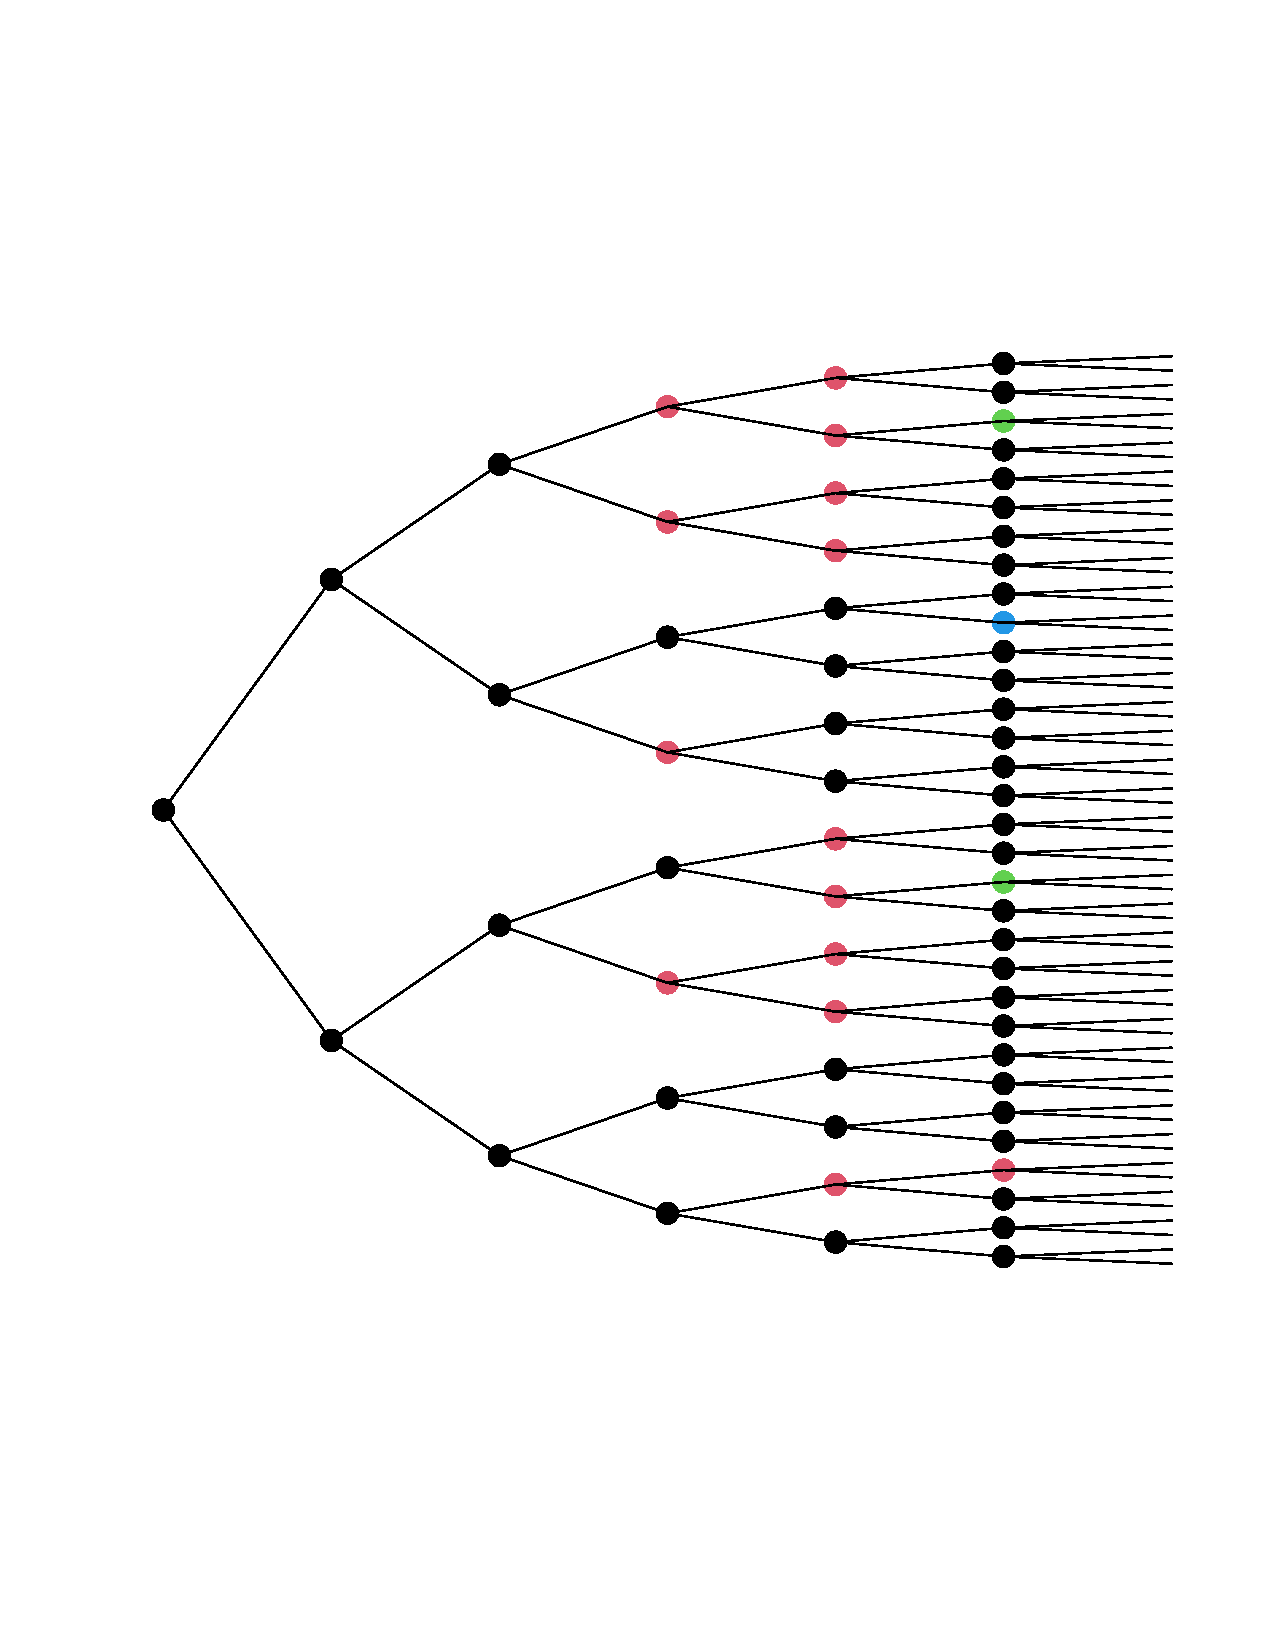
\includegraphics[width=0.45\linewidth]{figures/coronary_bj.pdf}}%
\hfill
\ffigbox{\includegraphics[width=0.45\linewidth]{figures/coronary_hclust.pdf}}%
   \end{floatrow}
   \caption{BIC-optimal staged trees learnt from the coronary dataset using the ordering 534126.}
\end{figure*}

\begin{figure*}
   \begin{floatrow}
   \centering
   \textbf{\hspace{10mm}Hill Climbing \hspace{50mm} Backwards hill climbing}\par\medskip
\ffigbox{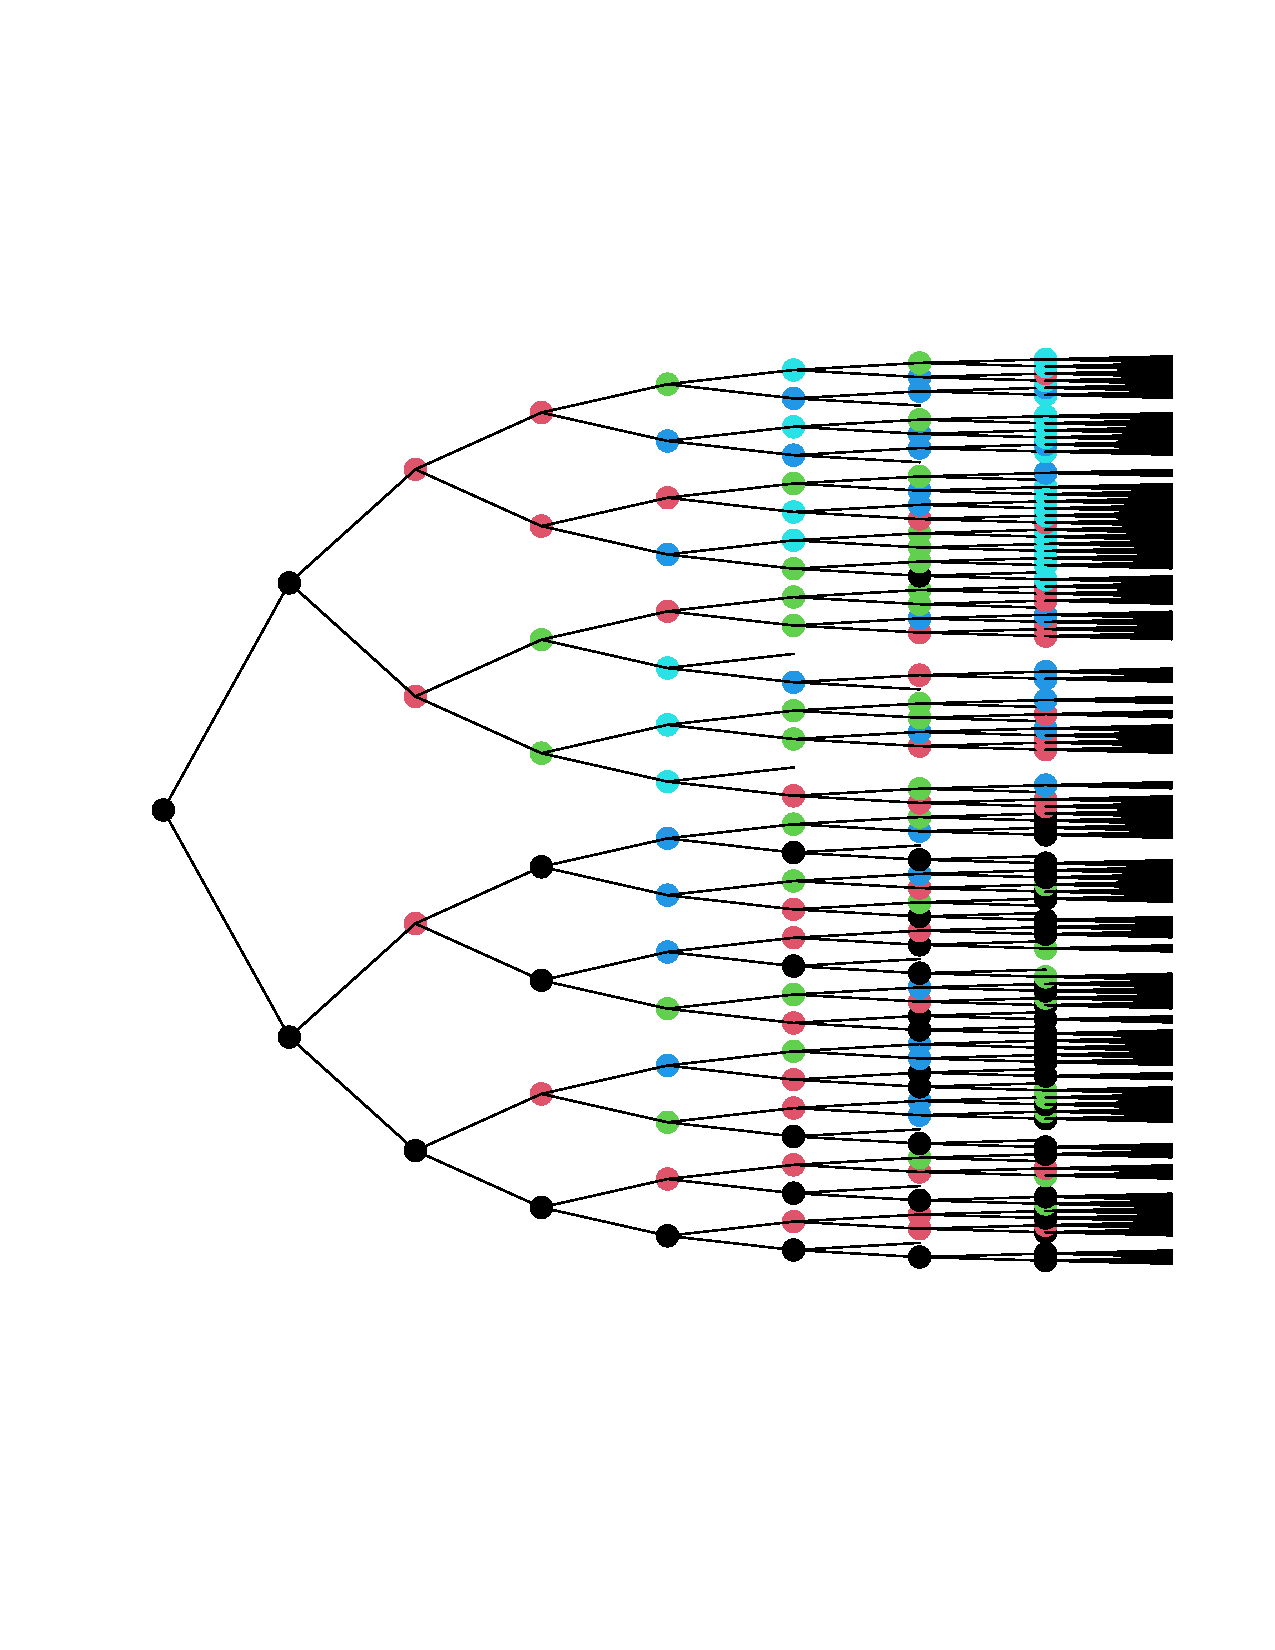
\includegraphics[width=0.45\linewidth]{figures/mice_hc.pdf}}%
\hfill
\ffigbox{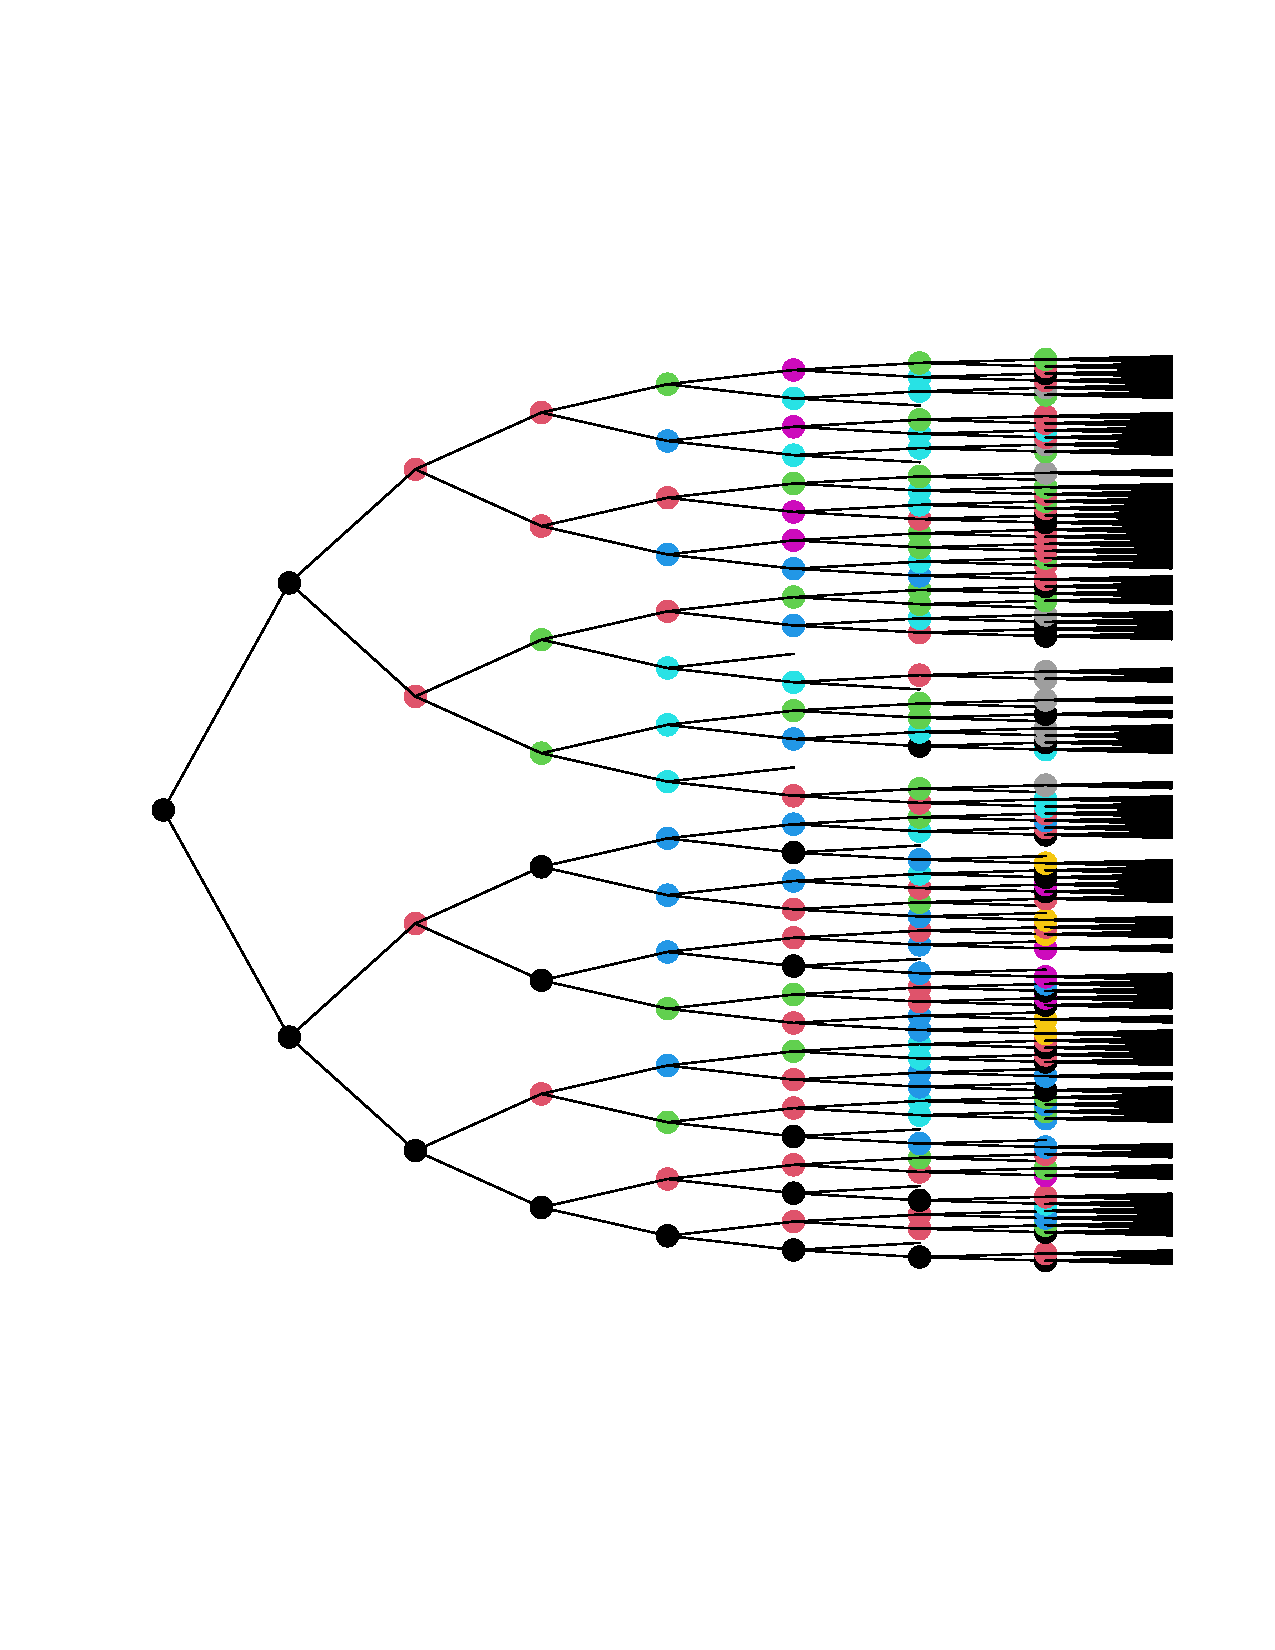
\includegraphics[width=0.45\linewidth]{figures/mice_bhc.pdf}}
   \end{floatrow}

   
      \begin{floatrow}
   \centering
   \textbf{\hspace{5mm}Backwards joining \hspace{55mm} Hierarchical clustering}\par\medskip
\ffigbox{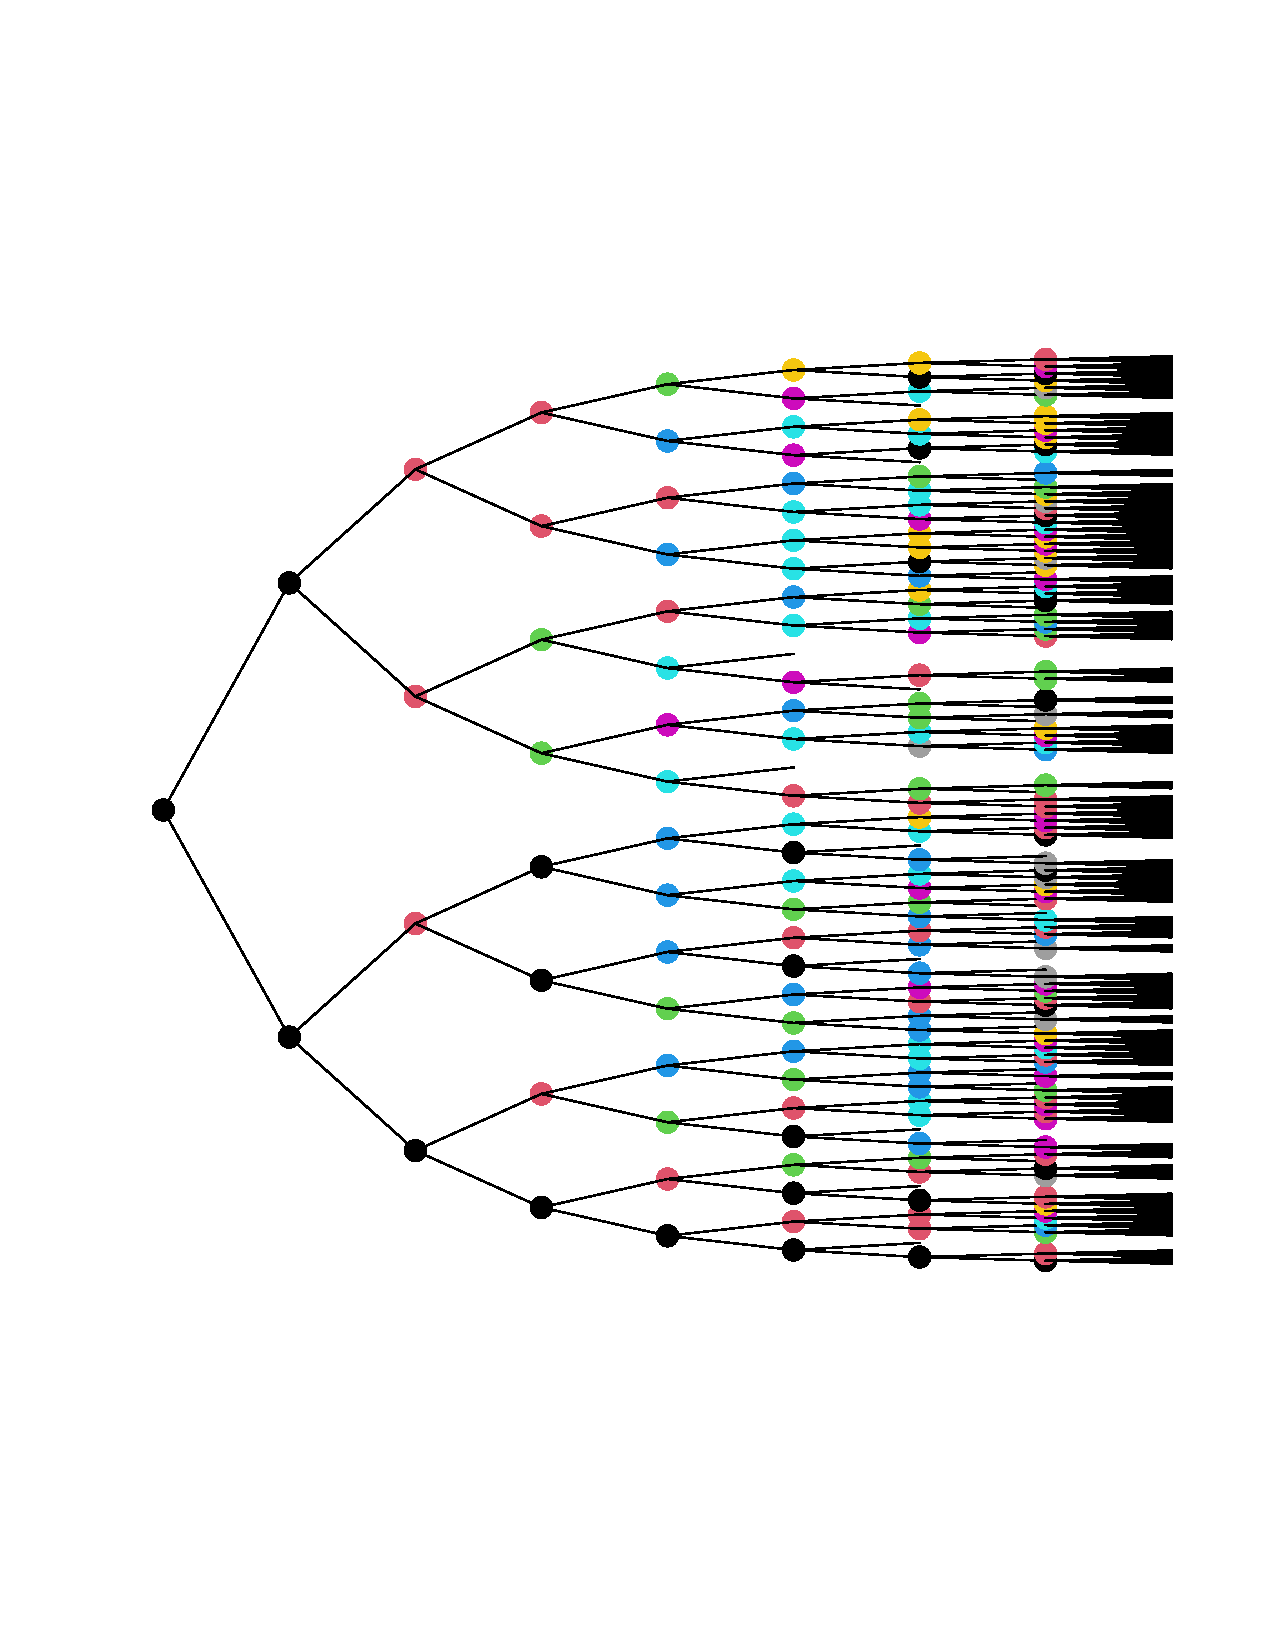
\includegraphics[width=0.45\linewidth]{figures/mice_bj.pdf}}%
\hfill
\ffigbox{\includegraphics[width=0.45\linewidth]{figures/mice_hclust.pdf}}%
   \end{floatrow}
   \caption{BIC-optimal staged trees learnt from the mice protein expression dataset using the ordering 32765148.}
\end{figure*}

\begin{figure*}
   \begin{floatrow}
   \centering
   \textbf{\hspace{10mm}Hill Climbing \hspace{50mm} Backwards hill climbing}\par\medskip
\ffigbox{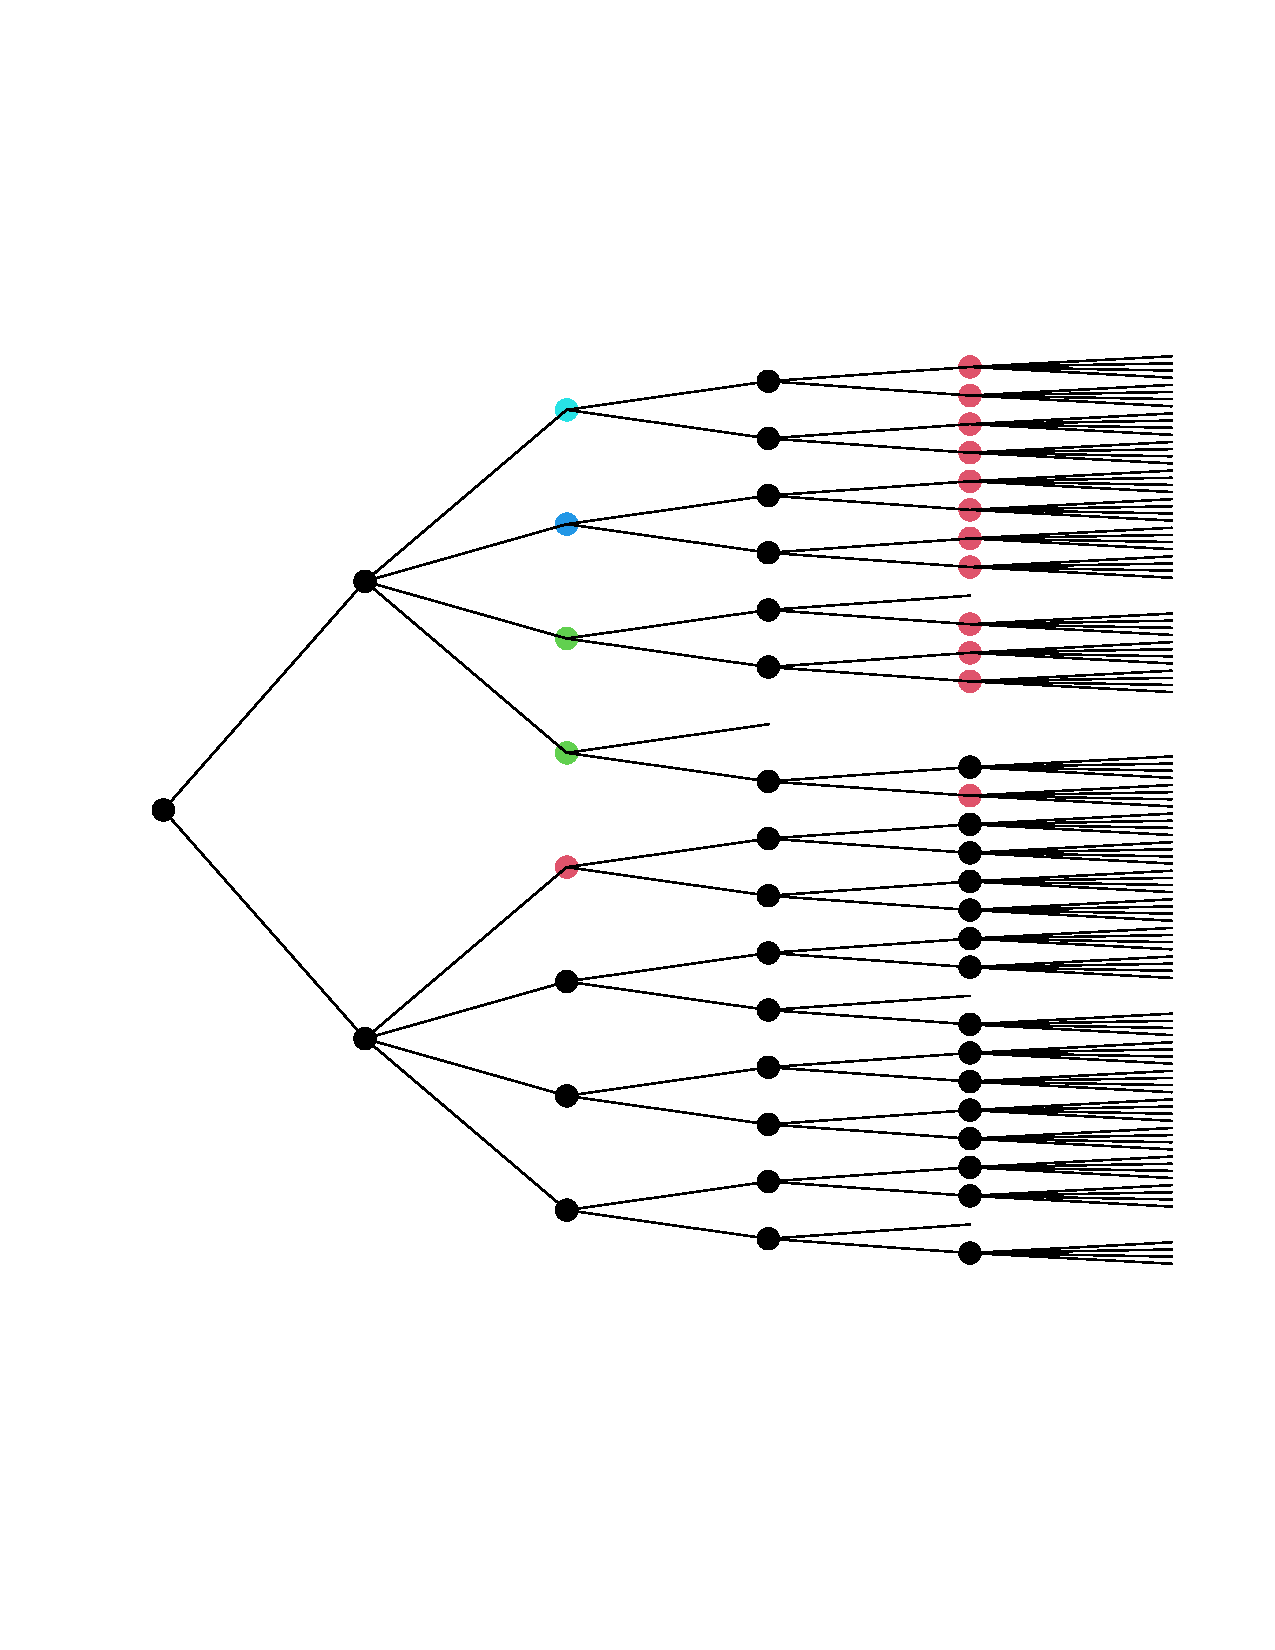
\includegraphics[width=0.45\linewidth]{figures/vitd_hc.pdf}}%
\hfill
\ffigbox{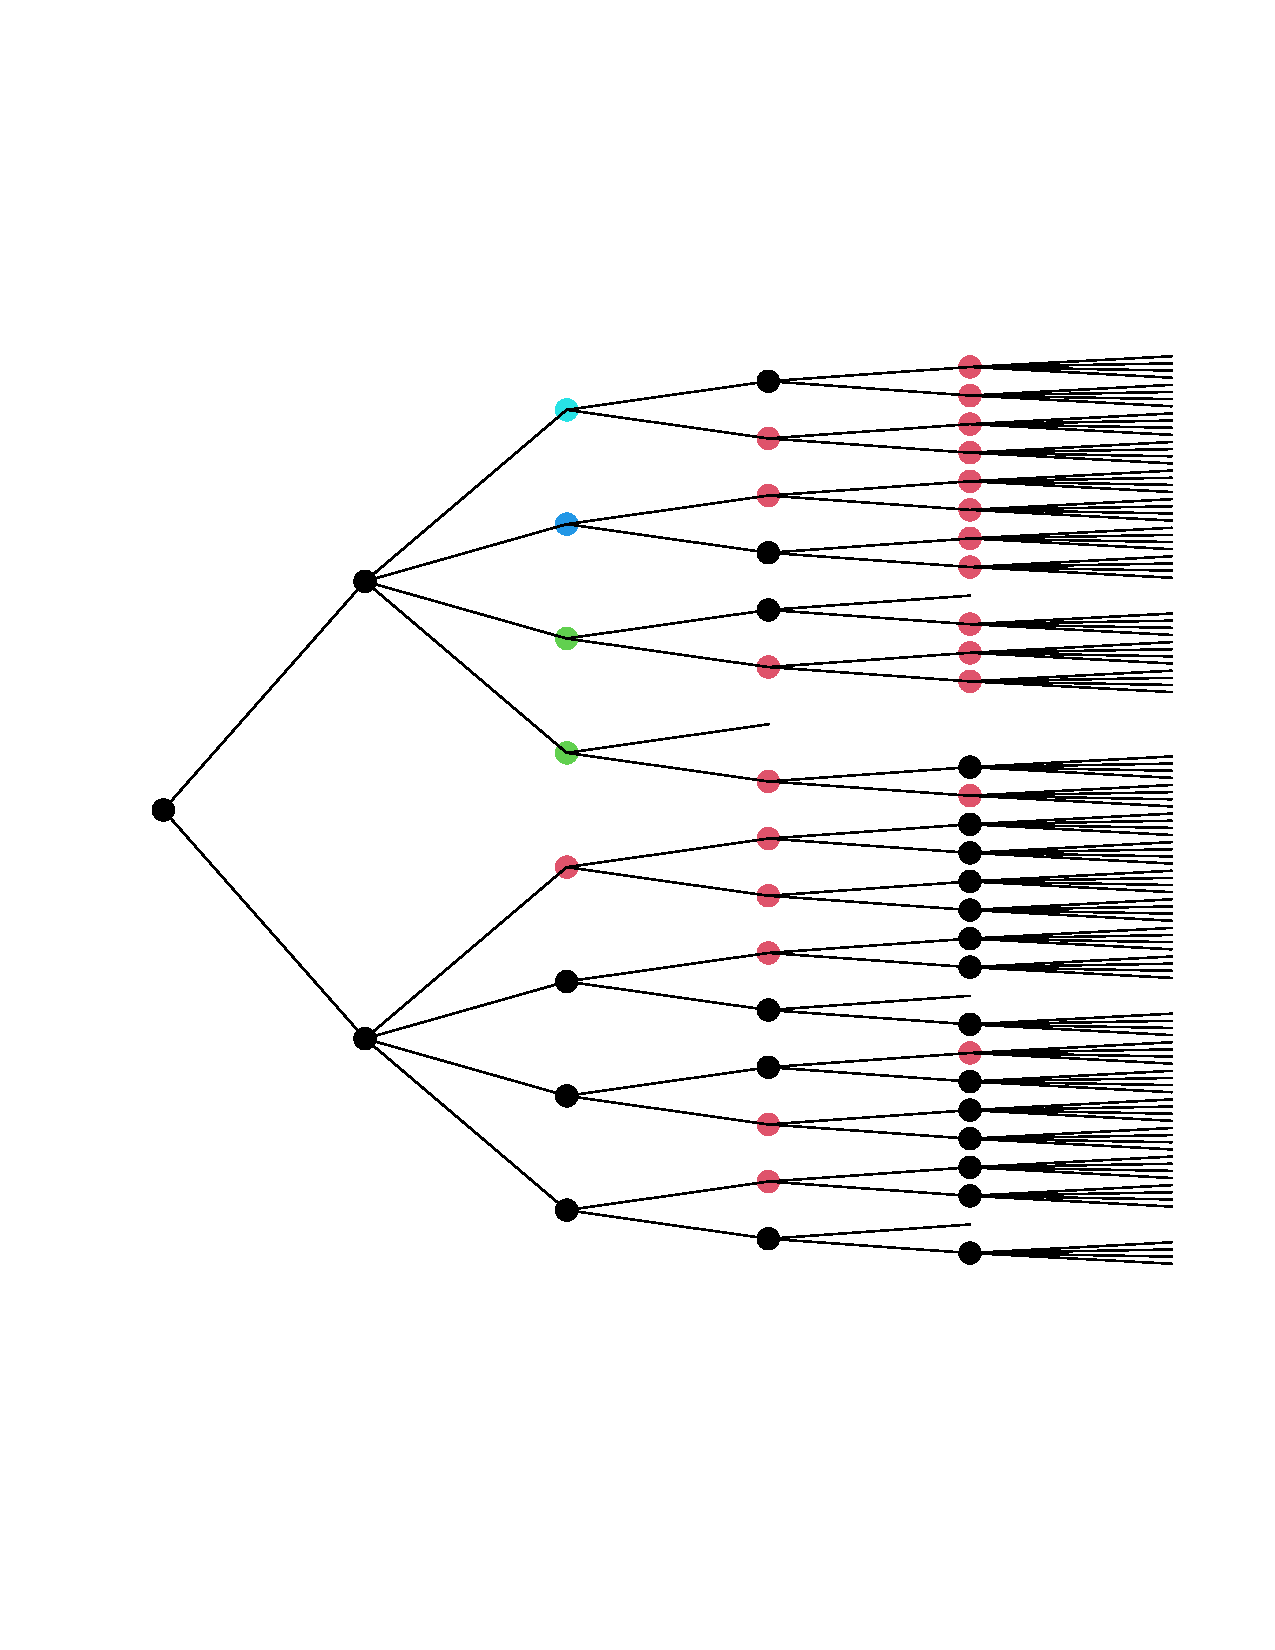
\includegraphics[width=0.45\linewidth]{figures/vitd_bhc.pdf}}
   \end{floatrow}

   
      \begin{floatrow}
   \centering
   \textbf{\hspace{5mm}Backwards joining \hspace{55mm} Hierarchical clustering}\par\medskip
\ffigbox{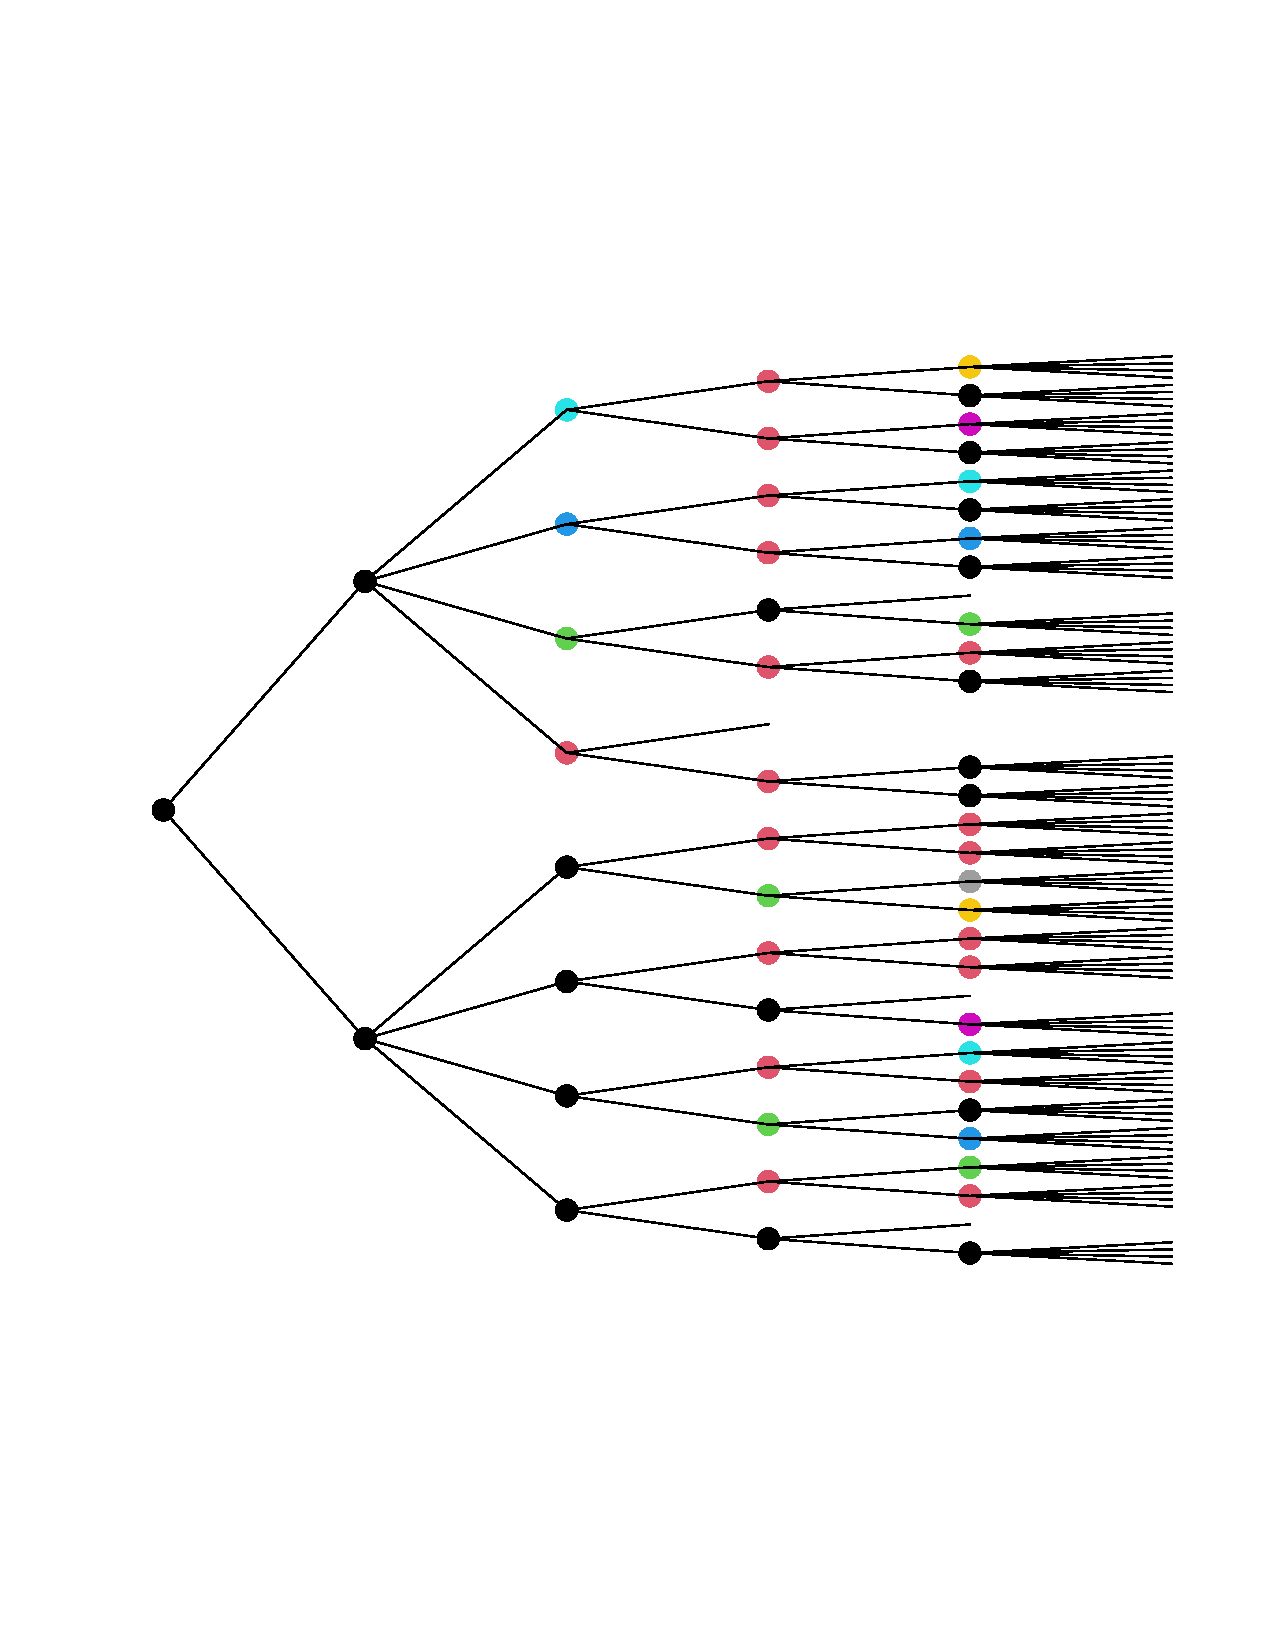
\includegraphics[width=0.45\linewidth]{figures/vitd_bj.pdf}}%
\hfill
\ffigbox{\includegraphics[width=0.45\linewidth]{figures/vitd_hclust.pdf}}%
   \end{floatrow}
   \caption{BIC-optimal staged trees learnt from the Vitamin D dataset using the ordering 53421.}
\end{figure*}

\begin{figure*}
   \begin{floatrow}
   \centering
   \textbf{\hspace{10mm}Hill Climbing \hspace{50mm} Backwards hill climbing}\par\medskip
\ffigbox{\includegraphics[width=0.45\linewidth]{figures/vitd_hc_gordering.pdf}}%
\hfill
\ffigbox{\includegraphics[width=0.45\linewidth]{figures/vitd_bhc_gordering.pdf}}
   \end{floatrow}

   
      \begin{floatrow}
   \centering
   \textbf{\hspace{5mm}Backwards joining \hspace{55mm} Hierarchical clustering}\par\medskip
\ffigbox{\includegraphics[width=0.45\linewidth]{figures/vitd_bj_gordering.pdf}}%
\hfill
\ffigbox{\includegraphics[width=0.45\linewidth]{figures/vitd_hclust_gordering.pdf}}%
   \end{floatrow}
   \caption{BIC-optimal staged trees learnt from the Vitamin D dataset using the ordering 32145.}
\end{figure*}
\end{document}